\documentclass[12pt]{report}
\usepackage{semtrans}
\usepackage{graphicx}
\usepackage{tabularx}
\usepackage[utf8]{inputenc}
\usepackage[Glenn]{fncychap}
\usepackage{ltablex}
\usepackage[T1]{fontenc}
\usepackage{enumitem}
\usepackage[margin=2cm]{geometry}
\usepackage{array}
\usepackage[table]{xcolor}
\usepackage{pdfpages}
\usepackage{appendix}
\usepackage[toc]{glossary}
\usepackage{titling}
\usepackage[cc]{titlepic}
\usepackage{hyperref}
\hypersetup{
    colorlinks=false,
    pdfborder={0 0 0},
}
\newcommand{\subtitle}[1]{%
  \posttitle{%
    \par\end{center}
    \begin{center}\large#1\end{center}
    \vskip0.5em}%
}

\makeatletter
\renewcommand*{\@makechapterhead}[1]{%
  \vspace*{10\p@}%
  {\parindent \z@ \raggedright \normalfont
    \ifnum \c@secnumdepth >\m@ne
      \if@mainmatter%%%%% Fix for frontmatter, mainmatter, and backmatter 040920
        \DOCH
      \fi
    \fi
    \interlinepenalty\@M
    \if@mainmatter%%%%% Fix for frontmatter, mainmatter, and backmatter 060424
      \DOTI{#1}%
    \else%
      \DOTIS{#1}%
    \fi
  }}
% For the case \chapter*:
\renewcommand*{\@makeschapterhead}[1]{%
  \vspace*{10\p@}%
  {\parindent \z@ \raggedright
    \normalfont
    \interlinepenalty\@M
    \DOTIS{#1}
    \vskip 40\p@
  }}
\makeatother

\makeglossary

\begin{document}
\setlength{\parindent}{0in}

\renewcommand{\thepage}{\roman{page}}

\title{XOXOmail}
\subtitle{Formal and secure messaging on a mobile platform}

\titlepic{
\begin{figure}[h!]
\begin{center}

\includegraphics[scale=0.1]{noshadow}
\end{center}
\end{figure}}

\author{Formal and secure messaging on a mobile platform\\ \\ \\ Kristin Tønnesen\\ Ida Katrine Thoresen\\ Nicklas Utgaard\\ Aleksander Sjåfjell\\ Lars Høysæter\\ Magnus Ulstein}
\maketitle
\clearpage



\chapter*{Abstract}

\textbf{This report} addresses the problem of communicating with the XOmail system from a mobile device. XOmail is a mail service that focuses on security and on getting the mail to its destination in a short time. During the project we created an Android application for cell phones and other devices that could provide the same security and stability as XOmail does on computers. The biggest issue of the project was how to make a handheld device secure enough to send important messages and to develop a user interface that is customized for small screens and easy to use. 
\newline
\newline
\textbf{The motivation} for working on this task is that even if there are a lot of different email applications for handheld devices today, none of them support the amount of security we need. The newest and most exciting part of the assignment was figuring out how to implement the required level of security. In addition, none of us have done extensive work with the Android framework before, so we are eager to learn more about the technology. Android applications are the new hot stuff in the development departments today, so getting the opportunity to learn about the newest products on the market is very interesting. 
\newline
\newline
\textbf{The demands} of our software project are, at first glance, quite simple. By implementing a mobile version of XOmail, the XOXOmail client, we will show what a working client might look like. It is important to note that we will focus on creating a proof-of-concept messaging client that uses the standards given by Thales. The primary focus is not on creating a fancy user interface, but rather on fulfilling the needs of the users. 
\newline
\newline
\textbf{The results} of this project will be unveiled as soon as the project has ended. It is, at this time, quite difficult to say anything about the results.



\chapter*{Preface}

This report was written for a project in the course TDT4290 Customer Driven Project at Norwegian University of Technology and Science (NTNU). The project was executed on behalf of Thales Norway AS between the 21th of August and the 22th of November.
\newline
\newline
The project team consisted of six students from the Department of Computer and Information Science at NTNU. Our task was to develop a mail application for handheld devices that could communicate with Thales' existing XOmail server.
\newline
\newline
The team would like thank our advisor Mohsen Anvaari for his advice and help throughout the project. We would also like to thank Reidar Conradi for his feedback. 
\newline
\newline
In addition we would like to thank our customer Thales and their contact persons Christian Tellefsen and Stig Bjørlykke. Their input and feedback have been invaluable and we would like to thank them for the cooperation. 
\newline
\newline
We would also like to thank the persons that set aside the time to participate in our usability tests and give us their valuable feedback about the design and usability of the XOXOmail application.


\tableofcontents

\listoffigures

\listoftables

\chapter*{Detailed contents}

\section*{Goal of the report}
This report documents the entire process behind developing the application. It describes what was done, why it was done and when it was done. The report contains summaries of all the pre-studies the group has been doing throughout the project, as well as the decisions made. It will describe the reason behind the actions and decisions. The report can also be used to monitor the development process of making the application the customer wants. In short, it describes how the prioritizations was made, and sums up what went well and what went not so well during the project.

\section*{What this report covers}
Chapter 2 - Project directive describes all the involved parties in this project. \\ 
Chapter 3 - Project planning gives an overview of how this task have been planned, how the team
\hspace*{5.5em}is organized and the quality assurance measures of the project. \\
Chapter 4 - Preliminary studies gives summaries of all the preliminary studies done in this project,
\hspace*{5.5em}as well as the decisions that have been made. \\
Chapter 5 - Requirements contains user stories and business requirements that detail how the
\hspace*{5.5em}application should look and behave. \\ 
Chapter 6 - Test plan explains how the code have been tested in this project. \\
Chapter 7 - Architectural description describes the architecture of the application, both backend
\hspace*{5.5em}and frontend. \\
Part II - Scrum process describes all of the sprints very carefully. It also includes the product
\hspace*{4.5em}backlog and the changelog. \\
Part III - Conclusion \& Reflection includes reflections on how the team has worked together, and
\hspace*{4.5em}describes disputes and agreements.

\section*{How this report is structured}
The report is divided into parts as well as chapters. This gives a much better overview of the report, and makes it a lot easier to find your way around it. It is divided into four parts; planning, preliminary studies, sprints and reflection.

\renewcommand{\thepage}{\arabic{page}}
\setcounter{page}{1}

\part{Planning \& Requirements}

%\chapter{Introduction}

	\chapter{Introduction}

This chapter is a technical introduction to the project. The purpose of this chapter is to give an overview of the task to be solved and the most important terms used in the report.

\subsection*{The existing product}
Thales has developed an information handling and transfer system called XOmail \cite{bib:xomail}, which has been in operational use for more than 20 years. In many ways, it could be compared to a regular, well-known email system. The first and biggest difference between regular email and and XOmail is that XOmail is developed with large formal organizations and military messaging procedures in mind. This is the reason why Thales has been delivering XOmail as a complete product to several European \gls{nato} member countries.  
\newline
\newline
The messages that are sent are defined to have a security label, which is a declaration of the required clearance level the receivers must have. The security label specifies that only people or groups with the required (or higher) security clearance can see the messages. Security is an important feature of XOmail, and it has never lost a message in 20 years of operation. 

\subsection*{What Thales wants us to make}
Thales’ existing product is a complete messaging platform for messaging in large organizations, but the current system is primarily made for use on typical computers with relatively large screens. What Thales wants to know is if it is possible to create a mobile messaging platform building on the existing infrastructure already in use by XOmail. It is important to note that this mobile platform will only have a subset of the functions that the original system has and the main focus is on security, efficiency and ease of use.
\newline
\newline
Since Thales has not tried to implement XOmail on mobile platforms, there is no existing framework to start with. Thales wants a prototype that demonstrates a possible solution to their problem. Security is of great importance, but the main focus should be on implementing functionality that is critical for showing the concept software.  
\newline
\newline
Even though XOmail primarily targets the military and other large organizations where security and security declarations are important, it is important to keep in mind that this software also should be well suited for other groups or organizations that have a need for a user-friendly portable system for sending urgent messages. A few of the possible candidates include paramedics, security firms and joint civilan-military operations or exercises.
\newline
\newline
For a summary of what Thales already has and what they want, see table \ref{tab:introcomparison} at page \pageref{tab:introcomparison}.

\subsection*{A short overview of the standards of XOmail}
XOmail is based on the \gls{nato} military messaging standard \gls{stanag}. This standard is used for both Strategic and Tactical messaging \cite{bib:stanag}. It has a number of special protocols used to support tactical messaging to support links with very low bandwidth.
\newline
\newline
The standard is based on binary encoded data, and there are limited libraries freely available for these protocols. Special attributes like information sensitivity and priority are defined by extensions to the Internet Mail RFCs. Our connection to Thales’ system goes through a XOmail \gls{smtp} gateway. \gls{smtp}, which is shorthand for Simple Mail Transfer Protocol \cite{bib:smtp}, is an Internet standard for electronic mail transmission over \gls{ip} networks. Messages to other users are sent by sending an email to the server with an address, and then the server handles the message headers and other important attributes. The messages are then pushed to the correct recipients via \gls{pami} \cite{bib:imap}, which is an abbreviation for Internet Message Access Protocol, and is one of the most prevalent Internet standard protocols for email retrieval. 

\begin{tabular}{l|l}
What Thales has&What Thales wants\\ \hline
An information handling and transfer system developed for large formal organizations and military messaging procedures&A system for handheld devices with a subset of the existing functions\\ \hline
A large number of ways of giving a message attributes&Focus on security label, priority and type\\ \hline
Extensive focus on security and reliability&Focus on security and usability\\ \hline
Support for a broad range of attachments&Support for images, text and video\\ \hline
\caption{Thales' current and wanted situation}
\label{tab:introcomparison}
\end{tabular}


%\chapter{Project directive}

	\chapter{Planning}

This chapter is about how we planned our project. The purpose of this chapter is to explain how our team is organized, who we are, why we do this project and how do it.

\section{Overall project plan}

\subsection{Project name}
XOXOmail

\subsection{Project sponsor}

The customer for this project is Thales Norway AS. Thales is a leading international electronics and systems group, focusing on defense, aerospace and security markets worldwide. The cutting edge technology in use at Thales offers capabilities unmatched in Europe for the development and deployment of mission-critical information systems proven in the field. The group’s civil and military business areas develop in parallel and share a common base of technologies to serve a single objective: the security of people, property and nations.
\newline
\newline
After Thales’ 50 years of industrial activity in Norway it is now one of Norway’s largest industrial centers of expertise for mission-critical IT and telecommunications solutions and one of the principal supplies of military communication systems to the Norwegian Armed Forces. [1]
\newline
\newline
See table \ref{tab:customer} at page \pageref{tab:customer}
\begin{table}
\begin{tabular}{l|l|l|l}
\textbf{Name} & \textbf{Office} & \textbf{Phone nr} & \textbf{E-mail} \\ \hline \hline
Sølve Conradi Olsen & Thales Norway & 907 80 179 & solve.olsen@thalesgroup.com \\ hline
Christian Tellefsen & Thales Norway & 959 98 765 & christian.tellefsen@thalesgroup.com \\ hline
Stig Bjørlykke & Thales Norway & 982 29 806 & stig.bjorlykke@thalesgroup.com
\end{tabular}
\caption{The customer representatives} \label{tab:customer}
\end{table}

\subsection{Involved Parties}

In this project there are only three involved parties: a) the customer b) the project team and c) the advisor. The customer, Thales, described in the section above was represented by Christian Tellefsen and Stig Bjørlykke. The project team consists of 6 students from the Department of Computer and Information Science (IDI) at the Norwegian University of Science and Technology (NTNU).The advisor was Mohsen Anvaari who was assigned to our team to guide and help us during the project period.
\newline
\newline
See table \ref{tab:projectgroup} at page \pageref{tab:projectgroup}
\begin{table}
\begin{tabularx}{\linewidth}{>{\setlength\hsize{.52\hsize}}X|>{\setlength\hsize{0.5\hsize}}X|>{\setlength\hsize{.3\hsize}}X|>{\setlength\hsize{.5\hsize}}X}
\textbf{Name} & \textbf{Address} & \textbf{Phone nr} & \textbf{E-mail} \\ \hline \hline
Ida Thoresen & Klæbuveien 143, 7031 & 936 68 688 & idakatt@stud.ntnu.no\\ \hline
Kristin Tønnesen & Lars Onsagersvei 12, 7030 & 986 28 958 & kristonn@stud.ntnu.no \\ \hline
Lars Høysæter & Innherredsveien 2a, 7014 & 900 31 814 & larssmor@stud.ntnu.no\\ \hline
Nicklas Utgaard & Odd Brochmanns veg 47, 7030 & 976 87 790 & nicklau@stud.ntnu.no\\ \hline
Magnus Ulstein & & 472 31 418 & magnuul@stud.ntnu.no\\ \hline
Aleksander Sjåfjell & Odd Brochmanns veg 60, 7030 & 456 01 212 & aleksasj@stud.ntnu.no
\end{tabularx}
\caption{The project group} \label{tab:projectgroup}
\end{table}

See table \ref{tab:advisor} at page \pageref{tab:advisor}
\begin{table}
\begin{tabular}{l|l|l|l}
\textbf{Name} & \textbf{Work} & \textbf{Phone nr} & \textbf{E-mail} \\ \hline \hline
Mohsen Anvaari & PhD-stud. NTNU & 405 70 403 & mohsena@idi.ntnu.no
\end{tabular}
\caption{Our advisor} \label{tab:advisor}
\end{table}

\subsection{Background for the project}

This project was given to us as an assignment in the course TDT4290 Customer Driven Project. Since the society is constantly changing, the technology must follow along with the enormous changes we see today. Because of these changes Thales found that they needed a handheld android version of their existing XOmail system. This new handheld system would help the users of XOmail so that they could also use it in the field and not only at the office. When able to use this mailing system not only in contact with a computer, the regular working day of Thales customers would be a lot easier, especially since their primary customer is the Norwegian military.

\subsection{Measurement of project effects}

Thales has proposed the following effects:
\begin{itemize}
\item{}Test user interface for message-based communication on a handheld device.
\item{}Make a prototype that can give inspiration for further product development and be used as a demonstration internally and to customers.
\end{itemize}

\newpage
\subsection{General terms}

\subsubsection{Technical Limitations}

\paragraph{Android}
Android is a quite new platform and none of us have been doing much programming in it before starting on this project. So learning how Android works and finding technical tools that Android supports is going to be a time consuming task. We will develop our project in Android version 2.2 with API level 8. The reason for choosing this version of Android is that we do not want to depend on features that only exist in the newer versions of Android. 

\paragraph{Screen}
The mail client will be used on devices with relatively small touch screens which means that the application must be carefully designed to accommodate the limited size. In addition we need to put a lot of thought into the design so that it becomes easy to use. The application must be designed to scale well with different screen resolutions.

\subsubsection{Non-technical Limitations}

\paragraph{Language}
The entire project is to be delivered in English, so we all have to write in our second language. This means that the report work will take more time than writing in Norwegian. 

\paragraph{Time}
We have a set timeframe of 13 weeks with a delivery deadline that cannot be changed. This gives us a set amount of time and we probably do not have the time to implement all parts of the application. We have to focus on the parts we find most important. The specified timeframe gives us challenges when it comes to planning and priorities of the different tasks.

\subsubsection{Tool Selection}

\paragraph{Git \& GitHub}
Git is an extremely fast, efficient and distributed version control system ideal for the collaborative development of software. It can be used to manage all your public and private repositories, and makes it easy to share and work with the same source code and documents [9]. GitHub is a hosting system that implements git and is free to use if you choose to share your source code with others. 

\paragraph{Google Docs}
Google Docs is a free web based service that offers users the ability to create and edit documents online. Google Docs lets us share documents easily and collaborate on the same document simultaneously.    

\paragraph{NetBeans IDE}
NetBeans IDE is an integrated development environment for developing with Java. It is written in Java and can run on Windows, Linux and OS X. NetBeans IDE is one of the most popular IDEs. Using a common IDE helps speed up the development process.

\paragraph{Apache Maven}
Maven is a build automation tool which is typically used with Java projects. It uses an XML file to describe the project, the project dependencies on other external modules and components, the build order, directories, and required plug-ins.   

\paragraph{JIRA with GreenHopper extension}
JIRA is an issue tracking system developed by Atlassian that is used for bug tracking, issue tracking and project management. When used along with the GreenHopper extension it adds support for agile development.

\paragraph{LaTeX}
LaTeX is a document markup language and document preparation system for the TeX typesetting program. LaTeX was chosen because of the high quality of typesetting which TeX provides.

\subsubsection{Organizational demands}
There are no organizational demands from Thales, but we agreed on a Scrum based approach. We decided that Scrum is a good lifecycle-model to use since it gives us a runnable product early that can be commented on during the project. This is a pilot project and the specifications are not fully completed, so many revisions are anticipated.

\subsubsection{Resources}
We are a very diverse group which can go both ways: in our favor and against it. We are all students working on a master's degree in computer science, but the programming experience of each member varies. Two of the group members have
programmed since they were about thirteen years old, while the rest started when they came to NTNU. All of us have at some point had a programming job, and are therefore used to working in teams.
\newline
\newline
Luckily, one might say, we all have different interests regarding what we would like to contribute with. While we agree that we all have to take our part of the programming, documentation and the report work, we can make use of our special intrests. As one of us likes to do documentation, another the report work and one of us has much experience in the setup of programming related tasks, we all have gotten our main roles accordingly.
\newline
\newline
Having a group consisting of people with different personalities gives us a challenging group dynamic. By having a daily stand up where everyone shares what they have done, what they will do and what they need to get it done, we are able to get a common understanding of what needs to be done and everyone can get in sync. 

\subsection{Duration}
The course staff has suggested a estimated 25 hour week for each student. This will give us a total of 1950 working hours since we are 6 students in our team and the project is distributed over 13 weeks.

\begin{itemize}
\item{}Project start: 21.08-2012
\item{}Project finish: 22.11-2012
\end{itemize}

\subsection{Schedule of results}

\subsection*{Milestones}
See table \ref{tab:milestones} at page \pageref{tab:milestones}
\begin{table}
\begin{tabular}{l|l}
Project start &  21.08.2012\\ \hline
Pre-delivery of project report & 14.10.2012\\ \hline
Final delivery of project report & 22.11.2012\\ \hline
Project presentation and demonstration & 22.11.2012
\end{tabular}
\caption{Milestones} \label{tab:milestones}
\end{table}

\subsection*{Sprints}
See table \ref{tab:sprints} at page \pageref{tab:sprints}
\begin{table}
\begin{tabular}{l|l}
Sprint 1 &  27.08.2012 - 16.09.2012\\ \hline
Sprint 2 & 17.09.2012 - 07.10.2012\\ \hline
Sprint 3 & 08.10.2012 - 28.10.2012\\ \hline
Sprint 4 & 29.10.2012 - 18.11.2012
\end{tabular}
\caption{Sprints} \label{tab:sprints}
\end{table}

\begin{figure}[htb]
\begin{center}
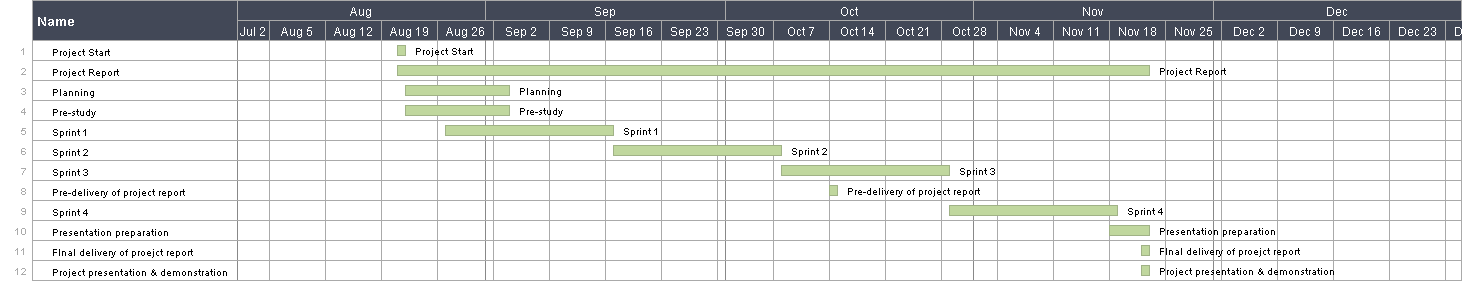
\includegraphics[width=\textwidth, height=2.5in]{foo}
\caption{Gantt-diagram for the entire project}
\end{center}
\end{figure}

%\chapter{Planning}

	\section{Project plan}

\subsection{Measurement of project effects}

Thales has proposed the following effects:
\begin{itemize}
\item{}Test user interface for message-based communication on a handheld device.
\item{}Make a prototype that can give inspiration for further product development and be used as a demonstration internally and to customers.
\end{itemize}

	\subsection{Limitations}

\subsubsection{Technical Limitations}

\paragraph{Android}\hfill
\newline
Android is a quite new platform and none of us have been doing much programming in it before starting on this project. So learning how Android works and finding technical tools that Android supports is going to be a time consuming task. We will develop our project in Android version 2.2 with API level 8. The reason for choosing this version of Android is that we do not want to depend on features that only exist in the newer versions of Android, and 2.2 is a version that is very common.

\paragraph{Screen}\hfill
\newline
The mail client will be used on devices with relatively small touch screens which means that the application must be carefully designed to accommodate the limited size. In addition we need to put a lot of thought into the design so that it becomes easy to use. The application must be designed to scale well with different screen resolutions.

\subsubsection{Non-technical Limitations}

\paragraph{Language}\hfill
\newline
The entire project is to be delivered in English, so we all have to write in our second language. This means that the report work will take more time than writing in Norwegian. 

\paragraph{Duration}\hfill
\newline
We have a set timeframe of 13 weeks with a delivery deadline that cannot be changed. This gives us a set amount of effort and we probably do not have the time to implement all parts of the application. We have to focus on the parts we find most important. The specified timeframe gives us challenges when it comes to planning and priorities of the different tasks.

	\subsection{Tool selection}
\subsubsection{Git \& GitHub}
\begin{wrapfigure}{r}{0.2\textwidth}
  \vspace{-40pt}
  \begin{center}
    
\includegraphics[width=60px,height=80px]{GitHub}
  \end{center}

\end{wrapfigure}
\gls{git} is an extremely fast, efficient and distributed version control system ideal for the collaborative development of software. It can be used to manage all your public and private repositories, and makes it easy to share and work with the same source code and documents \cite{bib:git}. \gls{github} is a hosting system that implements git and is free to use if you choose to share your source code with others. 

\pagebreak

\subsubsection{NetBeans IDE}
\begin{wrapfigure}{r}{0.2\textwidth}
  \vspace{-65pt}
  \begin{center}
    
\includegraphics[width=0.2\textwidth]{NetBeans}
  \end{center}

\end{wrapfigure}
NetBeans \gls{ide} is an integrated development environment for developing with Java. It is written in Java and can run on Windows, Linux and \gls{osx}. NetBeans \gls{ide} is one of the most popular \gls{ide}s. Using a common \gls{ide} helps speed up the development process.   

\subsubsection{Google Docs}
\begin{wrapfigure}{r}{0.2\textwidth}
  \vspace{-115pt}
  \begin{center}
    
\includegraphics[width=0.2\textwidth]{GoogleDocs}
  \end{center}

\end{wrapfigure}
Google Docs is a free web based service that offers users the ability to create and edit documents online. Google Docs lets us share documents easily and collaborate on the same document simultaneously.	

\subsubsection{Apache Maven}
\begin{wrapfigure}{r}{0.2\textwidth}
  \vspace{-35pt}
  \begin{center}
    
\includegraphics[width=0.2\textwidth, height=50px]{Maven}
  \end{center}

\end{wrapfigure}
\gls{maven} is a build automation tool which is typically used with Java projects. It uses an \gls{xml} file to describe the project, the project dependencies on other external modules and components, the build order, directories, and required plug-ins.   

\subsubsection{JIRA with GreenHopper extension}
\begin{wrapfigure}{r}{0.2\textwidth}
  \vspace{-40pt}
  \begin{center}
    
\includegraphics[width=80px,height=30px]{Jira}
  \end{center}

\end{wrapfigure}
JIRA is an issue tracking system developed by Atlassian that is used for bug tracking, issue tracking and project management. When used along with the GreenHopper extension it adds support for agile development.

\subsubsection{Wireshark}
\begin{wrapfigure}{r}{0.2\textwidth}
  \vspace{0pt}
  \begin{center}
  \vspace{-30pt}
    
\includegraphics[width=0.2\textwidth]{Wireshark}
  \end{center}

\end{wrapfigure}
Wireshark is a tool used for network troubleshooting and analysis. It captures network traffic and displays it to you through a graphical user interface. Wireshark is great for understanding how your application acts on a lower network layer.

\subsubsection{LaTeX}
\begin{wrapfigure}{r}{0.2\textwidth}
  \vspace{-35pt}
  \begin{center}
    
\includegraphics[width=0.2\textwidth, height=50px]{Latex}
  \end{center}

\end{wrapfigure}
LaTeX is a document markup language and document preparation system for the TeX typesetting program. LaTeX was chosen because of the high quality of typesetting that TeX provides.

\subsubsection{Fluid UI}

\begin{wrapfigure}{r}{0.2\textwidth}
  \vspace{-35pt}
  \begin{center}
    
\includegraphics[width=0.2\textwidth, height=50px]{fluidui}
  \end{center}

\end{wrapfigure}

Fluid UI \cite{bib:fui} is an online mobile app prototyping tool for Android and iOS apps. Fluid UI was chosen because it was a quick 
and easy way of creating interactive prototypes to share with the customer.

\subsection{Organizational demands}
There are no organizational demands from Thales, but we agreed on a Scrum based approach. We decided that Scrum is a good lifecycle-model to use since it gives us a runnable product early that can be commented on during the project. This is a pilot project and the specifications are not fully completed, so many revisions are anticipated.

\newpage

\subsection{Resources}
We are a very diverse group which can go both ways: in our favor and against. We are all students working on a master's degree in computer science, but the programming experience of each member varies. Two of the group members have
programmed since they were about thirteen years old, while the rest started when they came to NTNU. All of us have at some point had a programming job, and are therefore used to working in teams.
\newline
\newline
Luckily, one might say, we all have different interests regarding what we would like to contribute with. While we agree that we all have to take our part of the programming, documentation and the report work, we can make use of our special interests. As one of us likes to do documentation, another the report work and one of us has much experience in the setup of programming related tasks, we all have gotten our main roles accordingly.
\newline
\newline
Having a group consisting of people with different personalities gives us a challenging group dynamic. By having a daily stand up where everyone shares what they have done, what they will do and what they need to get it done, we are able to get a common understanding of what needs to be done and everyone can get in sync.

\subsection{Schedule of results}

\subsubsection*{Milestones}
See table \ref{tab:milestones} below for an overview of the milestones in our project.
\begin{table}[h!]
\begin{center}
\begin{tabular}{l|l} \hline
\textbf{Milestone} & \textbf{Date} \\ \hline \hline
Project start &  21.08.2012\\ 
Pre-delivery of project report & 14.10.2012\\ 
Final delivery of project report & 22.11.2012\\
Project presentation and demonstration & 22.11.2012\\ \hline
\end{tabular}
\end{center}
\caption{Milestones} \label{tab:milestones}
\end{table}

\subsubsection*{Sprints}
See table \ref{tab:sprints} below for an overview of the sprints that this project consists of.
\begin{table}[h!]
\begin{center}
\begin{tabular}{l|l} \hline
\textbf{Sprint} & \textbf{Duration} \\ \hline \hline
Sprint 1 &  27.08.2012 - 16.09.2012\\
Sprint 2 & 17.09.2012 - 07.10.2012\\
Sprint 3 & 08.10.2012 - 28.10.2012\\
Sprint 4 & 29.10.2012 - 18.11.2012\\ \hline
\end{tabular}
\end{center}
\caption{Sprints} \label{tab:sprints}
\end{table}

\begin{figure}[htb]
\begin{center}
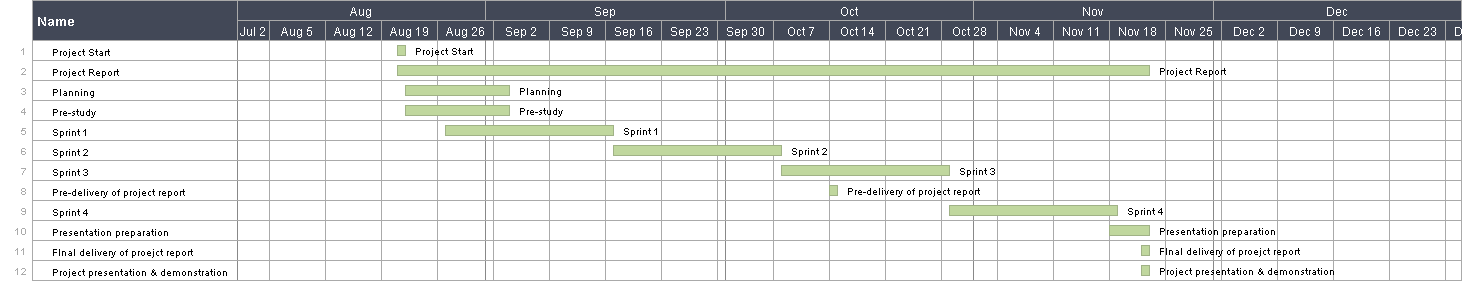
\includegraphics[width=\textwidth, height=2.5in]{foo}
\caption{Gantt-diagram for the entire project}
\end{center}
\end{figure}

	

\subsection{Concrete project work plan}

\subsection*{Sprints}
%See table \ref{tab:sprints} on page \pageref{tab:sprints}.
%\newline
%\newline
See table \ref{tab:allsprints} on page \pageref{tab:allsprints} for an overview of the planned effort for all the sprints in this project.
\begin{table}[h!]
\begin{center}
\begin{tabular}{l|l|l|l|l|l|l} \hline
\textbf{Phase} &  \textbf{Norm} & \textbf{S1} & \textbf{S2}  & \textbf{S3} & \textbf{S4} & \textbf{Total} \\ \hline \hline
Project management & 10 & 41h & 35h & 2h & - & 78h\\
Lectures & 10 & 4h & 8h & 15h & 9h & 36h\\
Planning & 7 & 26h & 99h & 93h & 48h & 266h\\
Pre study & 15 & 34h & 59h & 16h & - & 109h\\
Requirements specification & 20 & 18h & - & - & - & 18h\\
Design & 15 & 87h & 57h & 21h & 8h & 173h\\
Programming and documentation & 13 & 243h & 102h & 213h & 215h & 773h\\
Project evaluation & 5 & - & - & - & 20h & 20h\\
Presentation and demonstration & 5 & - & - & - & 60h & 60h\\ \hline
\end{tabular}
\end{center}
\caption{Plan for all the sprints} \label{tab:allsprints}
\end{table}




	\include{sprint-summary}

	

\section{Project organization}
We decided to use the scrum model for organizing our group. This means that we have a flat organizational structure where everyone contributes with what they are able to. Even in a flat structure, it is important to share responsibilities, so each person of the group got responsibility of a main focus area. If it becomes too much work for one person, we have decided that it is important that the work is delegated to the others.

\subsection{Organizational diagram}
See figure \ref{fig:organizationalchart} at page \pageref{fig:organizationalchart} for an organizational diagram that shows the internal structure of our group, as well as our connection to our advisor and Thales. Notice that even though we have a project leader, he is at the same level as all the others. This is to indicate that the project leader is not a big boss, but that we are all equally responsible for this project being a success.
\begin{figure}[hbt]
\begin{center}
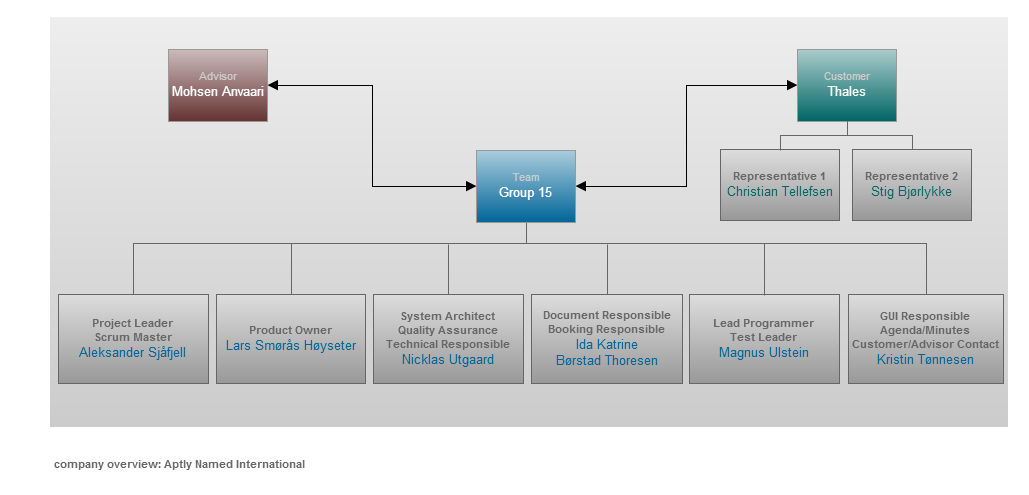
\includegraphics[width=\textwidth]{Organizational_Chart_v2}
\caption{Organizational chart} \label{fig:organizationalchart}
\end{center}
\end{figure}

\newpage

\subsection{Role allocation}
See table \ref{tab:roleallocation} at page \pageref{tab:roleallocation} for a role allocation table that shows what roles each person were assigned, as well as a short description of the role. The roles are merely a guideline for who is responsible for the depicted area. If the person should need more help, then we have all agreed to contribute to get the result we want. We are all in this together.
\begin{table}[hbt]
\begin{center}
\begin{tabularx}{\linewidth}{>{\setlength\hsize{.5\hsize}}X|>{\setlength\hsize{0.3\hsize}}X|>{\setlength\hsize{1\hsize}}X} \hline
\textbf{Role} & \textbf{Person} & \textbf{Responsibilities} \\ \hline \hline

Project leader & Aleksander & Make sure everybody does what they are supposed to and peacefully resolve disputes between participants \\  \hline
Scrum master & Aleksander & Make sure the team’s work conform to Scum standards and help the team do the best work possible \\ \hline

Booking of rooms & Ida & Booking rooms for the meetings and other activities \\ \hline
Document responsible & Ida &Keep track of what is to be contained in the project report, what has been written and what remains \\ \hline
Project report layout responsible & Ida &Find software to make tables and graphs, and check that all diagrams are similar in style \\ \hline

Responsible for graphical user interface & Kristin & Design the views and the interactions and setting up the MVC structure \\ \hline
Agendas, minutes of meetings & Kristin &Write agendas and minutes of meeting and send these out within the specified time limits \\ \hline
Customer/advisor contact & Kristin & Main contact person for customer and advisor \\ \hline

Product owner & Lars & Represent the stakeholders and ensure that the team delivers value to business\\ \hline

Test leader & Magnus & Lead the testing team \\ \hline
Lead programmer & Magnus & Responsible for having a general overview of the code. This means knowing what is to be implemented next, and seeing that this is done at the right time \\ \hline

System architect & Nicklas & Defining the system architecture \\ \hline
Technical responsible & Nicklas & Setup of Netbeans, Git and other tools that the team uses in the development \\ \hline
Quality assurance responsible & Nicklas & Make sure that all routines, templates and standards are followed \\ \hline

\end{tabularx}
\end{center}
\caption {Role allocation} \label{tab:roleallocation}
\end{table}

\newpage

\subsection{Weekly schedule}
See table \ref{tab:weeklyschedule} below for a weekly schedule that shows how we have allocated time for the Customer Driven Project. As we all have said how much we are able to contribute to the project, we have agreed to ensure that work outside of group work-hours must be done to reach the goal.
\begin{table}[h!]
\begin{center}
\begin{tabular}{l|l|l|l|l|l} \hline
 & \textbf{Monday} & \textbf{Tuesday} & \textbf{Wednesday} & \textbf{Thursday} & \textbf{Friday} \\ \hline \hline
\textbf{08-09} &  & Group work &  &  &  \\
\textbf{09-10} &  & Group work &  &  &  \\
\textbf{10-11} &  & Group work &  &  &  \\
\textbf{11-12} &  & Advisor meeting & &  &  \\
\textbf{12-13} & Group work & Group work & Customer meeting &  &  \\
\textbf{13-14} & Group work & Group work & Group work &  &  \\
\textbf{14-15} & Group work & Group work & Group work &  &  \\
\textbf{15-16} & Group work &  & Group work &  &  \\
\textbf{16-17} & Group work &  & Group work &  &  \\
\textbf{17-18} & Group work &  & Group work &  & \\ \hline
\end{tabular}
\end{center}
\caption {Weekly schedule} \label{tab:weeklyschedule}
\end{table}




	

\begin{table}


\begin{tabular}{ l|l|l|l|l } \hline
&	 &	 &\multicolumn{2}{c}{\underline{\textbf{Effort}}}	 \\
\textbf{Task}	 & \textbf{From date}	 & \textbf{To date}	 & \textbf{Est.} & \textbf{Act.}	 \\ \hline \hline
\textbf{Misc} & 21.08.2012 & 22.11.2012 & & \\ \hline
Project Management & 21.08.2012 & & 86 & 63.75 \\
Lectures & 03.09.2012 & & 47 & 31.5\\
Planning & 21.08.2012 & 26.08.2012 & 40 & 39 \\
Pre- Study &27.08.2012  & & 109 & 62.5\\ \hline
\bf{Sprint 1}	&\bf{27.08.2012} & \bf{16.09.2012} & \bf{271} & \textbf{186.5} \\ \hline
Planning & 27.08.2012 & 16.09.2012 & 26 & 95.5 \\
Design & 27.08.2012 & 16.09.2012 & 87 & 42.5\\
Implementation/Testing & 03.09.2012 & 16.09.2012 & 158 & 48.5\\ \hline
\bf{Sprint 2} & \bf{17.09.2012} & \bf{07.10.2012} & \bf{156} & \textbf{167} \\ \hline
Planning & 17.09.2012 & 07.10.2012 & 99 & 66.5\\
Design& 17.09.2012 & 07.10.2012 & 57 & 100.5\\
Implementation/Testing & - & - & - & -\\ \hline
\bf{Sprint 3}	 & \bf{08.10.2012} & \bf{28.10.2012} & \bf{241} & \textbf{250.5}\\ \hline
Planning & 08.10.2012 & 28.10.2012 & 93 & 58.5 \\
Design & 08.10.2012 & 28.10.2012 & 21 & 102\\
Implementation/Testing & 08.10.2012 & 28.10.2012 & 127 & 90\\ \hline
\bf{Sprint 4}	& \bf{29.10.2012} & \bf{18.11.2012} & \bf{}  &  \\ \hline
Planning & & &  &	 \\
Design& & & & \\
Implementation/Testing & & &  & \\ \hline
\textbf{Report \& Completion} & & & & \\ \hline
Report work & & & 273 & 364.25\\
Evaluation & & & & \\
Presentation && & & \\ \hline
\bf{Total} & & &\bf{}	& \\ \hline
\end{tabular}
\caption{Work breakdown structure} \label{table:wbs}
\end{table}


	\section{Quality assurance}
This section explains what we have planned to do to ensure quality in the project. Quality assurance is important to establish routines, not duplicate work or never lose any of the work. We want to ensure that all group members know how to do things, use the correct format and keep the deadlines.

\subsection{Time of response}
Agenda and questions for the meetings must be sent to the customer no later than 24 hours before the customer meeting is scheduled. 
Minutes of meeting should be sent to customer within 48 hours after the meeting, but preferably as soon as possible.
Approval of minutes of customer meeting should be done by the rest of the group before sending it to the customer. 
The customer should comment and approve of the minutes within 48 hours after receiving it from the group. 
Agenda and weekly documents should be sent to the advisor before Mondays at 14:00.
We should get approval and feedback of the documents sent to the advisor within 72 hours of having sent him the documents.
\newline
\newline
For a table of the agreed response times, see \ref{tab:responsetable} on page \pageref{tab:responsetable}.

\begin{table}[hbt]
\begin{center}
\begin{tabular}{l|l} \hline
\textbf{What} & \textbf{Time of response} \\ \hline \hline
Approval of minutes of customer meeting & 48 hours \\
Feedback on weekly documents & 72 hours \\
Approval of weekly documents & 72 hours \\
Answer to a question & 48 hours \\
Producing requested documents & 48 hours after approving request \\ \hline
\end{tabular}
\end{center}
\caption{Time of response table}\label{tab:responsetable}
\end{table}


\subsection{Routines for producing high quality internally}
To ensure high quality internally we will make sure every item produced is reviewed by a team member who did not work on the given item. We have planned to do this to increase the quality of the items and give the group members a better feel of the entire project and not just the parts they work on themselves.
\newline
\newline
Most of the working hours are planned together with other group members, either the entire team or in groups of two or three people. We want to ensure that there should always be someone to ask if any questions comes up, either in the 18 hours we have scheduled to meet physically each week or by communicating electronically. 

\newpage

\subsection{Routines for approval of phase documents}
Making sure that the different documents throughout the phases have the desired quality is a high priority for us. Therefore we have allocated one group member with the overall responsibility of putting together the different document parts and simultaneously reviewing of the documents. 
\newline
\newline 
We also want to make sure that the customer and advisor get opportunities to view the important documents that would affect the direction of our project. This way we will receive vital feedback and make the necessary changes according to the response of the advisor or customer. 
\newline
\newline
The visibility of the documents and progress is a part of the scrum method, meaning that the customer always has insight into what the group is doing and how far the group has progressed.

\subsection{Calling for a meeting with the customer}
In advance of all meetings with the customer we will send a call for the meeting, specifying time, place, intention, agenda, and background documents. It is important to specify preparations that have to be made by both the customer and the group prior to the meeting.
\newline
\newline
A calling for a meeting should be sent before Monday at 14:00 the week the meeting took place.


\subsection{Minutes of a customer meeting}
The group should write a summary of each meeting with the customer. The most vital points are decisions, actions (what, who and deadline) and clarifications that are important for further work on the project. The customer should approve the minutes of meeting to make sure there are no misunderstandings of decisions made. The minutes of meetings are part of the "contract" with the customer, not uncommon in normal settings.
\newline
\newline
The minutes of meeting should be sent to the customer as soon as possible and always before Friday the week the meeting took place. If the minutes are not approved by the customer, they should be rewritten and resent for approval.

\subsection{Calling for the weekly advisor meeting}
Calling for meetings should be sent before Monday at 14:00 the week the meeting was scheduled. The meeting with the advisor will normally takes place every Tuesday at 11:15 if no cancellation or exceptions are made.

\subsection{Agenda for the weekly meeting with the advisor}
We were given a template from the course administrative that was to be followed. This template can be found in appendix \ref{se:adag}.

\subsection{Minutes of the weekly meeting with the advisor}
Minutes from the last meeting will be attached to the next meeting call and is a fixed subject on the agenda.




	\subsection{Templates and standards}
The group has decided to make templates and standards for the most relevant document types. Even though it will take some time to create these in the beginning, we believe it will benefit us over time.

\subsubsection{Templates}

\paragraph{Phase documents}

\subparagraph{Sprint template}\hfill
\begin{enumerate}
\item{}Sprint Planning
\item{}Sprint Duration
\item{}Sprint Goal
\item{}Sprint Backlog
\item{}System Design
\item{}Customer Feedback
\item{}Conclusion
\end{enumerate}

\paragraph{Agenda for meetings}
We have made an template of an agenda that we use when we are planning an advisor meeting. The template make the work for our agenda responsible a lot easier.

\subparagraph{Agenda for advisor meetings}\hfill
\newline
\begin{enumerate}
\item{}Approval of agenda 
\item{}Approval of minutes of meeting from last advisor meeting
\item{}Comments to the minutes from last customer meeting or other meetings
\item{}Approval of the status report, which may be structured as follows:
\begin{enumerate}
\item{} Summary
\item{} Work done in this period
\begin{enumerate}
\item{}Status of the documents that are being created
\item{}Meetings
\item{}Other activities
\end{enumerate}
\item{}Problems – what is interfering with the progress or taking resources? Problems are often risks that have taken effect.
\item{}Planning of work for the next period
\begin{enumerate}
\item{}Meetings
\item{}Activities
\end{enumerate}
\item{}Other
\end{enumerate}
\item{}Review/approval of attached phase documents
\item{}Other issues
\end{enumerate}

\subparagraph{Agenda for customer meetings} \hfill
\newline
\begin{itemize}
\item{}Date
\item{}Project name
\item{}Calling by
\item{}Time and date 
\item{}Place 
\item{}Attendees 
\item{}Referent
\end{itemize}

\begin{enumerate}
\item{}Approval of agenda
\item{}Approval of minutes of meeting from last customer meeting
\item{}Case name
\item{}Other issues
\item{}Next meeting
\end{enumerate}

\subparagraph{Agenda for internal meetings} \hfill
\newline
\begin{itemize}
\item{}Date
\item{}Project name
\item{}Calling by
\item{}Time and date 
\item{}Place 
\item{}Attendees 
\item{}Referent
\end{itemize}

\begin{enumerate}
\item{}Approval of agenda
\item{}Approval of minutes of meeting from last internal, customer and advisor meeting
\item{}Case name * X
\item{}Other issues
\item{}Next meeting
\end{enumerate}

\paragraph{Weekly status reports for the advisor meetings}
\begin{itemize}
\item{}Date
\item{}Project name
\item{}Calling by
\item{}Time and date 
\item{}Place 
\item{}Attendees 
\item{}Referent
\end{itemize}

\begin{enumerate}
\item{}Activities done this week
\item{}Activities planned next week
\item{}Challenges ahead
\item{}Status summary
\item{}Milestones
\end{enumerate}

\paragraph{Minutes for meetings}

\subparagraph{Minutes for advisor meetings} \hfill
\newline
\begin{itemize}
\item{}Date
\item{}Project name
\item{}Calling by
\item{}Time and date 
\item{}Place 
\item{}Attendees 
\item{}Referent
\end{itemize}

\begin{enumerate}
\item{}Agenda approved
\item{}Minutes of meeting from last advisor meeting approved 
\item{}Comments to the minutes from last customer meeting
\item{}Approval of the status report
\item{}Summary
\begin{enumerate}
\item{}Work done in this period
\item{}Status of the documents that are being created
\end{enumerate}
\item{}Meetings
\item{}Other activities
\end{enumerate}

\subparagraph{Minutes for customer meetings} \hfill
\newline
\begin{itemize}
\item{}Date
\item{}Project name
\item{}Calling by
\item{}Time and date 
\item{}Place 
\item{}Attendees 
\item{}Referent
\end{itemize}

\begin{enumerate}
\item{}Topics of the meeting.
\item{}Decisions made.
\item{}Actions agreed upon.
\item{}Clarifications.
\item{}Time, date and place of next meeting
\end{enumerate}

\subparagraph{Minutes for internal meetings} \hfill
\begin{itemize}
\item{}Date
\item{}Project name
\item{}Calling by
\item{}Time and date 
\item{}Place 
\item{}Attendees 
\item{}Referent
\end{itemize}

\begin{enumerate}
\item{}Agenda approved
\item{}Minutes of meeting from last internal, customer and advisor meeting approved
\item{}Case name
\begin{enumerate}
\item{}Sub item
\item{}Sub item
\end{enumerate}
\item{}Other issues
\item{}Next meeting
\end{enumerate}

\subsubsection{Standards}

\paragraph{Organizing files}
paragraph{Google docs}\hfill
 We use Google Docs to organize our files so that our entire team can look at and change all the documents we have whenever they want. We have one folder that contains our entire project and in that folder we have subfolders to make the best overview possible. We try not to have too many files in each folder so that finding a specific document becomes as easy as possible.

\subparagraph{Git}\hfill 
We also use git so that it is easy to share all the code as well. When using git all the team members have access to change, read and use all the code files whenever they feel like it.

\subparagraph{Saving in gitHub}\hfill
All documents and Java files must compile before they are pushed to the repository.\newline
\textbf{Code repository structure}
\begin{verbatim}
kpro-app/
  res/ -- application specific resources -- resources used in the application
    drawable/ -- images for the application
    layout/ -- layouts for the the activies
    values/ -- common values for the application
  src/ -- java source folder
    main/java/no/ntnu/kpro/app -- the difference activites
  target/ -- build folder
kpro-instrumentation/
  src/ -- java source folder
    main/java/no/ntnu/kpro
	    app/ -- gui tests folder
		  core/service/ -- service tests folder
  target/ -- build folder
kpro-lib/
  res/ -- application specific resources
  src/ -- java source folder
    main/
      java/no/ntnu/kpro/core
        model/ -- application specific models
        service/ -- service related package
          factories/ -- factory classes
          implementations/  -- implementating classes
          interfaces/ -- all relevant interfaces
        utilities -- common javabased utilities
    test/
      java/no/ntnu/kpro/core/
        service/
          implementation/
  target/ -- build folder

\end{verbatim}
\textbf{LaTeX repository structure}
\begin{verbatim}
Backlog/		-- contains the teams backlog
Meetings/		-- agendas, feedback and minutes from every meeting
  Internal/
    Agendas/
    Feedback/
    Minutes/
  Mohsen Anvaari/
    Agendas/
    Feedback/
    Minutes/
  Thales/
    Agendas/
    Feedback/
    Minutes/
Project report/		-- the tentative complete report
Templates and standards/ -- templates in use
Weekly status reports/ -- weekly timesheets

\end{verbatim}


\paragraph{Naming of files}
All the files in our project have a name that starts with the date they were created so that they’ll be easier to find. The name also contains one or two words that explain what the documents consists.

sub\paragraph{Agendas}\hfill
\newline
"YYYY-MM-DD - Agenda - [Thales/Mohsen Anvaari/Internal]"

sub\paragraph{Minutes of meeting}\hfill
\newline
"YYYY-MM-DD - Minutes of Meeting - [Thales/Mohsen Anvaari/Internal]"

\paragraph{Coding style}
See \ref{tab:namingconventions} on page \pageref{tab:namingconventions} for code naming conventions.
\begin{table}
\begin{tabular}{l|l|l}
\textbf{Element} & \textbf{Convention} & \textbf{Example} \\ \hline \hline
Button & btn & btnSubject \\ \hline
ImageButtonr & imb & imbSubject \\ \hline
TextView & lbl & txtSubject \\ \hline
ImageView & imv & imvSubject \\ \hline
EditText & txt & txtSubject \\ \hline
Spinner & spr & sprSubject \\ \hline
ListView & lst & lstSubject \\ \hline
CheckBox & chb & chbSubject \\ \hline
RadioButton & rbt & rbtSubject \\ \hline
ToggleButton & tbt & tbtSubject \\ \hline
Layout & lay & laySubject 
\end{tabular}
\caption{Code naming conventions - all conventions need to have + identifer (lower camel-case) in addition to its unique three letter convention }\label{tab:namingconventions}
\end{table}


	

\section{Version control procedures}
Our group have created a systematic procedure for version control for all textual  and code documents. 

\subsection{Version control for code}
For source code management there are several viable options on the market, the big ones being Git and SVN. Although they do pretty much the same thing, there are some key differences in how they work which makes Git favorable over SVN. One key feature is performance, where Git greatly outperforms SVN. Git gives you the possibility of a hierarchy of repositories, which offers great flexibility. One upside being the local repository every user has on their computer. This enables the developer to work even though he does not have access to the remote repository. Lastly, and perhaps the most important difference comes with the branch/merge differences between the two tools. Git does this incredible well, while the general consensus is that SVN’s merge tool is tedious to use.  
\newline
\newline
In addition to technical differences between Git and SVN, it was the experiences of the developer team that finally made the decision to use Git for this project.

\subsection{Version control for code procedure}
All procedures assumes the use of a terminal similar to Bash, and that the current directory is the workspace of your IDE.
\newline
\newline
[]: optional arguments \& <>: argument

\subsubsection{Setup}
\begin{description}
\item[Description:] Setup of project (usually just once)
\item[Command:] git clone <git remote repository address>
\end{description}

\subsubsection{On programming session start}
\begin{description}
\item[Description:] Whenever a developer starts programming
\item[Command:] git pull [<remote repository> <branch>]
\end{description}

\subsubsection{On change}
\begin{description}[style=multiline]
\item[Description:] Whenever a developer changes some small functionality, feature or structure.
\item[Command:] git add <file> \#Repeat for all changed files \\ git commit -m “<commit message describing the changes made>” \\  \[git pull \&\& git push\] \#should only be done for if project builds
\end{description}

\subsubsection{On complete}
\begin{description}
\item[Description:]  Whenever a developer finishes with some functionality, feature,  structure or changes which influence 				any of the above.
\item[Command:]  git pull [<remote repository> <branch>] \\  \#Fix any merge conflicts \\ git push [<remote repository> <branch>]
\end{description}

\subsection{Version control for documents}
Version control for all documents is divided into two bulks. In the development stage of a document it resides within Google drive (Google docs), this gives us an rapid way of writing, editing and sharing all documents related to the project. Google drive also provides the necessary version control needed at this point. When a document or part of a document is finished it is then typesetted in latex and pushed to git. Once on git, the documents work in the same way as code would.  




	\subsection{Design guidelines}

\subsubsection{External resources}
\begin{itemize}
\item{}Create all strings in res/values/strings.xml for easy access and modifiability
\item{}Create all colors in res/values/colors.xml 
\item{}Use the same style for similar components throughout the application, and preferrably create styles in the res/values folder
\item{}Provide assets for all, e.g. images for low, medium and high screen densities
\item{}Consider using separate \gls{xml} files for portrait and landscape mode to optimize for both views
\item{}Font sizes: Use 12 \gls{sp} (scale independent pixels) for micro sized text, 14 \gls{sp} for small, 18 \gls{sp} for medium and 22 \gls{sp} for large. 
\item{}Be careful with the use of colors
\end{itemize}

\subsubsection{General from Android \cite{bib:android}}
\begin{itemize}
\item{}If it looks the same, it should act the same
\item{}Only interrupt the user if it is important
\item{}Keep texts brief 
\item{}Try to use pictures instead of long texts
\item{}Make important things fast
\item{}Be gentle if the user does something wrong and give clear recovery instructions
\end{itemize}

\subsubsection{Pure Android \cite{bib:pandroid}}
\begin{itemize}
\item{}Do not mimic \gls{ui} elements from other platforms
\item{}Do not carry over platform-specific icons
\item{}Do not use bottom tab bars
\item{}Do not hardcode links to other apps
\item{}Do not use labeled “Back” buttons on actions bars
\item{}Do not use right-pointing cares on line items 
\end{itemize}

	\subsection{Risk management}

\textbf{R1. Illness / Unavailability:} A member or members of the group become ill or unavailable. \\
\textbf{R2. Internal conflicts/disputes:} A conflict/dispute between 2 or more group members. \\
\textbf{R3. Problems with internal or external communication:} Misunderstandings between group members or with the customer. \\
\textbf{R4. Bad technical solution:}A bad technical solution/implementation is selected for the problem.. \\
\textbf{R5. Too much priority given to a certain task:} Too much time is spent working on a task. \\
\textbf{R6. Technical incompetence:} The group does not possess the technical experience to solve a task. \\
\textbf{R7. Inexperienced with software development method:} The group does not have the needed experience with the software development method. \\
\textbf{R8. Hardware failure:} A hardware failure halts the projects progress. \\
\textbf{R9. Chosen tools do not deliver:} Development tools cause the project to slow down. \\

Explanation of abbreviations used in table% \ref{tab:risks}:
\begin{itemize}
\item{}Probability:
\begin{itemize}
\item{}L = low
\item{}M = medium
\item{}H = high
\end{itemize}
\item{}Strategy and actions:
\begin{itemize}
\item{}Reduce = how to reduce the consequence
\item{}Accept = accept that the risk has occourred
\item{}Avoid = how to avoid that the risk happens
\item{}Transfer = how to transfer the consequence from a risk that has happened, so that the consequent gets minimized
\end{itemize}
\end{itemize}

%See tabel \ref{tab:risks} at page \pageref{tab:risks}
%\newline
%\newline
%\begin{longtable}

\begin{tabularx}
  \label{tab:risks}
\end{tabularx}
\begin{tabularx}{\linewidth}{>{\setlength\hsize{.3\hsize}}X>{\setlength\hsize{0.7\hsize}}X}\hline
Risk ID & R1 \\
Risk factor & Illness/Unavailability \\
Consequences & \textbf{M:} Absence may halt the project progress \\
Probability & M \\
Strategy \& actions & \textbf{Reduce:} Involve group members in different parts of the project to avoid complete halts for certain tasks \\
Deadline & Continuous \\
Responsible & Aleksander and Kristin \\ \hline
\end{tabularx}
\begin{tabularx}{\linewidth}{>{\setlength\hsize{.3\hsize}}X>{\setlength\hsize{0.7\hsize}}X}\hline
Risk ID & R2 \\
Risk factor & Internal conflicts/disputes \\
Consequences & \textbf{M:} Can result in problems with cooperation and thus causing the project progress to slow down \\
Probability & M \\
Strategy \& actions & \textbf{Accept:} The conflict can be a constructive discusion. \textbf{Reduce:} Stop the conflict by going between the parts and try to come to a common solution fast \\
Deadline & Continuous \\
Responsible & Aleksander and Magnus\\ \hline
\end{tabularx}
\begin{tabularx}{\linewidth}{>{\setlength\hsize{.3\hsize}}X>{\setlength\hsize{0.7\hsize}}X}\hline
Risk ID & R3 \\
Risk factor & Problems with internal or external communication \\
Consequences & \textbf{M:} Group members can end up doing things the wrong way or the group misunderstands the customer's wishes \\
Probability & M \\
Strategy \& actions & \textbf{Avoid:} Have frequent internal and external meetings to discuss what has been done and what needs to be done. \textbf{Accept:} If something is done the wrong way we have to do it again \\
Deadline & Continuous \\
Responsible & Everyone \\ \hline
\end{tabularx}
\begin{tabularx}{\linewidth}{>{\setlength\hsize{.3\hsize}}X>{\setlength\hsize{0.7\hsize}}X}\hline
Risk ID & R4 \hfill\\
Risk factor & Bad technical solution                                                \\
Consequences & \textbf{H:} The project will not be completed before deadline, or result in a poor quality \\
Probability & M \\
Strategy \& actions & \textbf{Avoid:} Plan well and conduct a thorough pre-study \\
Deadline & Sprint 1 \\
Responsible & Nicklas and Kristin \\ \hline
\end{tabularx}\\\\
\begin{tabularx}{\linewidth}{>{\setlength\hsize{.3\hsize}}X>{\setlength\hsize{0.7\hsize}}X}\hline
Risk ID & R5 \\
Risk factor & Too much priority given to a certain task \\
Consequences & \textbf{M:} May affect the quality of other important tasks \\
Probability & M \\
Strategy \& actions & \textbf{Avoid:} Plan the time distribution carefully \textbf{Reduce:} If we find that a task is given to much priority, let everybody on the team know about your concern, and then change the priority \\
Deadline & Continuous \\
Responsible & All \\ \hline
\end{tabularx}
\begin{tabularx}{\linewidth}{>{\setlength\hsize{.3\hsize}}X>{\setlength\hsize{0.7\hsize}}X}\hline
Risk ID & R6 \\
Risk factor & Technical encompetence \\
Consequences & \textbf{H:} The group will b unable to finish the project \\
Probability & H \\
Strategy \& actions & \textbf{Avoid:} Choose familiar solutions for the problems that occur and do a thorough investigation into unfamiliar technologies that are to be used \textbf{Transfer:} If one or more of the members get's a problem they can't solve, ask someone else \\
Deadline & Continuous \\
Responsible & Everyone \\ \hline
\end{tabularx}
\begin{tabularx}{\linewidth}{>{\setlength\hsize{.3\hsize}}X>{\setlength\hsize{0.7\hsize}}X}\hline
Risk ID & R7 \\
Risk factor & Inexperience with software development methods \\
Consequences & \textbf{M:} Lack of documentation and too much time spent on administration \\
Probability & M \\
Strategy \& actions & \textbf{Reduce:} Get familiar with the software development method early and be thorough with the documentation \\
Deadline & Continuous \\
Responsible & Everyone \\ \hline
\end{tabularx}
\begin{tabularx}{\linewidth}{>{\setlength\hsize{.3\hsize}}X>{\setlength\hsize{0.7\hsize}}X}\hline
Risk ID & R8 \\
Risk factor & Hardware failure \\
Consequences & \textbf{M:} may cause unexpected delays \\
Probability & M \\
Strategy \& actions & \textbf{Avoid:} Have version control and make information available from different locations \\
Deadline & Continuous \\
Responsible & Everyone \\ \hline
\end{tabularx}
\begin{tabularx}{\linewidth}{>{\setlength\hsize{.3\hsize}}X>{\setlength\hsize{0.7\hsize}}X}\hline
Risk ID & R9 \\
Risk factor & Chosen tools do not deliver \\
Consequences & \textbf{M:} may halt the project progress \\
Probability & M \\
Strategy \& actions & \textbf{Reduce:} Find out what the most suited tools on the market is and choose one that is better suited. \\
Deadline & Preliminary study \\
Responsible & Nicklas  and Ida\\
\hline
\caption{Table for handling of risks}
\end{tabularx}
%\begin{tabular}{ll}
%	\hfill&\hfill\\
%	
%\end{tabular}
%\end{longtable}
%\end{document}






%\chapter{Preliminary study}

	\chapter{Project study}

This Chapter will cover the preliminary studies carried out in this project and will provide an understanding of what the problem to be solved, what solutions exist already and what solutions we have chosen.

\section{Problem description}

\subsection{Thales}
Thales wants us to develop a message service that is custom made for mobile users, with a user-interface that has good affordance and is easy and effective to use.
\newline
\newline
The users of this application are people who need a reliable and secure way of communicating with more or less time dependent information. Users are also expected to only have access to either tablets or mobile phones, not computers.

\subsection{Functionality}
The application's functionality should be similar to a normal email client, but with a user-interface that is custom-made for smaller screens, short messages, military domain specific  attributes, reliability adjustments for field use and security adjustments for handling classified information. The application should use the Simple Mail Transfer Protocol to communicate with Thales' XOmail \gls{smtp} gateway.
\newline
\newline
The application should not use bandwidth when it is not sending or receiving messages. The application should also be able to receive an updated address book from the server.

\subsection{The solution}
As per the customer requirements, the solution is to be implemented on Android based smartphones or tablets (Requirement 1.1 and 1.2) and the user-interface should be fitted to the screen size of the given device (2.1). It should support bandwidths as small as 64 kbps (2.2) and communicate with a XOmail server through \gls{pami}/\gls{pop} and \gls{smtp}(1.4 and 2.3). The application should also work with normal mail servers, but with reduced functionality (2.4).
\newline
\newline
The messages sent with our solution should be able to support text, pictures and video attachments (3.1). The media should be accessed from the local storage on the phone or from other applications (3.2). A user should be able to create, edit, send, answer, forward and delete messages as well as browse and open received and sent messages (3.3)

\subsection{Military attributes}
The messages that a user sends should support certain military attributes, these include precedence, type and security label. Precedence is an indicator that indicates the level of urgancy, and type indicates the type of the message. Security label on the other hand says something about the reciever of the massage, and not the massage itself. The security label says what security clearance the receiver must have to be able to open the message.
\newline
\newline
One should also be able to ask for a delivery report and a receipt notification from the recipient of the message sent. The one who sends the message should be able to see the status on the delivery report and receipt notification.

\subsection{Instant messages}
Another message functionality is the ability to send instant messages with predefined military attributes to a predefined reciever. The reciever can be a group or a single reciever. These can include predefined text or information from another application. It should also be possible to send messages with content that is created by other applications on the device.
\newline
\newline
When a message that is sent from the application fails, the user should get a notification and the message should be sent again automatically. These messages should also be sorted by priority.

\subsection{High priority messages}
If a high priority message arrives on a given user’s phone, the application should alert the user in a convenient way and make it easy to access the newly arrived message. The application should stop the sending of all other messages when a user sends a message with high priority, and instead give the resources to the high priority message.  

\subsection{Security}
Security is also an important issue in the application. Communication with the server should be encrypted with \gls{ssl1}, messages should be signed with \gls{emims} when being sent, \gls{emims} signed messages should be verified on receive and private keys for
signing mail should not be stored in cleartext.


	\section{Current system}\label{sec:currsys}

At the moment, there are no mobile solutions to the already existing XOmail system on computers.

\subsection{XOmail - Secure message based information handling}

XOmail is a message system tailored for messaging within military organizations. The messaging functions within the system are suited for the needs of large organizations with the ability to differentiate between social messages to the entire organization and personal messages to individual users. XOmail has the ability to send messages to predefined  distribution lists where the messages gets distributed based on a given criteria like the subject of the message. 
\cite{bib:XOhome}
\newline
\newline
The system also has several APIs that can be accessed by other applications. XOmail supports message coordination for use in the drafting process, as well as the ability to have a release authority for a drafted message. Another feature of XOmail is the ability to add precedence to messages, giving high priority messages access to resources and communication channels before messages with lower precedence. This is very important in a military setting. 
\cite{bib:XOhome}
\newline
\newline
XOmail has also a high focus on security, and offers security for the messaging platform, servers and gateways. The system also has an extensive administration tool that can be accessed both locally and remotely.
\cite{bib:XOhome}
\newline
\newline

\begin{figure}[h!]
\begin{center}
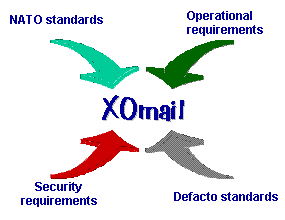
\includegraphics{xomaillogo}
\end{center}
\caption{XOmail logo} \label{fig:xomail}
\end{figure}

	\section{Planned solution}

The base evaluation of the project is: can it securely and reliably send and receive XOmail messages to Thales’ military servers from an android phone. Naturally, that is easier to state than to qualify. 
\newline
\newline
Sending and receiving is easy to test. Security is more complex. When can an application be called “secure”? When is a system “reliable”? Our best bet there is to document all our choices and their implications, as well as things that our customer could do with their additional resources if they were to extend our simple prototype. 
\newline
\newline
As such, we have listed Sending and Receiving as functional project requirements, as well as a number of other basic requirements of a messaging system. Most of these were given to us directly by the customer, with a relatively short period of discussion and clarification. 
\newline
\newline
The non-functional requirements are mostly related to usability, security, and performance. These are all difficult to quantify, and extensive documentation has gone into doing so, as will be seen throughout this document. 

	\section{Similar solutions}
As there is few, If any solutions that give the same capabilities as what is expected of this application, there will be given an overview of existing applications that do fullfill some of the requirements of XOXOmail. 
\newline
\newline
A very important aspect of XOXOmail is the signing and verification part. This is an app that will be used by important persons with security grading, and a message from such a person should be verified. 

\subsection{Signing and verification}
In order for this to be an informative in depth analasys, it is appropriate with a general overview first, which first gives an introduction to public key encryption, then a short overview of S/MIME, and then use of SMIME in XOXOmail.

\subsubsection{Public key encryption}
Public key encryption is used when you want to secure data in such a way that only the reciever can open the message. It involves using two separate keys; one secret key and one public key. [10]
\newline
\newline
If I want to send a message to, lets say John, I first have to get Johns public key. His public key is available to everyone who wants it. It is not a problem if a unwanted person gets it. This is the reason it is called public key. When he has given me his public key, I can then use it to encrypt the message. One might ask: What is the reason for using a public key? Does that give any security? The answer is yes. There is a mathematical relation between the private and public key. If you know the public key, it is nearly impossible or very expensive to calculate the private key. Therefore, by using John public key to encrypt the message, I know that he is the only one that can open it. It is only the private key of John that will open the message. 
\newline
\newline
Another concern could be: How does John know that I was the sender of the message? By just using the private-public key scheme as explained above, this is not possible. But by introducing digital signing, this is possible.

\subsubsection{Digital signing}
Signing is just what it sounds like. It is a way of signing data so that the receiver of the document  knows that the sender is who he say he is [11]. In our example, this means that John wants a way of knowing that I am the sender. This is done by digital signing, which first consists of computing a message digest, which is just a hash of the message. This hash is then used to encrypt the hash. Then, when John receives the message he will use my public key to decrypt the signature, and thereby receiving the hash. If John then creates a hash of the received document, and if it matches the hash of the signature, he knows that the message is from me and that it is not tampered. So far, so good. 

\subsubsection{Verification}
But what if a third person wants to deceive me, and sends a message to John with my public key? For John knows that the message was sent by someone with my name, but are we sure that it is I that sent it? The solution to this is a Certificate Authority, also known as CA. The CA creates a digital certificate for my public key, which ensures that it really is from me. If John only approves messages that has a valid certificate, he knows that the message really does come from me.

\subsubsection{S/MIME}
S/MIME is an abbreavations for Secure/Multipurpose Internet Mail Extensions. It is a standard for public key encryption and signing of MIME data [12]. MIME content is text in character sets that differ from ASCII, non-text attachments, message bodies with multiple parts and non ACII headers. It is just an extension of the well known mail format so that it is possible to send content other than plain text.

\subsubsection{Available apps with signing functionality}
An already existing app for sendining signed messages i X509 tools.

\subsubsection{X509Tools}
This is an application that has the ability to send mail with S/MIME capabilities, but its main purpose is not for sending mails. The main purpose is to give these capabilites to external mail clients via an interface. It also has an Certificate Store which can be used to check certificates already present on the phone. 

\subsection{Sending mail}
There are many applications available for sending mail from an Android phone. This section will first give a superficial overview of other programs, and then a short summary of what these provide, that may be useful to us.

\subsubsection{Built in client}
The first and most obvious clients for sending mail is the built in Android mail client which is what one can say is abandonware. It is often outdated and lacks a lot of basic functions.

\subsubsection{GMai}l
One of the most used email clients for phones is the GMail app. It is developed by Google, and is therefore seen as secure app with a streamlined design. Unfortunately, it stops there. Google has been neglecting all problems that it has, and new features are not coming. Functions like sorting of mail is lacking and it is not very reliable. It often shows messages received for hours before the message actually is in the inbox. Fortunately, there exists a fork of GMail, called K-9

\subsubsection{K-9 Mail}
K-9 Mail has all the features that one would say is missing in GMail, and then some. Most features are configurable. It is possible to edit app polling settings, show a short exercept of the message text. The message selection checkboxes can be temporarily hidden. So can the starring of the messages. It is even possible to adjust font sizes and date formats. The clue here is configurability.

\subsubsection{MailDrod}
It has many of the same functions as in K-9 mail, but also incorporates spell checking, changing font sizes and colors on email messages

	\newpage

\section{Software development model}

This section will describe the two different options we had for a software development model; waterfall and agile.

\subsection{Waterfall}
The waterfall model is a sequential design process that is often used in software development processes, in which progress is seen as a flow of water through the phases of conception, initiation analysis, construction, testing, production/implementation and at last maintenance \cite{bib:waterfall}. 
\newline
\newline
This is a model that was originally used in hardware industry, but in lack of a better model, was adapted for software development. In the waterfall model, each of the stages is sequential, and another phase starts where the previous ends. There is no room for different approaches here. Before implementations of a software product, the documentation has to be carved in stone. If, for example, the documentation is only half done, it will ruin the whole process. Therefore, one has to be entirely sure that a phase is over before a new one begins. 

\subsection{Agile}
Agile development is based on interative and incremental development, and promotes a workflow process that embraces change \cite{bib:agile}. The Agile Manifesto states that we get better software by concentrating on the software itself, the customers receiving the software and focusing on the team dynamic of the development team as well as responding to changes as they arrive. A lot of software development processes has emerged from the agile development method. We will now discuss two of them, which is the two most relevant to consider for this project. 

\subsubsection{Kanban}
Kanban Development is a fully transparent process that has an emphasis on just-in-time delivery where the main focus is not to overload the developers \cite{bib:kanban}. It consists of Kanban, which is a process board, which is a overview of what to produce, when to produce it, and how much to produce; and the Kanban method itself. It is an agile software development method that uses a pull system to find problems and encourage change.  What is important to notice about the Kanban development process, is that it is not a process in the way that we have a series of steps from start to finish. We just focus on what is good in the current development environment and stimulate further change. In order for this to work, we must respect the  process of development, the roles of the team, their respective responsibilities and their title.

\subsubsection{Scrum}
Scrum is used in agile software development. Rather than being a full description of the process of software development, it is a framework setting the boundaries for the software development team \cite{bib:asdas}. The reason this is done is because the team knows best how to solve the task they are presented with.

\newpage

Scrum relies on a self-organizing, cross functional team. This means that there is no team leader who decides who will do what. This also sets a boundary on the maximum size of team, which is about eight to ten persons.
\newline
\newline
The development cycle is created by basic units, called a sprint. These sprints last between one week and one month \cite{bib:scrum}. In the start of each sprint, there is a planning meeting, where tasks are defined and goals are made. The tasks are taken from the backlog (in Scrum terminology: "defined from"), and are refined into a task specification which can be performed by a programmer. During each sprint, a part of the completed product is made. It is not unusual to create a basic version of the complete software during the first sprint, and then add more functions as we go, during the later sprints.
\newline
\newline
Each day during a sprint starts with a Scrum meeting. The main purpose of this meeting is to give everyone a status report of what is going on. Each member of the group summarizes what he has done, what he is about to do, and what stands in his way of doing his tasks. These meetings have a maximum duration of 15 minutes, and should be done standing, as this keeps the talks short and effective.
\newline
\newline
The organization of the groups tasks is done by using the Scrum task board. Here, one can see which tasks are unassigned, in progress, in testing and done. As the group consists of few persons, most of organization can be done via direct communication from person to person or during the meeting.


\subsection{Software development model discussion}
Software development projects are either agile, like Scrum, or based on a more rigid model like the waterfall model. There are reasons that they both coexist today. There are both positive and negative aspects of both of them. 
\newline
\newline
Supporting arguments for using the waterfall model are many. By using as much time as possible on the early stages of software will eliminate problems later on. If we see that something is impossible to implement, we can find a new solution, and still use no extra time on the coding phase of the software. 
\newline
\newline
As the waterfall model is a rigid development method, a lot of documentation is done. This may be seen as bureaucracy, but it has one huge advantage; all code is well documented, which means that if all the developers of a project decides to quit, a new team of developers can read up on the documentation and continue where the others left. This makes the waterfall model good for projects that do not change over time and where documentation is of outmost importance. It is, for example, very clear that a software system that keeps an airplane in the air, cannot be developed using an agile process where there exists little or no documentation. Life critical systems like these must go through bureaucracy to maintain the levels of reliability that is needed. 
\newline
\newline
On the other hand, there are also many supporting arguments of an agile process. One of the most central ones are customer awareness. In an agile process, the developers know that the customers might change their minds. Or said in another way: They know the customers will change their mind. An agile process will not see this as a problem, as changes can easily be incorporated into the next build of the software. In a waterfall model, there is no way of accomodating changes when coding has started. If one sees that a part of the software is difficult to implement in an agile process, it is just a matter of finding a new way of getting the task done and then implement it.  This makes agile processes perfect for fast changing environments where the software is in constant change or when the developing firm is unsure about certain aspects of the software, but know approximately which direction to take it.  
\newline
\newline
Another supporting argument for agile processes is that these are low cost processes. Almost no time is used on time consuming documentation that will never be read. Almost all time is used on developing the software, and is therefore more efficient. 

\subsection{Software development model conclusion}
As we can see, there are many pros and cons of both agile processes and waterfall models. In the context of this customer driven project, it seems most benefitial to use Scrum, as the specifications are unclear. We are not sure how long the documentation or the development process will take, so both activites will be done continuously. Going for a waterfall model will give us little or no room for error. With the experience of this developing team, it would be ridicolous to think that we would go through the entire project without making mistakes. 
\newline
\newline
We could go for a Kanban process, but it is a bit hard to rely on the existing structure of the group when there is no such thing. In a group where we do not know how we are going to organize the group, it is best to go for a model where we have some rigidity in the process itself to help us find the right direction. 
\newline
\newline
We have chosen Scrum as our group organization model, as it fits this projects size and timeframe. There is a lot of uncertainty in our project regarding how we should organize the project from start to finish, as well as a limited time frame. The limited time frame forces us to make choices on which features we are able to implement.  But, as we are able to see what needs to be done in the near future (three weeks to one month), we can divide the project into sprints of this size and create a more detailed description of each task as we go.



	
\subsection{Programming languages}
We have decided to write the program in Java, and used XML for creating parts of the supporting structure of our project. A summary of these choises are presented at the end of this subsection.

\subsubsection{Java}
Java is a programming language originally developed by James Gosling at Sun Microsystems [2]. It is a class based, object oriented language that incorporates concurrency and it is a general purpose language. The main reason Java was developed, was to create a programming language which had a simpler object model and provided fewer low-level facilities than C or C++. Even though, much of its syntax is derived from these languages.
\newline
\newline
Writing in Java, means that we do not have to recompile our code for every kind of Android device we want the app to run on. Our program will run on top of the Dalvik Virtual Machine, which encapsulates the android application. This makes programming a lot easier, as we do not have to worry about where our program runs - the Dalvik VM takes care of this.
\newline
\newline
One of the major benefits from writing a program in Java, is that it is compiled into bytecode that can run on any Java Virtual Macine. This means, that the program can run on any architecture that Java can run on.

\subsubsection{Native Coding}
It is possible to implement parts of the app using native-code languages such as C and C++ by using the Java Native Development Kit (NDK) [3]. This may be beneficial if there are good libraries written in these languages, or if we need the extra performance you get by not going through the Dalvik VM. We have chosen not to do this as as it is stated on the Android developer page for NDK: “... you should understand that the NDK will not benefit most apps.”

\subsubsection{Scripting}
By using the Scripting Layer for Android (SL4A), it is possible to edit and execute scripts and interactive interpreters directly on the Android device [5]. By using the APIs available to the full-fledged Android application, it is indeed possible to run programs using scripting. Currently available programming languages are Locale, Python, Pers, JRuby, Lua, BeanShell, JavaScript, Tcl and shell. We are not using this method, as stated by Google: “SL4A is designed for developers and is alpha quality software.” We will probably be running in to a lot of problems that is not well enough documented.

\subsubsection{PHP}
Programming can be done in PHP by installing the PHP for Android app and PHP library. This includes a lot of scripting to do common Android tasks, but it is certainly feasible. Unfortunately, documentation is a bit tricky to find, and the user community is not so big.

\subsubsection{C\#}
It is possible to write Android programs using C\#. By installing MonoDroid created by Xamarin [6], you can develop C\# programs for Android. The advantages of using C\# may be many, depending on the developer. If you are familiar with Visual Studio and the .NET framework, you will certainly feel at home here. The framework is well documented, so there should not be any problem developing our app using MonoDroid.
\newline
\newline
The drawbacks of programming with MonoDroid are a few. The first drawback is the pricing, which of current date (10. september 2012) is \$399 USD for a professional licence. While MonoDroid does support a vast majority of the .NET framework, there is still some features missing, so one should be aware of this before deciding on using MonoDroid.

\subsubsection{Conclusion}
As we have seen, there are many ways to create software for Android. One can rely on only one language for programming, or use a combination of languages. We have chosen to develop purely on a Java platform. Why is this relevant for us, as we are creating an Android application?
\newline
\newline
First, it is the most used developing language for Android, which means we are using a well tested and documented development framework. It is unlikely that we will run into big problems. Second, we are all familiar with using Java, so the learning curve will only be a bit steep for those in the group that are new at Android development.  Another benefit of using Java is that, if we decide on implementing a server part, we can create the server first and then decide if we want it to run on the phone or directly on for example a computer, be that a Linux or Windows computer or something else. This flexibility is something we only can get from Java.
\newline
\newline
We chose Java as our main programming language, as this the most widespread language and has most support online. It is the language which has been pushed forward the most from Google. It is the recommended language to write Android apps.








	\subsection{Markup languages}

\subsubsection{XML}
Extensible Markup Language, also known as XML, is a markup language that defines a set of rules for encoding documents in a format that is both human-readable and machine-readable.  [7]. Its purpose is to have a simple way of representing data in a textual format which is easy to learn and use. It is often used in programming as a medium for persisting data from objects into a file format which then can the be used later on. Many libraries has been written to make it easier to generate XML data.

\subsubsection{JSON}
JavaScript Object Notation, also known as JSON, is a text-based open standard designed for human-readable data interchange. This makes it quite like XML. The main difference is that its structure is much simpler than XML. The grammar is smaller and maps directly onto the data structures used in modern programmming languages. [8]



	\section{Parsers libraries \& tools}

\subsection{\gls{xs}}
\gls{xs} is a simple Java library to serialize objects to \gls{xml} and back. Using \gls{xs}, you can serialize most Java objects without any mapping. Object names become element names in the \gls{xml} produced, and the strings within classes form the element content of the \gls{xml}.
\newline
\newline
The classes that you serialize with \gls{xs} don't need to implement the Serializable interface, thanks to \gls{xs} handling all serializations. \gls{xs} is a serialization tool and not a data binding tool, which means that it doesn't perform class generation from an XML Schema Definition (\gls{xsd}) file \cite{bib:xstream} \cite{bib:ibm}.

Another feature of XStream is that it has the capability to serialize to and from \gls{json} as well.

	\section{Unit testing frameworks}

Unit testing is a method where individual units of source code are tested to determine if they are fit for use. These units consist of sets of one or more computer program modules together with their associated control data, usage procedures, and operating procedures \cite{bib:kolawa}. This section will describe the different unit testing frameworks available.

\subsection{JUnit}
JUnit is a testing framework for Java programming language, and is a member of the xUnit collective. Therefore a JUnit test fixture is a Java object, and all the test method must be annotated by the @Test annotation. JUnit is linked as a JAR at compile time. With JUnit you must write your own tests, and you can run many tests at the same time. JUnit is a great tool to use for testing Java code \cite{bib:junit}.

\subsection{Mockito}
Mockito is an open source testing framework for Java that allows creation of Test Double objects called “Mock Objects”. Mock Objects are simulated objects that mimic the behavior of real objects in a controlled way \cite{bib:mock}.
\newline
\newline
Mockito distinguishes itself from other mocking frameworks by allowing developers to verify the behavior of the system under test (SUT), without establishing any expectations beforehand \cite{bib:mockito}.
One of the criticisms of mock objects are that there is a tight coupling of the test code to the system under test \cite{bib:mocks}.

\subsection{GreenMail}
GreenMail is the first and only library that offers a test framework for both receiving and retrieving emails from Java.It is an open source, intuitive and easy-to-use suite of email servers used for testing purposes. It supports SMTP, POP3 and IMAP with SSL socket support \cite{bib:greenmail}.


\subsubsection{Sending and Retrieving}
GreenMail can easily be configured to use all or a combination of ports, protocols, and bind addresses. It  is possible to run GreenMail on SMTP, POP3, POP3S and IMAPS ports as easily as only with SMTP. Many systems might already be running these servers or don’t allow non root users to open the default ports which is why GreenMail ships with a special configuration for testing.

\newpage

	\section{Documentation tools}

\subsection{LaTeX}
LaTeX is a free high-quality typesetting system designed for writing technical and scientific documentation. It is most often used for medium-to-large documents, but can be used for almost any form of publishing. 
\newline
\newline
LaTeX is based on the idea that it is better to leave document design to document designers and to let authors get on with writing documents. So it encourages authors not to worry too much about the appearance of their documents, but to concentrate on getting the content right.
\newline
\newline
\textbf{Features of LaTeX:}
\begin{itemize}
\item{}Typesetting journal articles, technical reports, books, and slide presentations
\item{}Control over large documents containing sectioning, cross-references, tables and figures
\item{}Advanced typesetting of complex mathematical formulas with AMS-LaTeX
\item{}Automatic generation of bibliographies and indexes
\item{}Multilingual typesetting
\item{}Using PostScripts or Metafont fonts
\item{}Inclusion of artwork, and process or spot colour
\end{itemize}

\subsection{Google Docs}
Google Docs is a service for creating, storing and sharing files. The service is online and you can access your files from anywhere. Google Docs is free, unless you need more than 5GB of storage space. You can access your files everywhere you are; on the web, at home, at the office and on the go. It is great for sharing files with, for example, all the members of a project group. Google Docs is available for PC, Linux and Mac, Chrome OS, iPhone and iPad and other Android devices.

\subsection{Jira}
Jira is a project tracker for team planning, building and launching products. It is great for capturing and organizing issues, working through action items, and staying up-to-date with team activity. Jira is a proprietary issue tracking product commonly used for bug tracking, issue tracking, and project management.
\newline
\newline
Jira does only have a one month free trial, after that you have to pay a monthly fee to keep using it. How much depends on the maximum number of users.

\subsection{Greenhopper}
GreenHopper unlocks the power of Agile, whether you're a seasoned Agile expert or just getting started. Creating user stories, estimating those stories for a sprint backlog, identifying team velocity, visualizing team activity and reporting progress has never been so easy.
\newline
\newline
GreenHopper leverages JIRA's customizable issues and flexible workflow to provide an Agile project management tool that adapts as a team evolves.
\newline
\newline
\textbf{Features:}
\begin{itemize}
\item{}Build a backlog: Quickly build a product backlog by creating user stories. Specify components, success criteria, business value or any other field the team uses to plan and execute work.
\item{}Order the backlog: Order the user stories and bugs in the product backlog by dragging and dropping the issues. Put those stories that deliver the most customer value at the top of the backlog.
\item{}Estimate: Add estimates to user stories (and bugs too if you wish) while in a planning meeting. Capture the estimates as you play planning poker.
\item{}Visually update progress: Team members can update the status of stories by dragging and dropping them or edit their details in the integrated pop up detail view. You can see the status of everything at a glance and you can do away with physical cardwalls.
\item{}Customize issue types, fields, and workflows to match your existing workflows and quickly adapt to changes as your processes evolve.
\item{}Continuous improvement: Visualize team process and identify bottlenecks as they emerge to respond quickly and address the problem.
\end{itemize}

	\subsection{Integrated development environment}

\subsubsection{Netbeans}
NetBeans refers to both a platform framework for Java desktop applications, and an integrated development environment (IDE) for developing with Java, JavaScript, PHP, Python, and others.
The NetBeans IDE is written in Java and can run on Windows, OS X, Linux, Solaris and other platforms supporting a compatible JVM. 
\newline
\newline
The NetBeans platform allows applications to be developed from a set of modular software components called modules. Applications based on the NetBeans platform (including the NetBeans IDE) can easily be extended by third party developers.
\newline
\newline
\textbf{NetBeans IDE} is an open-source integrated development environment. The NetBeans IDE supports development of all Java application types. Among other features are an Ant-based project system, Maven support, refactorings, and version control.
\textbf{Modularity:} All the functions of the IDE are provided by modules. Each module provides a well defined function, such as support for the Java language, editing, or support for the CVS versioning system, and SVN. NetBeans contains all the modules needed for Java development in a single download, allowing the user to start working immediately. Modules also allow NetBeans to be extended. New features, such as support for other programming languages, can be added by installing additional modules.

	

\section{Remote vs. local service}\label{sec:rlservice}

As the requirements document states the application should be able to receive messages even when the application is not running in the foreground. Fortunately, the Android platform facilitates this functionality in the form of a `Service` \cite{bib:service}. But in order to utilize this feature effectively, some key architectural decisions must be made. The biggest decision is if the Service should run in the same process as the application itself (local service), or if it should have its own process (remote service). Although the choice of can be made transparent to the rest of the application, there are some key differences that must be considered.

\newpage

\subsection{Resource footprint}
As stated above, a remote service will run in its own process. This means that the application will allocate two processes worth of memory in order to run. It will also require more from the \gls{cpu} since any call to the service will require the \gls{cpu} to switch to another process. These two drawbacks are mitigated by the use of a local service, where the service runs in the same process as the application. 

\subsection{Communication with service}
For a remote service you will have to use some sort of  interprocess communication(\gls{ipc}). On the Android platform this is solved by the use of `Android Interface Definition Language`(\gls{ldia}) \cite{bib:aidl}, whereas for a local service a simple IBinder \cite{bib:ibinder} is needed. With respect to modifiability the latter is the best solution since the developer does not update \gls{ldia} files whenever an interface changes, nor does he/she have to manage the intricate process of breaking down object used in the application down to primary types for sending over \gls{ipc}.

\subsection{Remote vs. local service conclusion}
There was little that supported the use of a remote service for this application, so the natural choice is the local service, both for its ease of use and performance.






	%\section{Secure storage}
In the application we are developing we need some way of authenticating users and granting them access to the features of the application. We want the users to log in using a username and password and also allowing them to save the password so that the user does not have to retype the password every time they open the application. This feature introduces many security issues. 

\subsection{Local storage with username and password}
One solution is to store the username and password locally on the phone. In Android applications this is usually done in SharedPreferences. SharedPreferences is sandboxed and thus preventing other applications from accessing the values stored there. If you also encrypt the credentials instead of just storing them as plaintext it would add even more security. 
\newline
\newline
The problem with this solution is if an attacker should in some way gain physical access to your phone. If you are already logged in, the perpetrator could just open up the application and view the data he wants. Even if you weren’t logged in the attacker could root the phone and gain access to the values saved in SharedPreferences. Even if the values are encrypted it would not help, because an attacker that has access to the values in SharedPreferences is also likely to have access to the applications binary, and thus the keys to decrypt the password.

\subsection{Creating a custom account type}
Another solution is to create an online user account and add this to the centralized AccountManager registry. The user can then type in his username and password once, and gain access to the various resources online. The credentials are here authenticated on the server and we can therefore store the credentials as a cryptographically secure token on the device. This would make sure that an attacker would not get access to your actual username and password. 
\newline
\newline
This solution also suffers from the fact that if the user is already logged in, the attacker could view all the information. One could solve this by implementing a timeout on the application (If the user does not perform an action after x minutes, the application is terminated and the user gets disconnected).

\subsection{Symmetric encryption}
Symmetric encryption is also a possible solution. If you are going to use this type of encryption you can’t store the keys because of the lacking general purpose, system-level secure storage. A way to solve this is to derive the keys from a user-entered password. To make sure the keys derived are random and hard to brute-force we need to use a standard \gls{pbe} key derivation method. For android applications this is called PBKDF2WithHmacSHA1.
\newline
\newline
This could be a suitable solution, at least for the parts of the application that does not need to happen instantantly. 


	\section{Security requirements}

In order to be able to make the XOXOmail application, we need to establish some assumptions about the underlying hardware and the environment the application is going to be used in. One can never be sure that a program is completely safe from attacks, so one has to assume that the surroundings are at least a bit safe. In this context, surroundings might mean a number of different things. It can mean the Android phone itself and other software installed on it, it can mean the user and his system administrator, and it can mean the network the messages travel over. This section will go through each of these situations in turn.

\subsection{The phone}
All modern operating systems focus at least somewhat on security, and the Android OS especially. Building on a Linux core, Android counts each application as a separate user. This means that, in principle, each app has a separate hard disk region, separate memory area, and no way of stealing data from the other applications’ areas. However, there are a number of ways to circumvent this.
\newline
\newline
First of all, if one has root access to the device there is virtually no security. A user with root access can do whatever he wants with the phone. So in order to have any security we have to assume that the phone is not rooted.
\newline
\newline
Secondly, we want the hard drive to be encrypted. This is an optional feature of the Android OS, and should be possible for the client to implement. The hard drive blocks are decrypted block by block on demand. The encryption key is encrypted with a user password. The only problem is that Android uses the cryptographic hash function SHA-256, which may be adequate for most purposes today, but may not remain secure for longer than a few more years. This might be the case because of the continuous improvement of hardware and the development of increasingly more efficient attacks. So a stolen phone could still be broken in time, but with a timescale of years rather than minutes. 
\newline
\newline
Thirdly, we want a timeout lock on the phone, locking it down and encrypting whatever is currently not encrypted if the phone has not been used in a while. Exactly how often the encryption should be performed would depend on the sensitivity of the data that could conceivably be stored on the phone, and would be up to the system administrator.
Lastly, we have to assume that the phone arrived to the user in an uncompromised state. This means that the phone was not compromised by the manufacturer, or during transport out to the user. Tampering during transport is generally easy to check, as most if not all manufacturers deliver their goods in a sealed state. Tampering by the manufacturer is harder to detect. The best one could do is to carefully choose manufacturers that the user can trust or, for more high security applications, manufacturers that the user can maintain careful oversight over.

\subsection{The users}
We have to make some assumptions about the users of the application. User error and social engineering remain the most common reasons for data leaks, so we need to know to what level we can trust the user.
\newline
\newline
We assume that the user has at least some knowledge of basic digital security. This means that we assume that the user password is not susceptible to to a dictionary attack, that the user will not give his password to anyone, and that he is aware that his phone contains restricted information with all the implications this has. 
\newline
\newline
In case the user should lose his phone, we assume the system administrator has taken advantage of Android’s ability to have a phone reset to factory settings remotely. Resetting the phone would destroy the encryption key, making it much harder to read the data on the phone (Footnote: Without the ability to attack the key through the user’s password, cracking SHA-256 becomes a multi-year undertaking).
\newline
\newline
The system administrator can also help by limiting the user’s ability to install new apps. The most effective data mining attacks on Android phones have historically been trojans disguised as games, wallpapers or other inconspicuous software. Sometimes a potential user could be warned by the downloaded app requiring unusual permissions, but in practice most users lack the experience to notice this. In other words, if the administrator enforces locks on some or all installations it would help to keep the system safe.
\newline
\newline
Having user courses in digital safety could be beneficial, but we are hesitant to add it as a safety requirement as it would contradict our goal of producing a simple, intuitive system that can be quickly deployed without the need for a training course. 

\subsection{The network}
All the messages that will be sent over the network are encrypted, so listening on the messages would have very little benefit for the attacker. However, all the messages are sent through a server that we are not involved in the development of. If this server is not secure, we cannot guarantee anything. So we have to trust that our client, who is making the server, is competent enough to make the server at least as difficult to penetrate as our software. This should generally be a safe assumption, but one we have to make.

	\subsection{Secure communication}

\subsubsection{Drivers}
Communication channels are probably the easiest way to gain unauthorized access or internal information from the system since it does not require any physical interaction with the device.  For example a packet sniffer would easily pick up on unprotected data sent through a wireless network. In an effort to mitigate this seccurity issue, network encryption is widely in use today, which is the topic of discussion in this section.

\subsubsection{Requirements}
In order to discuss and evaluate the different possible opportunities regarding end-to-end encryption of the communication channels it is needed to have some features to compare.

\subsubsection{Transparency}
In order to provide flexibility and modifiability one should prefer a transparent implementation of the security protocol from the application’s point of view. By using a protocol that is transparent to the application it allows the developers to focus on product development, and opens up for the possibility of changing the protocol at a later stage.

\subsubsection{Level of security vs. performance}
Different security protocols have different levels of security and performance. It is therefore important to recognize the level of security needed and the performance penalty associated with the chosen protocols. In general a higher level of security would always be used when performance is not an issue.

\subsubsection{Implementation complexity}
The implementation complexity of today's secure protocols is very high and not feasible during this project assignment. There exists, however, implementations of several secure protocols on the Android platform as it is. 

\subsubsection{Secure communication discussion}
There exist several methods which can be used to secure a communication channel, some more prominent than others. Secure communication could in theory be implemented at every level of the TCP/IP 5-layer reference model \cite{bib:cn}/"Internet model" \cite{bib:rfc1122}. The first option was to create our own secure protocol at the application layer that would provide a transparent wraparound of the transport layer, but this is rarely an optimal solution and will probably result in a poor and insecure imitation of an existing solution.
\newline
\newline
Second, we choose to implement the encryption at a lower level, as the network or link layer \cite{bib:techtarget}. For network layer encryption it would be possible to use \gls{ips}, this is however not possible through Java or Android \cite{bib:ispec} as it would require interfering with the operating system beneath.  The same can be said about link layer solutions; it would require interference with the operating system. But the link layer encryption relies on the security of each link host, something that cannot be guaranteed when sending over the Internet.
\newline
\newline
Third we have the option of using a pre-existing application/transport layer protocol like \gls{ssl1}/\gls{tls}. In order to maximize security gain it is recommended to use \gls{tls} 1.2 \cite{bib:ssl}  which has improved security relative to earlier version of \gls{tls} and \gls{ssl1}.

\subsubsection{Secure communication conclusion}
After this study we found that the only reasonable and feasible solution is to use \gls{ssl1}/\gls{tls}. This was mainly due to the transparency of the implementation and the lack of complexity since it is already implemented. This notion was only strengthened by the requirements from the customer. 



	\section{Secure storage}
The application we are developing will need to store some information that is private and should not be easy to access. In order to do this we need to make the users log in with a username and a password. The password is used to encrypt the private information and make it unavailable to unwanted eyes.  

\subsection{No retyping of username and password}
A feature that would be nice for our application to have is to not have to retype your username and password every time the application is started.
\newline
\newline
A a way to do this is to store the username and password locally on the phone. In android applications this is usually done in SharedPreferences. SharedPreferences is sandboxed and thus prevents other applications from accessing the values stored there. If you also encrypt the credentials instead of just storing them as clear text it would add even more security.
\newline
\newline
The problem with this solution is that if an attacker should in some way gain physical access to your phone he may still be able to get the data. If you are already logged in, the perpetrator could just open up the app and view the data he wants. Even if you weren’t logged in the attacker could root the phone and gain access to the values saved in SharedPreferences. The values could be encrypted but it would not help, because an attacker that has access to the values in SharedPreferences is also likely to have access to the application’s binary, and thus the keys to decrypt the password.


\subsection{Creating a custom account type and server side authentication}
Another solution to avoid retyping of username and password is to create an online user account and add this to the centralized AccountManager registry. The user can then type in his username and password once, and gain access to the various resources online. The credentials are here authenticated on the server and we can therefore store the credentials as a cryptographically secure token on the device. This would make sure that an attacker would not get access to your actual username and password.
\newline
\newline
This solution also suffers from the fact that if the user is already logged in, an attacker could view all the information. One could solve this by implementing a timeout on the application (If the user does not perform an action after x minutes, the app is terminated and the user gets disconnected).

\subsection{Symmetric encryption with retyping of username and password}
Symmetric encryption is also a possible solution for securing the data. If we are going to use this type of encryption we can’t store the keys because of the lacking general purpose, system-level secure storage.
\newline
\newline
A way to solve this is to derive the keys from a user-entered password. To make sure the keys derived is random and hard to brute-force we need to use a standard \gls{pbe} key derivation method. For Android applications this is called PBKDF2WithHmacSHA1.
\newline
\newline
This could be a suitable solution, at least for the parts of the application that does not need to happen instantaneously because the password never should be stored in plain text.

\subsection{Secure storage conclusion}
If we chose to create custom account types it would involve a lot of server side implementation that would be time consuming and problematic. So we should try to avoid this solution. The two other possibilities are both valid ones if we make certain assumptions.
\newline
\newline
If we are going to implement the version where username and password is saved in the local storage we would need to assume that no unwanted physical access to the phone will occur. Given this assumption this would be the best and easiest solution to implement.
\newline
\newline
To implement the secure storage with derived keys we need to assume there will be no problem for the user to log in every time he starts the application. This will make sure the information is secure even though the phone should get misplaced or stolen, but this is more complicated to implement than saving the credentials locally.




	\section{Evaluation and Conclusion}

\subsection{Similar solutions conclusion}
It is very clear that a similar solution to XOXOmail is not available on the market, but there exist solutions that partially try to implement S/MIME, like K-9 Mail. There also exist solutions that fully implement S/MIME for external clients like X509Tools. A problem with using X509Tools, is gives poor performance to apps that utilize this S/MIME capability, as the mail message will have to be stored to disk between the mail client and X509Tools. An alternative is therefore to use R2Mail2, which gives all one can want regarding security.
\newline
\newline
As an aside, it is of interest to note that we have been in direct contact with on of the developers of X509Tools and R2Mail2. His name was Stefan Selbitschka, and he was very interested in this project. If necessary, he could build us a separate version of the R2Mail2 library that incorporates e.g. header specific data that is unique to XOXOmail. This was mentioned at a meeting with Thales, but no discussion was further made on this topic. It seems that it is more important to investigate possible solutions than to brute force a fast solution to the prototype of XOXOmail.
\newline
\newline
Even though there exist email clients on the market where security is important, none of these have the special needs that XOXOmail will have to fulfill. This is mainly because XOXOmail is a specialized software created for a specific user group. A general purpose app will never be able to fulfill these requirements. It is therefore clear that XOXOmail has to be implemented ground up to get the capabilities we are looking for. We can still use a lot of knowledge regarding what works well and not so well in other mail applications in our product, as the basic functionality is quite similar.

\subsection{Software development model conclusion}
Software development projects are either agile, like Scrum,  or based on a more rigid model like the waterfall model. There are reasons that they both co-exist today. There is both positive and negative aspects of both of them. 
\newline
\newline
Supporting arguments for using the waterfall model are many. By using as much time as possible on the early stages of software will eliminate problems later on. If we see that something is impossible to implement, we can find a new solution, and still use no extra time on the coding phase of the software. 
\newline
\newline
As the waterfall model is a rigid development method, a lot of documentation is done. This may be seen as bureaucracy, but it has one huge advantage; all code is well documented, which means that if all the developers of a project decides to quit, a new team of developers can read up on the documentation and continue where the others left. This makes the waterfall model good for projects that do not change over time and where documentation is of outmost importance. It is, for example, very clear that a software system that keeps an airplane in the air, cannot be developed using an agile process where there exists little or no documentation. Life critical systems like these must go through bureaucracy to maintain the levels of reliability that is needed. 
\newline
\newline
On the other hand, there are also many supporting arguments of an agile process. One of the most central ones are customer awareness. In an agile process, the developers know that the customers might change their minds. Or said in another way: They know the customers will change their mind. An agile process will not see this as a problem, as changes can easily be incorporated into the next build of the software. In a waterfall model, there is no way of accomodating changes when coding has startes. If one sees that a part of the software is difficult to implement in an agile process, it is just a matter of finding a new way of getting the task done and then implement it.  This makes agile processes perfect for fast changing environments where the software is in constant change or when the developing firm is unsure about certain aspects of the software, but know in which direction to take it.  
\newline
\newline
Another supporting argument for agile processes is that these are low cost processes. Almost no time is used on time consuming documentation that will never be read. Almost all time is used on developing the software, and is therefore more efficient. 
\newline
\newline
As we can see, there are many pros and cons of both agile processes and waterfall models. In the context of this customer driven project, it seems most benefitial to use Scrum, as the specifications are unclear. We are not sure how long the documentation or the development process will take, so both activites will be done continously. Going for a waterfall model will give us little or no room for error. With the experience of this developing team, it would be ridicolous to think that we would go through the entire project without making mistakes. 
\newline
\newline
We could go for a Kanban process, but it is a bit hard to rely on the existing structure of the group when this is non-existing. In a group where we don’t know how we are going to organize the group, it is best to go for a model where we have some rigidity in the process itself to help us in the right direction. 
\newline
\newline
We have chosen Scrum as our group organization model, as it fits this projects size and timeframe. There is a lot of uncertainty in our project regarding how we should organize the project from start to finish, as well as a limited time frame. The limited time frame forces us to make choices on which features we are able to implement.  But, as we are able to see what needs to be done in the near future (three weeks to one month), we can divide the project into sprints of this size and create a more detailed description of each task as we go.

\subsection{Programming languages conclusion}
As we have seen, there are many ways to create software for Android. One can rely on only one language for programming, or use a combination of languages. We have chosen to develop purely on a Java platform. Why is this relevant for us, as we are creating an Android application?
\newline
\newline
First, it is the most used developing language for Android, which means we are using a well tested and documented development framework. It is unlikely that we will run into big problems. Second, we are all familiar with using Java, so the learning curve will only be a bit steep for those in the group that are new at Android development.  Another benefit of using Java is that, if we decide on implementing a server part, we can create the server first and then decide if we want it to run on the phone or on a computer, be that a Linux or Windows computer or something else. This flexibility is something we only can get from Java.
\newline
\newline
We chose Java as our main programming language as this is the most widespread language and has most support online. It is the language which has been pushed forward the most from Google, and is the recommended language to write Android apps.

\subsubsection{Markup languages conclusion}
XML is a widespread exchange format which has a lot of libraries that can be used to generate XML data. Even though, it is known that XML is primarily a document exchange format, where as JSON is better suited for data exchange. This means that JSON often is much more readable, as the mapping between objects in programming and JSON representation is much more alike. As a result, the JSON code is easier for machines to read and write. JSON is becoming more and more common, and is now widely adopted by the computer industry. Still, the format is irrelevant for us, as we will be using a serializer and deserializer that ensures that syntax is correct, so we will use a XML-serializer. 

\subsection{Remote vs. local service conclusion}
There was little that supported the use of a remote service for this application, so the natural choice is the local service, both for its ease of use and performance.

\subsection{Secure communication conclusion}
There exist several methods which can be used to secure a communication channel, some more prominent than others. Secure communication could in theory be implemented at every level of the OSI model stack. The first option was to create our own secure protocol at the application layer that would provide a transparent wraparound of the transport layer, but this is rarely an optimal solution and will probably result in a poor and insecure imitation of an existing solution.
\newline
\newline
Second, we choose a lower level, as to implement encryption on the network or link layer\cite{bib:techtarget}. For network layer encryption it would be possible to use IPSec, this is however not possible through Java or Android\cite{bib:ispec} but would require interfering with the operating system beneath.  The same can be said about link layer solutions; it would require interference with the operating system. But compared the link layer encryption relies on the security of each link host, something that cannot be guaranteed when sending over the Internet.
\newline
\newline
Third we have the option of using a pre-existing application/transport layer protocol like SSL/TLS. In order to maximize security gain it is recommended to use TLS 1.2\cite{bib:ssl}  which has improved security relative to earlier version of TLS and SSL.

\subsection{Secure storage conclusion}
If we chose to create custom account types it would involve a lot of server side implementation that would be time consuming and problematic. So we should try to avoid this solution. The two other possibilities are both valid ones if we make certain assumptions.
\newline
\newline
If we are going to implement the version where username and password is saved in the local storage we would need to assume that no unwanted physical access to the phone will occur. Given this assumption this would be the best and easiest solution to implement.
\newline
\newline
To implement the secure storage with derived keys we need to assume there will be no problem for the user to log in every time he starts the application. This will make sure the information is secure even though the phone should get misplaced or stolen, but this is more complicated to implement than saving the credentials locally.

	
\section{IP rights and  licenses}\label{sec:rightlic}
We would like to use free-licenses that allows us to make a product where we do not have to give away our source code for free, but can sell our product to different customers. There are no problems in having to refer to the licenses we have used along the way, but we would like to decide the license for our product independent of the licenses we have used. 
\newline
\newline
Thales has not said anything about what licenses we should use. They have however said that we must make it clear which parts of the code we have not done ourselves, and where we found the specific code. We should also specify what licence agreemets the code was under. 
\newline
\newline
The following list shows all licences used and under what part of our solution it was used.
\newline
\newline

	{\bf IDE}
		\begin{itemize}
			\item Netbeans\cite{bib:nli}
				\begin{itemize}
					\item GPL-2.0 /w Classpath Exception
					\item CDDL-1.0
				\end{itemize}
		\end{itemize}
	{\bf Android}
		\begin{itemize}
			\item Android\cite{bib:ali}
				\begin{itemize}
					\item Apache 2.0
				\end{itemize}
		\end{itemize}
	{\bf Building}
		\begin{itemize}
			\item android-maven-plugin\cite{bib:amli}
				\begin{itemize}
					\item Apache 2.0
				\end{itemize}
			\item Maven\cite{bib:mli}
				\begin{itemize}
					\item Apache 2.0
				\end{itemize}
		\end{itemize}
	{\bf Testing}
		\begin{itemize}
			\item JUnit\cite{bib:jli}
				\begin{itemize}
					\item Common Public License - v 1.0
				\end{itemize}
			\item GreenMail\cite{bib:gli}
				\begin{itemize}
					\item Apache 2.0
				\end{itemize}
		\end{itemize}

\newpage

	{\bf Libraries}
		\begin{itemize}
			\item JavaMail-android\cite{bib:jmli}
				\begin{itemize}
					\item CDDL-1.0
					\item GPL-2.0
					\item BDS
				\end{itemize}
			\item XStream\cite{bib:xli}
				\begin{itemize}
					\item BSD
				\end{itemize}
			\item BouncyCastle\cite{bib:bcli}
				\begin{itemize}
					\item adaptation of the MIT X11
				\end{itemize}
		\end{itemize}
	{\bf Latex}
		\begin{itemize}
			\item TeXnicCenter/MiKTeX\cite{bib:lli}
				\begin{itemize}
					\item GPL
				\end{itemize}
		\end{itemize}
	{\bf Version control}
		\begin{itemize}
			\item Git\cite{bib:gili}
				\begin{itemize}
					\item GPL-2.0
				\end{itemize}
		\end{itemize}
	{\bf Terminal}
		\begin{itemize}
			\item Cygwin\cite{bib:cli}
				\begin{itemize}
					\item GPL
				\end{itemize}
		\end{itemize}

	{\bf Licenses used}
	\begin{itemize}
		\item Apache 2.0 \cite{bib:apli}
		\item GPL-1.0 \cite{bib:gpl1}
		\item GPL-2.0 \cite{bib:gpl2}
		\item GPL-2.0 w/ Classpath Exception \cite{bib:gplw}
		\item MIT X11  \cite{bib:mit}
		\item CDDL-1.0  \cite{bib:cddl}
		\item CPL-1.0  \cite{bib:cpl}
		\item BSD  \cite{bib:bsd}
	\end{itemize}

\newpage

See table \ref{tab:license} below for a comparison of the different licenses used.
\begin{table}[h!]
\begin{center}
\begin{tabularx}{\linewidth}{>{\setlength\hsize{.4\hsize}}X|>{\setlength\hsize{0.3\hsize}}X|>{\setlength\hsize{.3\hsize}}X|>{\setlength\hsize{0.3\hsize}}X|>{\setlength\hsize{0.3\hsize}}X|>{\setlength\hsize{0.3\hsize}}X} \hline
License &  Distribution & Distribute under another license & Sell the new product & Refer to this license & Available source code\\ \hline \hline
Apache 2.0 & \cellcolor{green!75}YES & \cellcolor{green!75}YES & \cellcolor{green!75}YES & \cellcolor{green!75}YES & \cellcolor{red!75}NO\\
GPL-1.0 & \cellcolor{green!75}YES & \cellcolor{green!75}YES & \cellcolor{green!75}YES & \cellcolor{green!75}YES & \cellcolor{green!75}YES\\
GPL-2.0 & \cellcolor{green!75}YES & \cellcolor{green!75}YES & \cellcolor{green!75}YES & \cellcolor{green!75}YES & \cellcolor{green!75}YES\\
GPL-2.0 w/CE & \cellcolor{green!75}YES & \cellcolor{green!75}YES & \cellcolor{green!75}YES & \cellcolor{green!75}YES & \cellcolor{red!75}NO\\
MIT X11 & \cellcolor{green!75}YES & \cellcolor{green!75}YES & \cellcolor{green!75}YES & \cellcolor{green!75}YES & \cellcolor{red!75}NO\\
CDDL-1.0 & \cellcolor{green!75}YES & \cellcolor{red!75}NO & \cellcolor{green!75}YES & \cellcolor{green!75}YES & \cellcolor{green!75}YES\\
CPL-1.0 & \cellcolor{green!75}YES & \cellcolor{green!75}YES & \cellcolor{green!75}YES & \cellcolor{green!75}YES & \cellcolor{red!75}NO\\
BSD & \cellcolor{green!75}YES & \cellcolor{green!75}YES & \cellcolor{green!75}YES & \cellcolor{green!75}YES & \cellcolor{red!75}NO \\ \hline
\end{tabularx}
\end{center}
\caption{License comparison} \label{tab:license}
\end{table}

%\chapter{Requirements}

	

\chapter{Requirements}

\section{Business requirements}

\subsection{Quality requirements}

\subsubsection{Functional requirements}
See table \ref{tab:functionalreq} at page \pageref{tab:functionalreq}.

\begin{table}
\begin{tabular}{p{1.5cm}|p{12.5cm}|p{2cm}}
\textbf{Req.} & \textbf{Description} & \textbf{Priority} \\ \hline \hline
\textbf{FR1} & \textbf{Starting application and logging in:}The user has to be able to start the application and authorize himself against an authorizing mechanism. & High \\ \hline
\textbf{FR2} & \textbf{Send a message to another user:}The user has to be able send a simple message via regular email protocols to a recipient of own choice. & High \\ \hline
\textbf{FR3} & \textbf{Browse received messages:} The user has to be able to browse all messages he has received. & High \\ \hline
\textbf{FR4} & \textbf{Browse sent messages:} The user has to be able to browse all messages he has sent, and see the status of a sent message, where the relevant statuses are “message delivered” and “message read”. & High \\ \hline
\textbf{FR5} & \textbf{Viewing address book:} The user has to be able to view the address book with all contacts, so that he is able to choose a recipient from a list when he wants to send a message. & High \\ \hline
\textbf{FR6} & \textbf{Marking messages with a grade of importance:}The user has to be able to set Security Label, Message Priority and Message Type on a message, so that the receiver of the message knows who the message is intended for, how important it is and in what environment it is is of interest. The Message Priority will decide how intrusive XOXOmail is, that is, how much ihe app takes over the phone in order to show the user that a message has arrived.  & High \\ \hline
\textbf{FR7} & \textbf{Sending and receiving message with attachments:}The user has to be able to add an attachment to the message, so that the recipient gets the attachment as well as the message. By opening the message, the attachments will also show. & Medium \\ \hline
\textbf{FR8} & \textbf{Answer, delete and forward messages:}The user has to be able to, by clicking on a message, choose if he wants to answer, delete or forward the message, and be brought to the correct screen for doing the selected action. & Medium \\ \hline
\textbf{FR9} & \textbf{Send instant message:}The user has to be able to, via very few screen interactions, send an instant message with a predefined security label and priority, to a predefined list of recipients. & Medium \\ \hline
\textbf{FR10} & \textbf{Settings menu:}The user has to be able to alter the following settings: 
\begin{itemize}
\item{}Change default values of dropdown menus in the New Message window.
\item{}What the lowest security priority is before the message is sent via SMS
\item{}Setting text size in GUI, e.g. on received message text.
\end{itemize}  & Low
\end{tabular}
\caption{Functional requirements} \label{tab:functionalreq}
\end{table}

\subsubsection{Quality requirements}

\paragraph{Usability}
\subparagraph{U1 Ease of use}\hfill
\newline
The user should be able to use the program with very few mistakes, such as pressing the wrong button because button labels are ambiguous or too small.
\newline
\newline
See table \ref{tab:easeofuse} at page \pageref{tab:easeofuse}.
\begin{table}
\begin{tabularx}{\linewidth}{>{\setlength\hsize{.3\hsize}}X|>{\setlength\hsize{0.7\hsize}}X}
\textbf{Portion of scenario} & \textbf{Values} \\ \hline \hline
Source & End user \\ \hline
Stimulus & Use system without problems \\ \hline
Artifact & System \\ \hline
Environment & At run time \\ \hline
Response & Provide clean and understandable interface \\ \hline
Response measure & Maximum 5\% of user operations should be mistakes (another action than the user wanted).
\end{tabularx}
\caption{Ease of use} \label{tab:easeofuse}
\end{table}

\subparagraph{U2 Efficent use}\hfill
\newline
The user should be able to use the main features of the program with as few clicks as possible. Streamlined design is therefore of great importance.
\newline
\newline
See table \ref{tab:efficentuse} at page \pageref{tab:efficentuse}.
\begin{table}
\begin{tabularx}{\linewidth}{>{\setlength\hsize{.6\hsize}}X|>{\setlength\hsize{1.4\hsize}}X}
\textbf{Portion of scenario} & \textbf{Values} \\ \hline \hline
Source & End user \\ \hline
Stimulus & Use system efficiently \\ \hline
Artifact & System \\ \hline
Environment & At run time \\ \hline
Response & Organize application so that important functions are easy to reach from the main menu. \\ \hline
Response measure & A user with only a quick (5 min) training course should never spend more than one minute finding what he looks for.
\end{tabularx}
\caption{Efficent use} \label{tab:efficentuse}
\end{table}

\newpage
\paragraph{Performance}
\hfill
\newline
See table \ref{tab:performance} at page \pageref{tab:performance}.
\begin{table}
\begin{tabularx}{\linewidth}{>{\setlength\hsize{.6\hsize}}X|>{\setlength\hsize{1.4\hsize}}X}
\textbf{Portion of scenario} & \textbf{Values} \\ \hline \hline
Source & End user \\ \hline
Stimulus & Wants to open message \\ \hline
Artifact & System \\ \hline
Environment & Under normal operations \\ \hline
Response & The operation is performed \\ \hline
Response measure & With a latency of maximum 3 seconds, the user should be able to read the message after it is received. This is the latency when we subtract the download time of message, which is dependent of the network connection.
\end{tabularx}
\caption{P1 Latency} \label{tab:performance}
\end{table}

\paragraph{Security}
\hfill
\newline
See table \ref{tab:s1}, \ref{tab:s2} and \ref{tab:s3} at pages \pageref{tab:s1}, \pageref{tab:s2} and \pageref{tab:s3}.
\begin{table}
\begin{tabularx}{\linewidth}{>{\setlength\hsize{.6\hsize}}X|>{\setlength\hsize{1.4\hsize}}X}
\textbf{Portion of scenario} & \textbf{Values} \\ \hline \hline
Source & Unauthorized user or app \\ \hline
Stimulus & Wants to access data saved by our app \\ \hline
Artifact & System \\ \hline
Environment & Under normal operations \\ \hline
Response & User is blocked from accessing data by the Android OS, as long as the user doesn’t have root access. \\ \hline
Response measure & No data exposed to the user or app, as long as the user do not have root access.
\end{tabularx}
\caption{S1 Accessing locally stored data outside of app} \label{tab:s1}
\end{table}


\begin{table}
\begin{tabularx}{\linewidth}{>{\setlength\hsize{.6\hsize}}X|>{\setlength\hsize{1.4\hsize}}X}
\textbf{Portion of scenario} & \textbf{Values} \\ \hline \hline
Source & Unauthorized user \\ \hline
Stimulus & Wants to use app features \\ \hline
Artifact & System \\ \hline
Environment & Under normal operations \\ \hline
Response & User is blocked from using functions \\ \hline
Response measure & No features exposed to the user - stopped by login screen
\end{tabularx}
\caption{S2 Trying to use app with wrong privileges} \label{tab:s2}
\end{table}

\begin{table}
\begin{tabularx}{\linewidth}{>{\setlength\hsize{.6\hsize}}X|>{\setlength\hsize{1.4\hsize}}X}
\textbf{Portion of scenario} & \textbf{Values} \\ \hline \hline
Source & Unauthorized user or app, or someone sniffing network packages \\ \hline
Stimulus & Wants to access data stream \\ \hline
Artifact & System \\ \hline
Environment & Under normal operations \\ \hline
Response & Is unable to get useful information because of SSL encryption \\ \hline
Response measure & No useful data exposed to the user
\end{tabularx}
\caption{S3 Trying to access the apps external data traffic} \label{tab:s3}
\end{table}

\subsubsection{Component and Technology related constraints}
Vanilla Android is the platform of choice, compatible down to Android API 8

\paragraph{Programming language} \hfill
\newline
Developing for Android will in this project mean that code will be written in Java for the Dalvik Virtual Machine. This means that there is no support for multiple inheritance, and this limits design choices to some degree. It prevents us from playing with some more complicated architectures and inheritance schemes.

\paragraph{Mobile devices} \hfill
\newline
Android is a mobile OS, so the program will run on cell phones and potentially tablets. 

\paragraph{Input methods} \hfill
\newline
Android phones have small screens and usually no keyboard. This means that the user interface must be designed to work with small touch screens as the only input method.

\paragraph{Memory}\hfill
\newline
Phones have limited memory, typically 256-512 MB. The program will probably never be close to breaking this limit, as the most memory consuming components are string based e-mails and potentially an attachment or two; very little of which has to remain in memory at the same time.

\paragraph{Screen resolution/aspect ratio} \hfill
\newline
As the program will support different Android devices, it also has to support different resolutions as well as aspect ratios. The GUI must be programmed to scale to different formats without degrading quality or proportions.

\paragraph{Bandwidth} \hfill
\newline
Since the program is network based, it is important to pay attention to bandwidth usage. We want to be able to wait for incoming emails and receive them as soon as the server does without having to waste bandwidth with constant probing, especially as the program is expected to see some use outside of 3G net areas.

\paragraph{Commercial off-the-shelf (COTS)} \hfill
\newline
This project has security requirements that require special consideration with regards to COTS. We have to be able to trust the underlying software if it ever touches unencrypted data or has access to a memory partition (either legitimately or not) that contains unencrypted data. This means some care has to be taken in regards to what COTS solutions we can use and where we can use them. 

\subsubsection{Stakeholders and their concerns}
See table \ref{tab:stakeholders} at page \pageref{tab:stakeholders}.

\begin{table}
\begin{tabular}{p{3.5cm}|p{11.5cm}}
\textbf{Stakeholder:} & \textbf{Concern} \\ \hline \hline
User & 
\begin{itemize}
\item{} Wants a program that works out of the box
\item{} Easy to understand the flow of the app
\item{} Installation should be easy, just download the app from   Android market, and it’s ready to use.
\item{} Familiar user interface
\end{itemize}\\ \hline
Developers & 
\begin{itemize}
\item{}Easy to understand the goal of the app
\item{}Easy to extend and change the app
\item{}Want to use technology they are familiar with
\item{}Easy to understand Requirements and Architectural description documents.
\end{itemize}\\ \hline
Android market & 
\begin{itemize}
\item{}Make sure our game complies with regulations for software being sold/provided on Android Market.
\end{itemize}\\ \hline
Course advisor & 
\begin{itemize}
\item{}Effective and healthy communication with the group.
\item{}Easy to read documentation
\item{}Gets all deliveries on schedule
\end{itemize}\\ \hline
Customer & 
\begin{itemize}
\item{}Effective and healthy communication with the group.
\item{}A working prototype that gives a possible solution to the requirements.
\item{}Wants to see what is possible on the Android platform.
\item{}Understandable Requirements and Architectural description documents.
\end{itemize}\\ \hline
Graphic designers & 
\begin{itemize}
\item{}Understanding of how the GUI should be.
\item{}Understand the limitation of graphics due to screen size.
\end{itemize}
\end{tabular}
\caption{Stakeholders and their concerns} \label{tab:stakeholders}
\end{table}

	\section{Use Cases}

\subsection{Actors}
An actor specifies a role that are to be played by an external person interacting with our application. We have only one actor, and that is the regular user:  A person who don’t have much education in using our app, but who will use it regularly in his workday.

\subsection{Use case diagrams}
See figure \ref{fig:usecase} at page \pageref{fig:usecase}.

\begin{figure}
\begin{center}
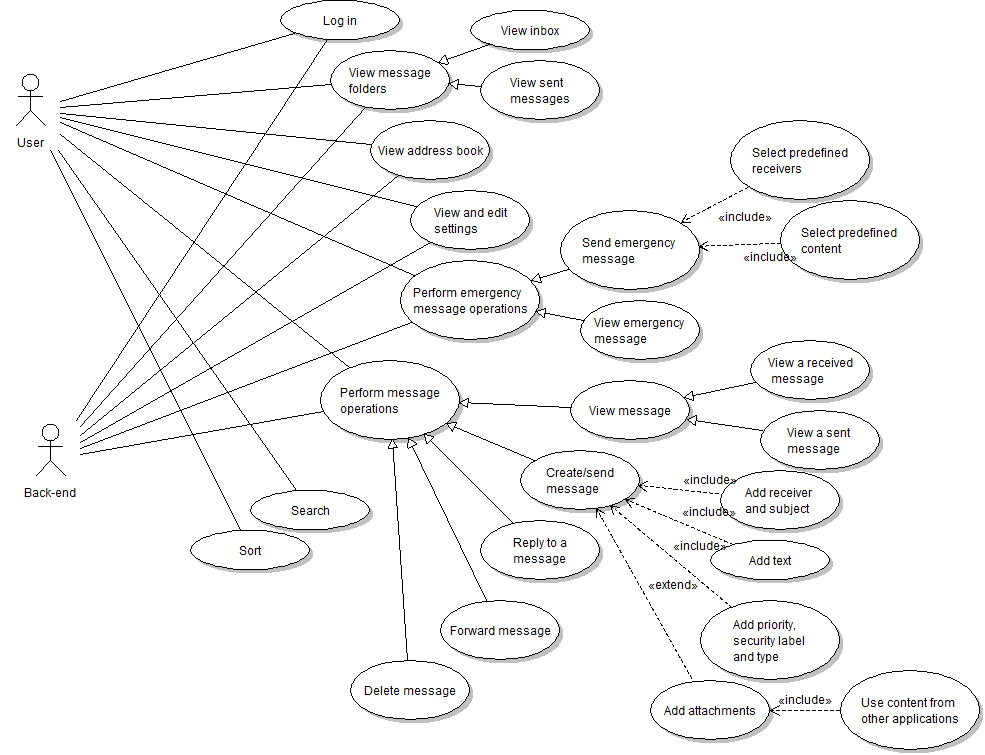
\includegraphics[width=\textwidth]{kpro-use-case}
\caption{Use case diagram} \label{fig:usecase}
\end{center}
\end{figure}

\subsection{Textual use cases}
Each of the use cases is described below, so that the use case diagram will be easier to understand. See table \ref{tab:viewmessages} - \ref{tab:settings} starting at page \pageref{tab:viewmessages} for a more detailed explanation of the use cases.


\begin{table}
\begin{tabular}{p{3cm}p{12cm}}
& 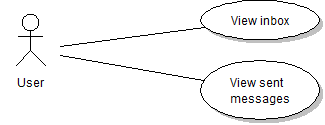
\includegraphics{view_messages}\\ \hline
Element & Description \\ \hline
Use case name & View messages \\
Goal & View received and sent messages \\
Summary &The user would like to view received and sent messages \\
Preconditions &
\begin{enumerate}
\item{}The application is running.
\item{}The user is logged in.
\end{enumerate} \\ \hline
Flow of Events &
\begin{enumerate}
\item{}The user selects a message from either the inbox or sent messages.
\item{}Message is showed to user.
\end{enumerate} \\ \hline
Exceptions & There are no existing messages.
\end{tabular}
\caption{View messages textual use case} \label{tab:viewmessages}
\end{table}

\begin{table}
\begin{tabular}{p{3cm}p{12cm}}

Element & Description \\ \hline
Use case name & Reply, forward and delete \\
Goal & Reply, forward and delete messages\\
Summary & The user would like to reply to a message, forward it or delete it. \\
Preconditions &
\begin{enumerate}
\item{}The application is running.
\item{}The user is logged in.
\end{enumerate} \\ \hline
Flow of Events &
\begin{enumerate}
\item{}The user selects a message from either the sent or inbox messages.
\item{}Message is showed to user.
\item{}User chooses to reply, forward or delete the message. 
\end{enumerate} \\ \hline
Exceptions & There are no existing messages.
\end{tabular}
\caption{Reply, forward and delete textual use case} \label{tab:viewmessages}
\end{table}

\begin{table}
\begin{tabular}{p{3cm}p{12cm}}

Element & Description \\ \hline
Use case name & View message folders \\
Goal & View inbox and sent messages \\
Summary &The user would like to view the inbox and a list of sent messages \\
Preconditions &
\begin{enumerate}
\item{}The application is running.
\item{}The user is logged in.
\end{enumerate} \\ \hline
Flow of Events &
\begin{enumerate}
\item{}The user enters the inbox or sent messages.
\item{}The list of messages in the inbox or sent messages is presented to the user.
\end{enumerate} \\ \hline
Exceptions & There are no existing messages.
\end{tabular}
\caption{View message folders use case} \label{tab:viewmessages}
\end{table}

\begin{table}
\begin{tabular}{p{3cm}p{12cm}}
& 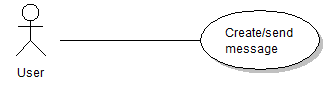
\includegraphics{create_message}\\ \hline
Element & Description \\ \hline
Use case name & Create message \\
Goal & User creates and sends a complete message \\
Summary &The user would like to create/send a message to a receiver with a subject and text. The user would also like to set the priority, security label and type of the message as well as being able to add an attachment from other applications. \\
Preconditions &
\begin{enumerate}
\item{}The application is running.
\item{}The user is logged in.
\end{enumerate} \\ \hline
Flow of Events &
\begin{enumerate}
\item{}User selects new message.
\item{}The user adds the recipient(s) and subject to the message.
\item{}The user sets the priority, security label and type.
\item{}The user adds attachments if needed.
\end{enumerate} \\ \hline
Exceptions & The user does not set priority, security label and type and default values are set.
\end{tabular}
\caption{Create message textual use case} \label{tab:createmessage}
\end{table}

\begin{table}
\begin{tabular}{p{3cm}p{12cm}}

Element & Description \\ \hline
Use case name & Send emergency message \\
Goal & User sends an emergency message \\
Summary & The user sends an emergency message with predefined content to predefined receivers \\
Preconditions &
\begin{enumerate}
\item{}The application is running.
\item{}The user is logged in.
\end{enumerate} \\ \hline
Flow of Events &
\begin{enumerate}
\item{}User selects new emergency message.
\item{}The user sends the message.
\end{enumerate} \\ \hline
Exceptions & The predefined values have not been set.
\end{tabular}
\caption{Send emergency message textual use case} \label{tab:createmessage}
\end{table}




\begin{table}
\begin{tabular}{p{3cm}p{12cm}}

Element & Description \\ \hline
Use case name & View emergency message \\
Goal & User views an emergency message \\
Summary & The user receives and viesw an emergency message \\
Preconditions &
\begin{enumerate}
\item{}The application is running.
\item{}The user is logged in.
\end{enumerate} \\ \hline
Flow of Events &
\begin{enumerate}
\item{}User receives an emergency message.
\item{}A popup appear on the users screen.
\item{}User presses the popup and views the emergency message.
\end{enumerate} \\ \hline
\end{tabular}
\caption{View emergency message textual use case} \label{tab:createmessage}
\end{table}

\begin{table}
\begin{tabular}{p{3cm}p{12cm}}
& 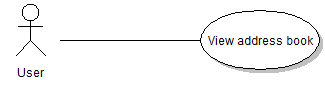
\includegraphics{view_address_book}\\ \hline
Element & Description \\ \hline
Use case name & View and interact with address book \\
Goal & User can view and interact with the address book \\
Summary &The user enters the address book and is able to view, add, edit and delete contacts. \\
Preconditions &
\begin{enumerate}
\item{}The application is running.
\item{}The user is logged in.
\end{enumerate} \\ \hline
Flow of Events &
\begin{enumerate}
\item{}User selects address book.
\item{}User either adds a new contact or selects an existing one.
\item{}If the user selects an existing contact, he can either edit that contact or delete it.
\end{enumerate}
\end{tabular}
\caption{View and interact textual use case} \label{tab:viewandinteract}
\end{table}

\begin{table}
\begin{tabular}{p{3cm}p{12cm}}
& 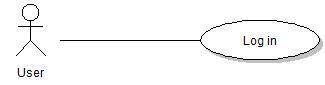
\includegraphics{login}\\ \hline
Element & Description \\ \hline
Use case name & Log in \\
Goal & User logs in with a username and password. \\
Summary &The user is prompted with a login screen and must type in his username and password. \\
Preconditions &
\begin{enumerate}
\item{}The application is running.
\end{enumerate} \\ \hline
Flow of Events &
\begin{enumerate}
\item{}User starts application.
\item{}User is prompted with username and password.
\item{}User types in username and password and presses the login button.
\item{}User gains access to the application data and functionality.
\end{enumerate} \\ \hline
Exceptions & User types wrong username and password and is denied access.
\end{tabular}
\caption{Log in textual use case} \label{tab:login}
\end{table}

\begin{table}
\begin{tabular}{p{3cm}p{12cm}}
& 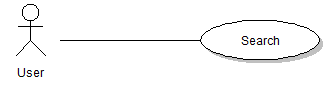
\includegraphics{search}\\ \hline
Element & Description \\ \hline
Use case name & Search \\
Goal & User receives search results for a given search text. \\
Summary & The user search in the application for mail, contacts etc through a search field at the top of the screen. \\
Preconditions &
\begin{enumerate}
\item{}The application is running.
\item{}The user is logged in.
\end{enumerate} \\ \hline
Flow of Events &
\begin{enumerate}
\item{}User highlights search field and inserts his the text he wants to search for.
\item{}User presses the search button.
\item{}Application shows search results to the user.
\end{enumerate}
\end{tabular}
\caption{Search textual use case} \label{tab:search}
\end{table}

\begin{table}
\begin{tabular}{p{3cm}p{12cm}}
& 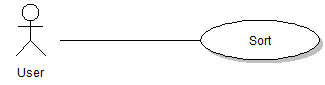
\includegraphics{sort}\\ \hline
Element & Description \\ \hline
Use case name & Sort \\
Goal & User sorts the messages in his inbox. \\
Summary & The user chosoes a value that he wishes the messages to be sorted by. \\
Preconditions &
\begin{enumerate}
\item{}The application is running.
\item{}The user is logged in.
\item{}There are messages to sort.
\end{enumerate} \\ \hline
Flow of Events &
\begin{enumerate}
\item{}The user selects the value he wishes the messages to be sorted by.
\item{}The application sorts the messages and displays them to the user.
\end{enumerate}
\end{tabular}
\caption{Sort textual use case} \label{tab:search}
\end{table}

\begin{table}
\begin{tabular}{p{3cm}p{12cm}}
& 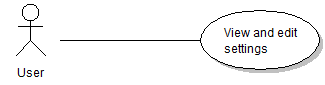
\includegraphics{settings}\\ \hline
Element & Description \\ \hline
Use case name & Settings \\
Goal & The user can alter settings. \\
Summary & The user enters the settings menu and alter the settings to suit his own preferences. \\
Preconditions &
\begin{enumerate}
\item{}The application is running.
\item{}The user is logged in.
\end{enumerate} \\ \hline
Flow of Events &
\begin{enumerate}
\item{}User presses the settings button.
\item{}User alters the settings he wishes to.
\item{}Application saves the alterations.
\end{enumerate}
\end{tabular}
\caption{Settings textual use case} \label{tab:settings}
\end{table}


	%\section{User Stories}

	

\section{Requirements from the customer}

\begin{enumerate}
\item{} \textbf{General functional requirements}
\begin{enumerate}
\item{}The application is to offer a messageservice adapted to mobile users. The application must have a user interface that requires little to no training and is efficient to use.
\item{}Intended users are people who need a reliable and secure communication channel to recieve and send more or less time-critical information. Users are assumed to have acess only to a tablet or phone.
\item{}The applications functions similar to a normal email client, but with a user interface for small devices; sending short messages(at most 500 characters), support for domain-specific attributes, as well as reliability and safety modifications.
\item{}The application must use common standards for Internet Mail to communicate with a XOmail SMTP Gateway. The gateway offers email services based om SMTP(RFC 5321) and SMTP Submit(RFC 4409), Internet Message Format(RFC 5322), SMTP MIXER X.400(RFC 2156), MMHS in Internet Mail(RFC 6477).
\end{enumerate}
\item{}\textbf{Platform}
\begin{enumerate}
\item{}The application should work on an Android-based smartphone or tablet. The user interface should be adapted to the specific screen sizes for these devices, as well as for touch screen.
\item{}The application should be able to work on any network with with bandwidth 64kbps or more.
\item{}The application should be able to communicate via IP networks with a XOmail SMTP Gateway(IMAP/POP3 and SMTP Server).
\item{}The application must work with reduced functionality with a common mail server with IMAP/POP3/SMTP. Functionality that only works against XOmail must be documented.
\end{enumerate}
\item{}\textbf{Message operations}
\begin{enumerate}
\item{}The application should make it possible to communicate bt messages. Messages are to consist of a combination of text, pictures and video.
\item{}Attachments should be retrievable from files stored on the device, or through other applications. For example, it should be possible to take a picture and add it to the message.
\item{}It should be possible to create, edit, send, reply, forward and delete messages. It should also be possible to browse and open received messages.
\item{}The application should support these military attributes from RFC 6477: MMHS-Primary-Precedence, MMHS-Message-Type.
\item{}The application should support safety labeling using the SIO-Label header. The application must support the safety labels below. All messages will have a rating, and it should be possible to configure a default rating.
\begin{itemize}
\item{}Norwegian: UGRADERT(ug), BEGRENSET(b), KONFIDENSIELT(k)
\item{}English(generic): UNCLASSIFIED(u), RESTRICTED(r), CONFIDENTIAL(c)
\item{}NATO: NATO UNCLASSIFIED(nu), NATO RESTRICTED(nr), NATO CONFIDENTIAL(nc)
\end{itemize}
\item{}It should be possible to ask for a delivery report and/or a receipt notification from the message reciever.
\item{}It should be possible to see status of the messages where a delivery report or a receipt notification was asked for.
\item{}It should be possible to send instant messages with a predefined grading and priority to a predefined list of recipients. These may consist of a pre-defined text, and/or information(IE. a picture or current locationGPS) from another application. To send an instant message, it should only be necessary to make up to GUI operations, such as: open application with seperate icon for instant message, select the text, and select the recipient.
\item{}It shouldl be possible to send messages with content created by other applications on the same device.
\end{enumerate}
\item{}\textbf{Sending and receiving of messages}
\begin{enumerate}
\item{}If message sending fails, the user should be notified. The application should automatically attempt to resend the message, and the user should receives a warning.
\item{}Upon receipt of a mesage with priority FLASH or OVERRIDE the user should be notified and the application given focus. The user should be able to see what the message is about(title and perhaps the top text from the attachments). The user should be able to open the message directly.
\item{}The application should support push messages from the server.
\item{}There should not be used bandwidth when the applicatin is not sending or receiving new messages.
\item{}Messages to be sent should be sorted by priority.
\item{}If the user sends a message with priority OVERRIDE, it should take precedence over all other messages. If a message is about to be sent, the transfer shall be canceled and high-priority messages are to be sent first.
\end{enumerate}
\item{}\textbf{Security}
\begin{enumerate}
\item{}Communication with the server is to be encrypted with SSL.
\item{}Messages must be signed with S/MIME when sending.
\item{}S/MIME-signed messages are to be verified upon receiption.
\item{}Private keys for email signing should not be stored in clear text.
\end{enumerate}
\item{}\textbf{Adress book}
\begin{enumerate}
\item{}The application should retrieve any updated address books from the server.
\end{enumerate}
\item{}\textbf{Non-functional requirements}
\begin{enumerate}
\item{}The application must describe the design and implementation of security features, and demonstrate that they are sufficient. These include loging, SSL, signing/verification, priority handling and safety labeling.
\end{enumerate}
\end{enumerate}

%\chapter{Test plan}

	\chapter{Test plan}

This chapter will describe how we plan to test the application, both continuously and at the end of the project. Section 6.1 describes what methods we plan to use to test our code. Section 6.2 describes the different test tools we will use in the project and why these were used. Section 6.3 details the design verification to be carried out. Section 6.4 details the plan for testing functionality and usability of the project. 

\section{Methods and goals for testing}

The main part of project testing will be done as we go along. Using unit tests, each part of the code will be thoroughly tested before it is put together. Larger scale integration and instrumentation tests are done largely the same way, compounded by informal testing by group members. The sending and receiving of messages will be tested using Greenmail, while Mockito is used to handle not yet implemented classes as well as emulator free testing for Android specific classes. All of these tools are described in the section below. Towards the end of the project period, including large parts of the fourth sprint, the focus will shift from producing additional code to finding and repairing bugs. While our plan is vaguely based upon, and in large part inspired by, \gls{ieee829} \cite{bib:ieee} we are too informal about it to be able to use such grand claims. In short, our testing plan is to test each public method both for valid and invalid input, and then run larger scale integration tests between modules.
By using dependency injection and Mockito, we will also be able to test top level modules without testing the building blocks of that module. 
\newline
\newline
The overall goal for the test plan is that every part of our code related to the backend service is tested thoroughly, both for valid and invalid input. Though the same would be good for the frontend,
it is harder to do this automaticly, and therefore it will only be tested whether or the functionality works or not. The optimal goal would be 100\% code coverage, but this is rarely feasible, hence
we will settle for anything between 60-80\%. 
\newline
\newline
In order to ensure the greatest possibility of correctness for our code, each member of the team will be responsible for writing test for their code before it is submitted to our common repository.
Changes in the user interface should also be tested, though if there is no automatic way of doing it, one should tests all functionality related to the changes one have made in the code. 



\section{Test tools}
This section will describe the different test tools we plan to use and sums up with why these tools were selected.
\subsubsection{JUnit}
JUnit is the industry standard for test driven development. It works by creating a separate test method for each method in the class that is to be tested. In this way one can test large portions of code independent of the other code sections. For us, it provides many benefits, especially that most of us have dealt with it before and are familiar with the concept.

\subsection{Cobertura}
Cobertura is a tool for calculating the code covered by our tests, and generate a report based on this. While all other testing tools are automatically run at each build cycle, this is not the case with
Cobertura, which need to be invoked by a seperate command. 

\subsection{Mockito}
Mockito is a simple and elegant \gls{api} for mocking classes. With a few lines of code an unimplemented class can be instructed to provide a valid output, allowing other parts of the code to be tested without concerns.

\subsection{Greenmail}
Greenmail is an open source mail server package for testing in Java. It provides all the server side software needed to test simple sending and receiving of mail without having an actual server. 
It does, however, not support the \gls{pami} IDLE, which in turn forced us to test this feature manually.


\subsection{Why we selected these test tools}
The choice of tools was mainly based on previous experience inside the group, the framework provided by and the demands of the platform. 
\newline
\newline
\gls{junit} was chosen because of our previous experience and the fact that the Android instrumentation framework is based on \gls{junit}. Bundled with Mockito it also gives us the possibility to test otherwise Android dependent modules in a Java environment with the Android specifics mocked up. This can greatly reduce the build cycle time, since the tests no longer need to be pushed onto a device in order to run. Mockito also provides another benefit, in that you can test a component without testing its dependencies. This allows for highly specific testing of just one class, component or module.
\newline
\newline
Greenmail was chosen based on the need to test the message module in our project, ease of use and fast response time. If the code passes the Greenmail tests, the code is then tested against gmail’s mail server to ensure that functions with external servers as well. 


\section{Design Verification}
In order to accommodate the agile development plan used by the team, our early design verification is necessarily somewhat vague. In the early stages of the project we had limited knowledge of how the final product would be structured and which features it would involve.
\newline
\newline
Early in the first sprint we decided upon a set of basic interfaces, which neatly split up the project into manageable parts. We began early by writing up tests for future classes that implemented these interfaces, allowing low level testing of individual methods. At the time of writing these tests we had no idea how each method was going to be implemented. This enabled us to write generic black box tests.
\newline
\newline
Later in the project this method level testing will be augmented by white box and stress testing; essentially us deliberately trying to crash the system with strange inputs or action combinations. 


	
\section{Black-box testing}
		Black-box testing is a software testing method to test the functionality of the program. The tests focus on how the software is supposed to behave, but not how the software does it behind the scenes. The internal of the software is not known to the tester, hence the software can be called a black box. The tester provides input (touch, keystroke etc.) and compare the output to the expected result. Black-box testing is useful in all levels of software testing, from unit testing to acceptance testing, but it becomes increasingly more useful with higher levels. 
%Kilder: http://en.wikipedia.org/wiki/Black-box_testing (09.11)
%Kilder: http://softwaretestingfundamentals.com/black-box-testing/ (09.11)
\newline
\newline
We chose to use two forms of functional testing, namely functional testing and usability testing. 
		\subsection{Functional testing}
			\paragraph{Method}
				Functional testing is a type of black-box testing that is based on test cases derived from the specification of the software. One tests by providing input, as touch or keyboard gestures, and compare the actual to the expected result. 
%Kilder: http://en.wikipedia.org/wiki/Functional_testing (10.11)
			\paragraph{Template for functional testing}		
			The template for functional testing can be found in table \ref{tab:casetemp1} on page \pageref{tab:casetemp1}.	
				\begin{table}
					\begin{tabular}{l|p{10cm}}\hline
						Test case ID & id \\ \hline
						Name & Shortname for the test\\ \hline
						Requirement & Requirement reference\\ \hline
						Description & Description of test\\ \hline
						Preconditions & The conditions of the application before the tests are started\\ \hline
						Flow of events & The list of steps necessary to complete the test \\ \hline
						Expected results & The end result if everything works as expected\\ \hline 
						Actual results & The end result\\ \hline
						Comments & What went wrong, what could been the cause\\ \hline
						Status &OK (no errors), OK- (minor issues) and Failed (not working)\\ \hline
					\end{tabular}
				\caption{Test case template} \label{tab:casetemp1}
			\end{table}
			\paragraph{The tests}
				The test cases 1-25 are meant to verify that the app works correctly to normal use, whereas the test cases 26-28 are meant to that the app behaves well with incorrect input. The test cases can be found in the APPENDIX REFERANSE HER.
			\paragraph{Results}
				A summary of the test results can be found in table \ref{tab:caseresults} on page \pageref{tab:caseresults}.
				\begin{table}
					\begin{tabular}{l|l|l}\hline
						Test case ID &Test name&Result \\ \hline
						1&Login&OK\\
						2&Send regular message&OK\\
						3&Send message to contact from the address book&OK\\
						4&Send full message&OK\\
						5&Sent messages folder&OK\\
						6&Read and browse messages&OK\\
						7&Send attachments (camera)&OK\\
						8&Send attachments (gallery)&OK\\
						9&Send attachments (GPS)&OK\\
						10&Attachments received&OK\\
						11&Instant message settings&OK\\
						12&Message retrieval strategy settings&Failed\\
						13&Security labels settings&Failed\\
						14&Send instant message&OK\\
						15&Receive flash/override message&OK\\
						16&Send instant message with attachments&GPS failed, images OK\\
						17&Receive instant message outside the app&OK\\
						18&Widget for instant message&OK\\
						19&Reply&OK-\\
						20&Forward&OK-\\
						21&Delete&Failed\\
						22&Delivery report and receipt notification&Failed\\
						23&Status of delivery report and receipt notification&Failed\\
						24&Sort messages&OK\\
						25&Search in inbox&Failed\\	
						26&Login incorrect input&OK\\
						27&Receiver incorrect input&OK\\
						28&Security label incorrect input&OK\\ \hline
					\end{tabular}
				\caption{Functional test result summary} \label{tab:caseresults}
			\end{table}
			\paragraph{Discussion}
			The results from the functional testing showed that 19 out of the 28 test cases passed the test,  six failed and three almost passed. Out of the six that failed, three were due to not having time to start with the implementation and three were known bugs that we did not get the time to fix. The three that almost passed were issues that we know how to fix but had not seen until the test.
	\subsection{Usability testing}
		\paragraph{Method}
			Usability testing is testing of the app on possible end-users. This is also a kind of black-box testing meant to observe how users use the app to find unknown errors and get an evaluation of the design and usability of the app. We created a test with six cases that mirrored the most important actions in the app. The test persons tried to solve the tasks while the test leaders measured the time spent on each task and noted problems/comments/thoughts. After the test the persons filled out a SUS form.
\paragraph{SUS}
SUS is an abbreviation for System Usability Scale and is a simple Likert scale of ten questions where the test persons shall give a score from 1 to 5 where 1 is strongly disagree and 5 is strongly agree. The purpose is to obtain a global view of subjective evaluation of the usability of the software.
%Kilde: http://en.wikipedia.org/wiki/System_usability_scale (12.11)
\newline
\newline
			The SUS score is calculated in the following way:
				\begin{enumerate}
					\item{}Take the odd numbered questions and subtract 1 from these scores.
					\item{}Take the even numbered questions and subtract the score from 5.
					\item{}Add these scores together. 
					\item{}Take this sum and multiply by 2.5.
					\item{}Then you have a SUS score between 0 and 100.
				\end{enumerate}
		\paragraph{Usability goals}
		Before conducting the usability tests, we set some usability goals, to have something to assess the usability against.
		\begin{enumerate}
			\item{}The users should not spend more than 5 minutes on a task.
			\item{}The app should not crash during the usability tests.
			\item{}The users should not make more than 1 error during the tasks
			\item{}The users should solve task 6 faster than task 1 (memorability)
			\item{}The average SUS score should be above 70 FOOTNOTE?
		\end{enumerate}
		\paragraph{Templates}
			SUS form REFERANSE TIL APPENDIX
			\newline\newline
			Observation form REFERANSE TIL APPENDIX
		\paragraph{The tests}
			We had five persons perform the tests. The reason behind this number is the theory of Jakob Nielsen SOURCE, who states that a test with five persons should discover about 85 \% of the usability problems. This approach suggested that we should test and redesign three times, but due to time constraints we did not conduct more than one iteration.  
% Kilde: http://www.useit.com/alertbox/20000319.html (12.11)
		\newline \newline
		The tests can be found in table \ref{tab:usabilitytask1} - \ref{tab:usabilitytask6} on page \pageref{tab:usabilitytask1} - \pageref{tab:usabilitytask6}.
		\begin{table}
			\begin{tabular}{>{\bfseries}l l}	
				Task no.&1\\ \hline
				Task name&Log in\\ \hline
				Description&Log in to the app with username and password\\ \hline
				Input&Username="kprotesting" \\
					&Password="kprotest"\\ \hline
			\end{tabular}
			\caption{Usability test - task 1} \label{tab:usabilitytask1}
		\end{table}
		\begin{table}
			\begin{tabular}{>{\bfseries}l l}	
				Task no.&2\\ \hline
				Task name&Send message\\ \hline
				Description&Send a regular message\\ \hline
				Input&To="kprothales@gmail.com" \\
					&Subject="Usability test"\\
					&Security label="UNCLASSIFIED"\\ 
					&Priority="Routine"\\
					&Type="Operation"\\
					&Message text=Enter your own text here\\ \hline
			\end{tabular}
			\caption{Usability test - task 2} \label{tab:usabilitytask2}
		\end{table}
		\begin{table}
			\begin{tabular}{>{\bfseries}l l}	
				Task no.&3\\ \hline
				Task name&Settings\\ \hline
				Description&Change the settings for predefined attributes for instant message\\ \hline
				Input&Standard receiver="kprotesting@gmail.com" (yourself)\\
					& Security label="RESTRICTED",\\
					&Priority="Flash"\\
					& Type="Drill"\\ \hline
			\end{tabular}
			\caption{Usability - test task 3} \label{tab:usabilitytask3}
		\end{table}
		\begin{table}
			\begin{tabular}{>{\bfseries}l l}	
				Task no.&4\\ \hline
				Task name&Send instant message with attachments\\ \hline
				Description&Send instant message with an image\\ \hline
				Input &Image=Take one with the camera\\
					&Message text=Enter you own text here\\ \hline
			\end{tabular}
			\caption{Usability test - task 4} \label{tab:usabilitytask4}
		\end{table}
		\begin{table}
			\begin{tabular}{>{\bfseries}l l}	
				Task no.&5\\ \hline
				Task name&Read high-priority message with attachments\\ \hline
				Description&Open a received high-priority message and view the attachments\\ \hline
				Input&\\ \hline
			\end{tabular}
			\caption{Usability test - task 5} \label{tab:usabilitytask5}
		\end{table}
		\begin{table}
			\begin{tabular}{>{\bfseries}l l}	
				Task no.&6\\ \hline
				Task name&Send message to a contact from the address book\\ \hline
				Description&Send message to a contact by choosing from from the address book\\ \hline
				Input&To="kprothales@gmail.com"\\
					&Security label="UNCLASSIFIED"\\ \hline
			\end{tabular}
			\caption{Usability test - task 6} \label{tab:usabilitytask6}
		\end{table}
			
		\paragraph{Results}
			The results from the tests can be found in table \ref{tab:usabilitytestresults} on page \pageref{tab:usabilitytestresults}.
			\begin{table}
			\begin{tabular}{l|l|p{8cm}}	\hline
				\textbf{Goal}&\textbf{Status}&\textbf{Comment}\\ \hline \hline
				1&OK&-\\ \hline
				2&Failed&The app crashed in the settings task on almost all tests\\ \hline
				3&OK&One user sent a regular message instead of an instant message\\ \hline
				4&Failed&Two users spent the same amount of time, but this could also be due to the fact that the test leaders here just counted whole minutes\\ \hline
				5&OK&The average SUS score was 78.5\\ \hline 

			\end{tabular}
			\caption{Usability test - Test results} \label{tab:usabilitytestresults}
		\end{table}

			\subparagraph{SUS scores}
			 	\begin{table}
			\begin{tabular}{p{8cm}|l|l|l|l|l|l}	\hline
				\textbf{Question/Test}&\textbf{1}&\textbf{2}&\textbf{3}&\textbf{4}&\textbf{5}\\ \hline \hline
				1. I think that I would like to use this system frequently&3&3&4&4&3\\ \hline
				2. I found the system unnecessarily complex&2&2&2&1&2\\ \hline
				3. I thought the system was easy to use&4&4&4&5&4\\ \hline
				4. I think that I would need the support of a technical person to be able to use this system&1&2&1&1&1\\ \hline
				5. I found the various functions in this system were well integrated&3&3&3&5&5\\ \hline
				6. I thought there was too much inconsistency in this system&2&2&2&3&1\\ \hline
				7. I would imagine that most people would learn to use this system very quickly&4&3&4&4&4\\ \hline
				8. I found the system very cumbersome to use&3&2&2&1&1\\ \hline
				9. I felt very confident using the system&4&4&4&4&5\\ \hline
				10. I needed to learn a lot of things before I could get going with this system&1&2&1&1&1\\ \hline \hline
				\textbf{Score}&\textbf{72.5}&\textbf{67.5}&\textbf{77.5}&\textbf{87.5}&\textbf{87.5}\\ \hline 
				
			\end{tabular}
			\caption{Usability test - SUS scores} \label{tab:usabilitysusscore}
		\end{table}
			The SUS results are shown in table \ref{tab:usabilitysusscore} on page \pageref{tab:usabilitysusscore}.
			\newline\newline
			\subparagraph{Time spent}
				\begin{table}
			\begin{tabular}{l|l|l|l|l|l|l|l}	\hline
				\textbf{Task/Time}&\textbf{1}&\textbf{2}&\textbf{3}&\textbf{4}&\textbf{5}&\textbf{Average}\\ \hline \hline
				1&1 min&1 min&1 min&1 min&1 min&\textbf{1 min}\\ \hline
				2&3 min&3 min&2 min&2 min&2 min&\textbf{2.4 min}\\ \hline
				3&3 min&4 min&4 min&5 min&5 min&\textbf{4.2 min}\\ \hline
				4&1 min&5 min&2 min&3 min&4 min&\textbf{3 min}\\ \hline
				5&1 min&1 min&0 min&2 min&3 min&\textbf{1.75 min}\\ \hline
				6&1 min&2 min&1 min&2 min&2 min&\textbf{1.6 min}\\ \hline
				\textbf{Sum}&\textbf{10 min}&\textbf{16 min}&\textbf{10 min}&\textbf{15 min}&\textbf{17 min}&\textbf{14 min}\\ \hline 
				
			\end{tabular}
			\caption{Usability test - Task times} \label{tab:usabilitytasktime}
		\end{table}
			A summary of the time spent on the different tasks is shown in table \ref{tab:usabilitytasktime} on page \pageref{tab:usabilitytasktime}.
			\subparagraph{Observation forms}
			REFERANSE TIL APPENDIX
		\paragraph{Summary}
			There were many problems that reoccured in the test results. Below is a short summary of what were the problems:
			\begin{itemize}
				\item{}The testers were annoyed that the application does not remember login information
				\item{}Some were confused by odd choices of words
				\item{}The testers were annoyed that tilting of the phone sets you back to the inbox
				\item{}Almost all complained that the instant message and settings tab icons were not intuitive and spent some time finding the right tab.
				\item{}Some complained about small fonts and small toasts.
				\item{}Many were annoyed that the text boxes behaved weird, e.g. that the letters were not capitalized after a period and the keyboard did not always close. 
				\item{}The settings were unstable and the app stopped during the task that tested the settings.
				\item{}Many of the testers complained about the lack of confirmation after actions in the app.
				\item{}Some testers commented that the user interface was not pretty enough.
			\end{itemize}
		\paragraph{Discussion}
Even though we did not have the time to make major changes and improvements to the user interface and functionality, we learned a lot from these usability tests about how to better do things in later projects.
		\paragraph{Redesign}
		We were able to do some minor changes in the user interface. The changes are listed below, although some of the screenshots other places may not be updated accordingly.
		\begin{itemize}
			\item{}Hopefully more intuitive icon for instant message. (kanskje de to bildene her?)
			\item{}Implemented bigger difference between read and unread messages in the inbox folder.
			\item{}Text fields give you capitalized first letter of sentences.
			\item{}Rephrased some text, e.g. "username" instead of "email".
		\end{itemize}

%\chapter{Architectural description}
	
	\chapter{Architectural description}
	This chapter will revolve around the final architecture of the prototype created during this project. In our definition of architecture, will have choosen to follow the definition carved out by
	Len Bass, Paul Clements and Rick Kazman. ``The software architecture of a program or computing system is the sructure of structures of the system, which comprise software elements, the externally visible properties of those elements, and the relationships between them''\cite[p. 3]{bib:archi}
	
\section{Architectural Drivers}
	From the nature of the assignment and the requirements received from the customer, we decided that Security had to be one of our quality attributes. After the first couple of meeting with the customer, it became clear that usability also was something of interest to them, and we decided to add Usability to our quality attributes as well. It should however be noted that	all of the quality attributes specified in Len Bass's book 'Software Architecture in Practice'\cite{bib:archi} had their place within this project. Especially Modifiability was one of those that, though not of out main attributes, was given a fairly large amout of consideration in order to ease development at later stages of the project. The reason as to why Modifiability was not one of our main attributes comes down to the expected lifespan of the prototype, which in this case comes down to the success of the project, and what conclusions the customer sees when presented with the final prototype and documentation. However, the project revolves around making a prototype and documenting the steps taken to complete that process, and it is therefore safe to assume that the lifespan of the prototype will be relatively short. 

\section{Architectural viewpoints}
The ``4+1 view model''� \cite{bib:vm} by Philippe Kruchten suggest four different views, logical, process, development and physical. In the case of XOXOmail we are going to use the logical, process and development view. The rationale behind removing the physical view is that XOXOmail will run on a single physical device and only utilize one process, a security view, describing the layers of security, will be added instead.

\subsection{Development view (Subsystem decomposition)}
The development view is a step up from the logical view and focuses on software modules instead of classes. These subsystems/modules are organized in a hierarchy of layers where each layer provides a well-defined interface to layers above. ``The complete development architecture can only be described when all the elements of the software have been identified. It is, however, possible to list the rules that govern the development architecture: partitioning, grouping, visibility'' \cite{bib:vm}. 
Figure \ref{fig:developmentview} at page \pageref{fig:developmentview} shows the Backend Service Connects to all parts of our app. The main focus of this view is to show that it is also the connector to the external part of the app, the SMTP Gateway. This gateway is implemented by Thales, and all we have to do is connect to it using well known protocols.

\begin{figure}[H]
	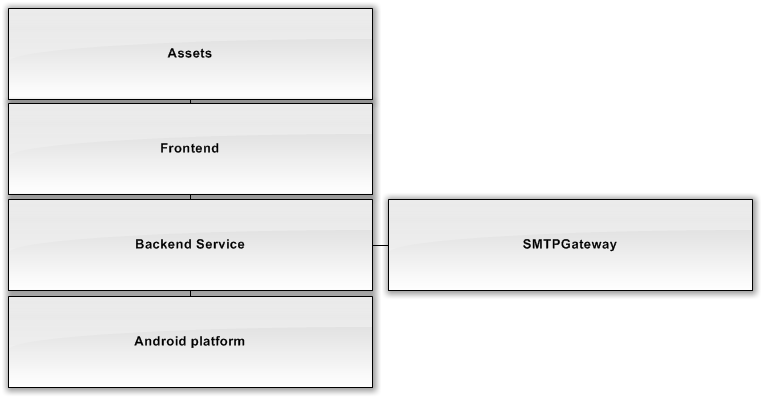
\includegraphics[width=\textwidth]{developmentview.png}
	\caption{Development View}
	\label{fig:developmentview}
\end{figure}

\subsection{Logical view (Object oriented deomposition)}
``The logical architecture primarily supports the functional requirements --- what the system should provide in terms of services to its users. The system is decomposed into a set of key abstractions, taken from the problem domain, in the form of objects or object classes''\cite{bib:vm}. A common way to represent this view is with a class diagram that shows a set of classes and their relationships, we have however used a slightly modified varient, in order to make all the figures more readable.\newline\newline
	\subsubsection{Backend}
\begin{figure}[H]
	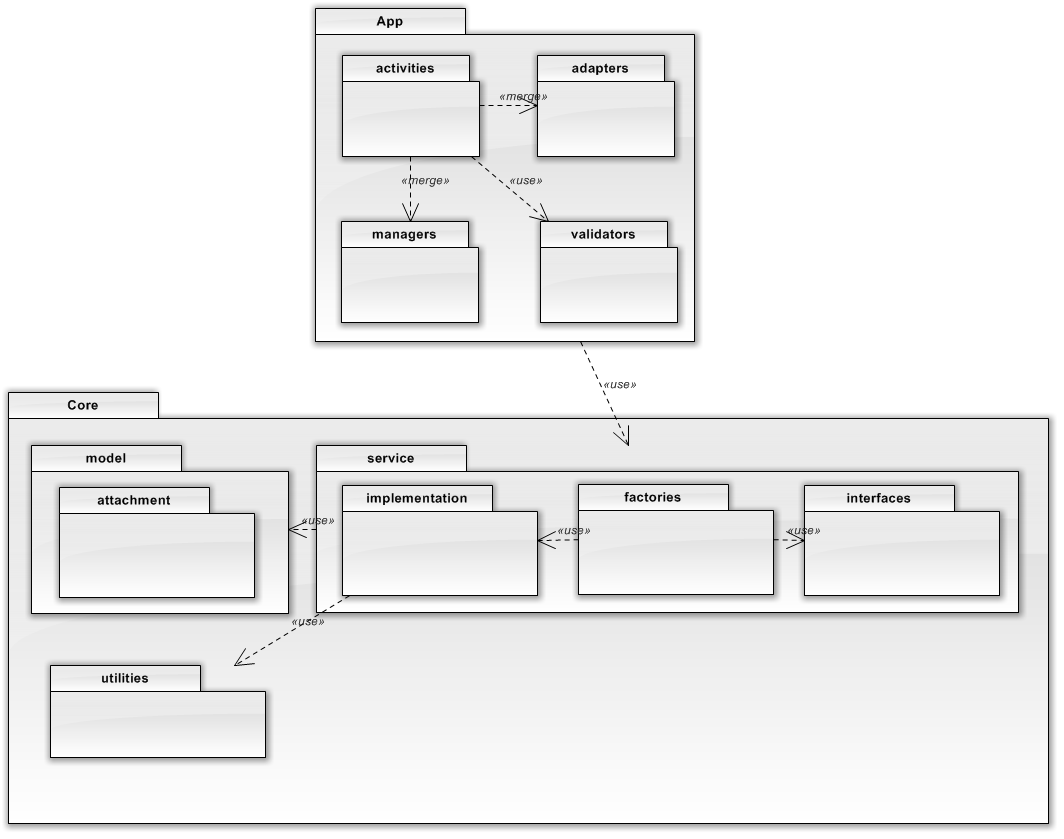
\includegraphics[width=\textwidth]{packageDiagram.png}
	\caption{The logical package view of the architecture}
	\label{fig:logicalpackview}
\end{figure}
Figure \ref{fig:logicalpackview} shown at page \pageref{fig:logicalpackview}, shows a package overview over the project backend. Though very generic, it shows the basic structure of the architecture, and the communication paths between packages. On thing to note, is that in order to add a new service to the architecture, one would need to implement three different objects, a factory for creating the service, an interface describing the service, and the service implementation itself. In the case of XOXOmail, we planned out four different services, the \textit{NetworkService}~(Fig.~\ref{fig:logicalnetworkpackview}~p.~\pageref{fig:logicalnetworkpackview}), \textit{PersistenceService}~(Fig.~\ref{fig:logicalpersistencepackview}~p.~\pageref{fig:logicalpersistencepackview}), \textit{HALService} and \textit{SecurityService}. The two latter was though never used, and their diagrams are therefore omitted here, alongside the diagram for our \textit{Utiliteis} class. The structure of our models can be seen in figure~\ref{fig:logicalmodelpackview} at page \pageref{fig:logicalmodelpackview}

\begin{figure}[H]
	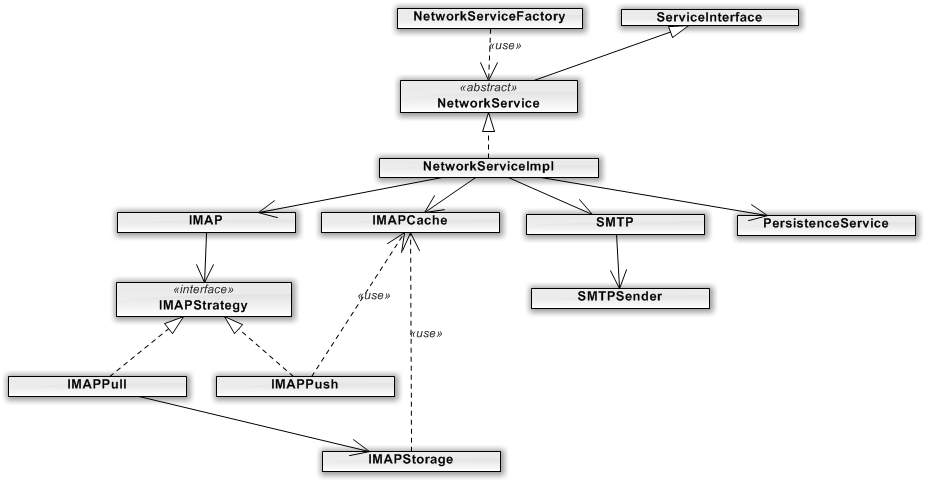
\includegraphics[width=\textwidth]{NetworkService.png}
	\caption{The logical view of the NetworkServicePackage}
	\label{fig:logicalnetworkpackview}
\end{figure}
\begin{figure}[H]
	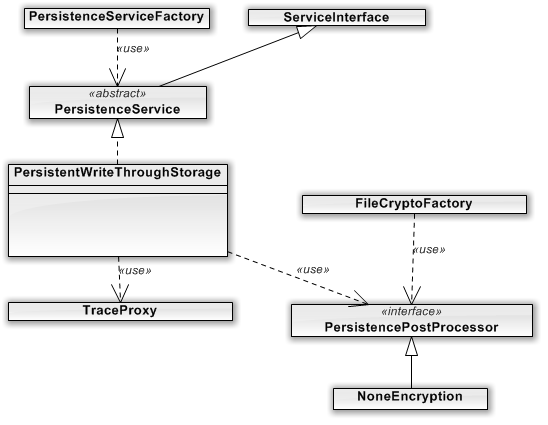
\includegraphics[width=\textwidth]{persistenceService.png}
	\caption{The logical view of the PersistenceService}
	\label{fig:logicalpersistencepackview}
\end{figure}
\begin{figure}[H]
	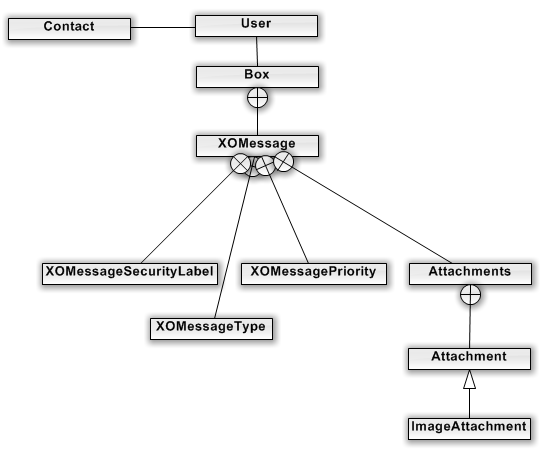
\includegraphics[width=\textwidth]{modelPackage.png}
	\caption{The logical view of the model package}
	\label{fig:logicalmodelpackview}
\end{figure}

The intended purpose of each of the different services is somewhat given by their respective names, but in order to avoid any ambiguity there will be a short recap of their purpose.
\begin{description}
	\item[NetworkService] The \textit{NetworkService}'s reponsebility is to provide the core functionality of sending and receiving mail. 
	\item[PersistenceService] The \textit{PersistenceService}'s responsebility is to keep track of objects being changes, and reflect these changes in a persistent way in case of system failure, or the application is shut down. 
\end{description}

\subsubsection{Frontend}
	\begin{figure}[H]
		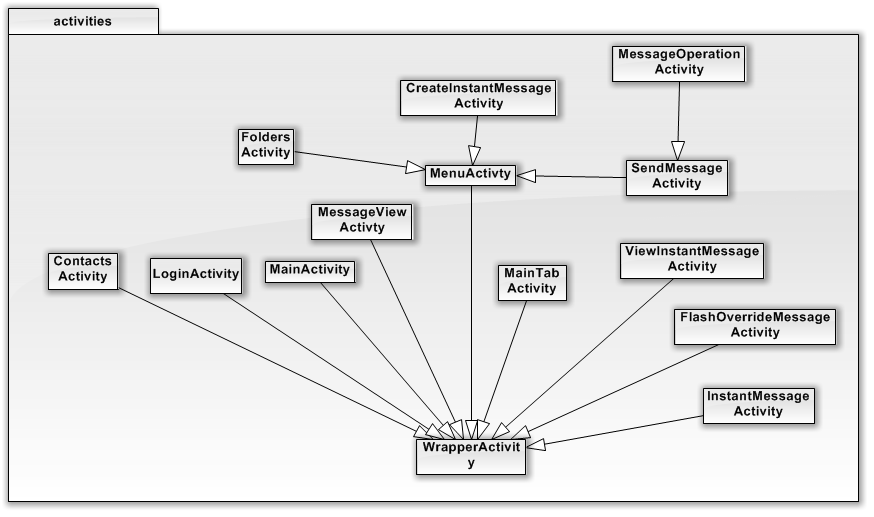
\includegraphics[width=\textwidth]{FrontendClasses.png}
		\caption{The logical view of the frontend activities package}
		\label{fig:logicalfrontpackview}
	\end{figure}	
	
\subsection{Process View}
The process view is concerned with how different tasks bind together to form one executable unit. More specifically, the communication between threads/processes and on which thread/process is a task executed. We will differentiate between major and minor tasks, where major tasks are architectural elements open through a public interface, and minor tasks being tasks introduced in order to implement some functionality in one class or module.
In figure \ref{fig:processview} at page \pageref{fig:processview}, you can differentiate between minor and major tasks by looking at the \textit{SMTP} branch of \textit{NetworkService}, here \textit{SMTPSender} is a minor task, while both \textit{SMTP} and \textit{NetworkService} is considered major tasks. 

\begin{figure}[H]
	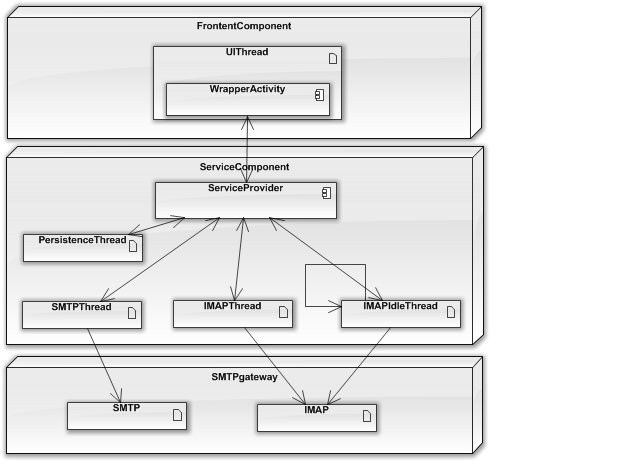
\includegraphics[width=\textwidth]{processview.png}
	\caption{Process view}
	\label{fig:processview}
\end{figure}

One thing to note about the communications paths is that all communication between the \textit{frontent component} and \textit{service component} is between two wrapper classes, \texit{WrapperActivity} at the frontend, and \textit{ServiceProvider} at the backend. 

\subsection{Security View}
The security view is concerned with how the system as a whole is secured. This involves intercommunication, storage and communication with external sources. The view is not however concerned about implementation, just the layers of security.
See figure \ref{fig:securityview} at page \pageref{fig:securityview}.

\begin{figure}[H]
	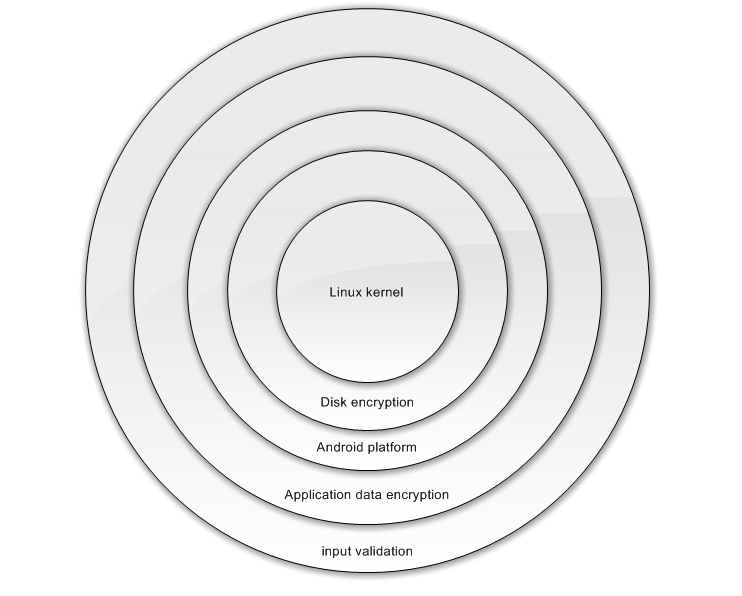
\includegraphics[width=\textwidth]{securityview.png}
	\caption{Security view}
	\label{fig:securityview}
\end{figure} \hfill
\newline
\newline
\textbf{The Linux kernel} provides us with a user-based permissions model and process isolation, which ensures that another process cannot access the memory of XOXOMail during runtime.
\newline
\newline
\textbf{Disk encryption}, is feature provided by the android platform, which encrypts the whole Android device using \gls{aes} with \gls{cbc} and \gls{essiv2}.\cite{bib:crypto}
\newline
\newline
\textbf{Android platform}, most of the security provided by the Android platform is provided by the Linux kernel, but not necessary used in normal conditions. The application sandbox is one of these things. And since the sandboxing operation is located at kernel level, it is hard to break out of. 
\newline
\newline
\textbf{Application data encryption} is a response to the possibility of rooted devices. Normally an android application will not run with root access on the device, this however is not the case on rooted devices. In which case the application and user will have full access to all applications and all application data. By adding our own encryption layer with the key stored off-device we can ensure data security even with root access to the phone\cite{bib:tech}. The encryption we opted for is an \gls{aes} based encryption with a user-password derived key by \gls{pbsha}.
Regarding communication with external resources as a mail-server, it will be done over a secure communication channel providing \gls{ssl1} or \gls{tls}. 
\newline
\newline
\textbf{Input validation} is always necessary in order to provide a secure service. All input to the XOXOMail application should be validated, this is includes received mail, user-input etc. For mail validation we are going to use \gls{emims} signing and verification provided by bouncycastle. 

\section{GUI}

\subsection{Introduction}
The Android platform specifies a certain way of organizing the application, which we have tried to follow.

\subsection{External resources}
The user interface elements, ranging from whole screens (called layouts) to the structure and look of a single list element, are defined in \gls{xml} (Extensible Markup Language) and stored external to the application. An Android project contains a folder named “res” where all external resources are placed. User interface elements are stored in a sub folder called “layouts”. Other resources, e.g. colors or images, are stored inside separate sub folders. The advantage of declaring the user interface and other resources in \gls{xml} is that it enables decoupling of the presentation of the application and the code that controls the application.
\newline
\newline
All resources must be assigned an \gls{id} if they are to be referenced in the application code. All resource \gls{id}s are defined as public constants in the project's R.class, which is a class that is automatically generated during build and contains subclasses for the types of resources where we have defined at least one resource, e.g. R.layout (for user interface elements) or R.color (for definition of colors). The resources can be referenced both inside other resources and in the application code.
\newline
\newline
We also want to use styles, which are collections of properties specifying the look of a layout or a component. It can be compared to the mindset of \gls{css}, where one separate design and content. We might also consider using a theme for our application, which is a style applied to an entire activity or application. The reason behind using styles and themes would be to ensure consistent appearance across the application. 

\subsection{Activities}
Activities are components that provide a screen that the user can interact with, and are classes written in Java. Each activity has a window where the user interface is drawn. One activity is specified as the main activity and is the start screen of the application. Each activity can start another activity to perform different actions. The activities inflate the \gls{xml} layouts to form the user interface and controls the behaviour of the elements. It is also possible to create layout elements programmatically, but we have chosen not to do this as we want the decoupling mentioned above.
\newline
\newline
An activity is always in one of four possible states \cite{bib:aas}:
\begin{itemize}
\item{}Active/running: When the activity is in the foreground of the screen
\item{}Paused: When the activity has lost focus but is still visible
\item{}Stopped: When the activity is completely obscured by another activity
\item{}If an activity is paused or stopped, it is likely that the system asks the activity to finish or just kill its process, hence drops it from memory. It then has to be restarted completely.
\end{itemize}

The life cycle of an activity can be seen in figure \ref{fig:lifecycle} at page \pageref{fig:lifecycle}.
\begin{figure}
	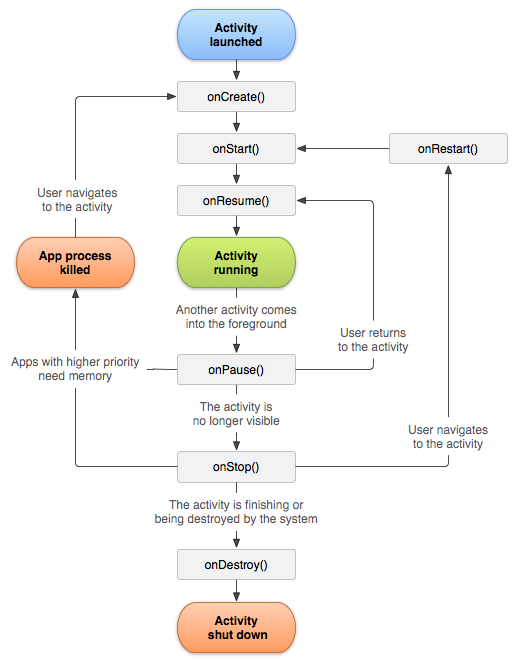
\includegraphics[width=\textwidth]{activity_lifecycle}
	\caption{Activity life cycle \cite{bib:alc}}
	\label{fig:lifecycle}
\end{figure}

All the methods starting with on (onCreate etc.) can be overwritten to administrate what the application should do in the changes of state.

\paragraph{How we did it in our app}

\begin{figure}
	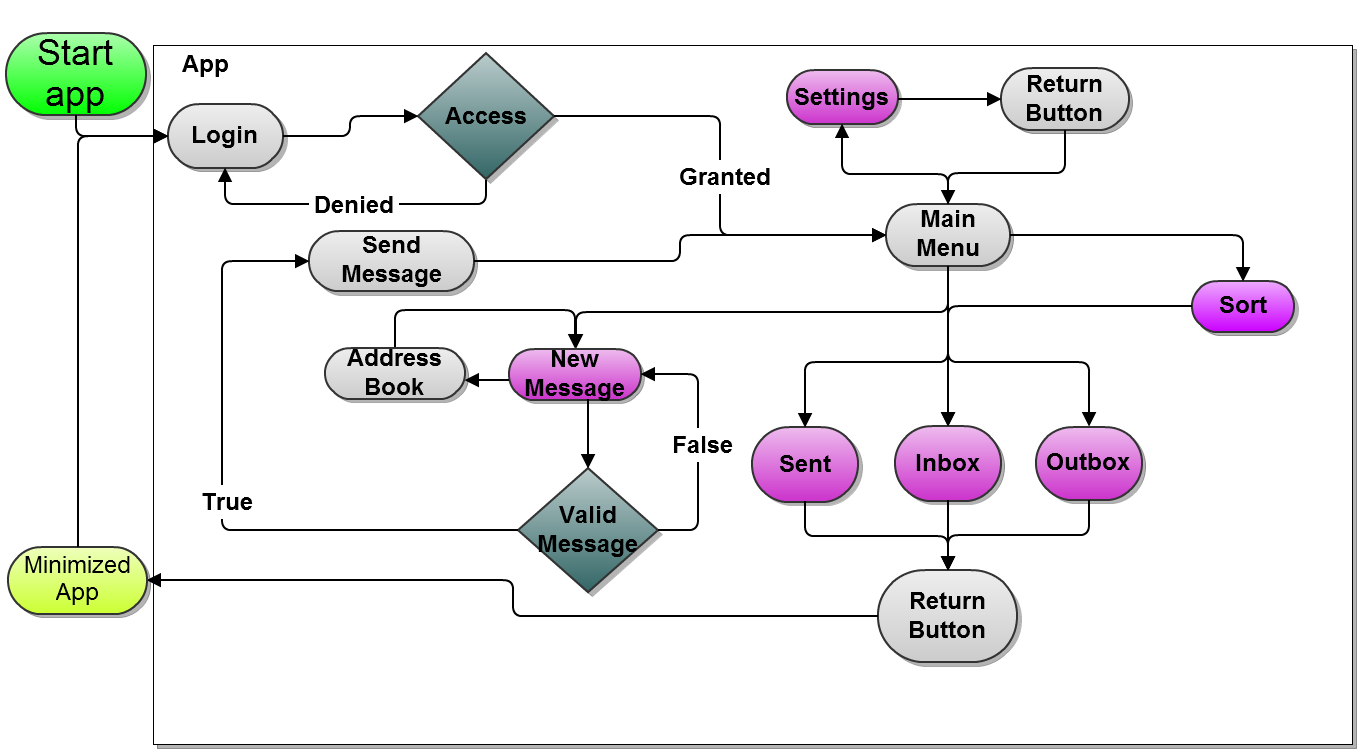
\includegraphics[width=\textwidth]{Android_GUI_flow_chart_2}
	\caption{The logical view of the GUI architecture}
	\label{fig:logicalGUIview}
\end{figure}

Figure \ref{fig:logicalGUIview} at page \pageref{fig:logicalGUIview} shows the flow in our app. It all starts in the upper left corner at "Start app". The first activity you see is the \textsc{Login Activity}. The user is granted access if a correct username and matching password is entered. He is then sent directly to the main menu, where he can choose to either see messages, send a new message or alter settings. Which messages are shown are based on if you choose \textsc{Sent}, \textsc{Outbox} or \textsc{Inbox}. By pressing \textsc{Sort} he can choose to alter the way the messages are shown. Choosing to send a message can either be done by going into the regular send message view, or the instant message view. Either way, for a message to be sent, it has to be validated. When all fields are valid, the message is sent to the correct recipient. By pressing return button when inside app we are minimizing the app. It will still be running in the background.

\subsection{The Android manifest}
The Android manifest \cite{bib:aman} is what binds the applicaiton together. It is defined in \gls{xml} and details the structure and metadata of the application, its components and requirements. The manifest needs to have nodes for each of the components, which in our case are activities and services. Relevant metadata is the application name, icon and theme. The manifest also declares the permissions the application needs to access protected parts of the \gls{api} and interact with other applications.

\subsection{Supporting different hardware and internationalization}
By conforming to using external resources on can easily build applications that support differences such as varying screen sizes and languages. For example, it is possible to create a low, medium and high dpi (dots per inch, a measure of screen density) version of an image and Android will select the correct version based on the screen size. Android can pick layouts based on the screen orientation, where the possibilities are that the phone is an portrait or landscape mode. It is also possible to have Android decide what language to use based on location, but this is not relevant to this project. 

	 \subsection{Fulfillment of requirements}

\subsubsection{Functional quality requirements}
All of the functional requirements listed in section ??? (Business requirements sec.1@googledocs), require two things from the application and architecture, a frontend graphical user interface for the user to interact with, and backend service providing the frontend with data and functionality. The fulfillment of functional requirement will therefore not be investigated any further.

\subsubsection{Non-functional quality requirements}

\paragraph{Usability}
The architecture has in no way changed due to the usability requirements. 

\paragraph{Security}

\subparagraph{Accessing locally stored data outside of app}
“No data exposed to the user or app, as long as the user do not have root access.” S1 - Quality requirements
\newline
\newline
This requirement is fulfilled by the PersistenceImpl, (figure in graphical view of architecture), which keeps track of all the models currently in use in the application. If the malicious user or application does not have root access, then the data will be secure just by using android provided features like sandboxing processes and private storage. We can not however guarantee that this will always be the case, and another layer of security is therefore needed. 
\newline
\newline
There are two possible scenarios when looking at this requirement. First off, a malicious user/application find a locked/encrypted device, where the owner is not logged in to the device. In this case, the android hardware encryption will successfully mitigate any malicious intent.
Secondly, a malicious user/application find a unlocked devices, but the owner is not logged into the XOXOMail. Under normal circumstances, without an additional layer of security, the malicious user could gain access to the application and application data, circumventing the android private storage access control due to the users root privileges. In order to mitigate this, all XOXOMail specific data will be encrypted before stored into the private storage section. 
Third, a malicious user/application find an unlocked device, where the owner is logged into the XOXOMail application. In this case the malicious user is given some possible ways of exploiting the application by sending predefined flash messages. But it would still require the malicious user to type in the owner password in order to browse any other messages. 

\subparagraph{Trying to use app with wrong privileges}
“No features exposed to the user - stopped by login screen” S2 - Quality requirements
\newline
\newline
This requirement is fulfilled by the ServiceProvider along with the graphical user interface. There are two possible scenarios when looking at this requirement. First off, the service backend is not started and a user starts the app. In this case the no privileges will be given until the user types in the correct username and password. In fact, the application itself does not have the possibility to decrypt any data without this information.
	Secondly, the service is started, but not open. In this case a malicious user could send predefined flash messages, but not view any messages, or get access to the system as a whole. 

\subparagraph{Trying to access the apps external data trafic}
“No useful data exposed to the user” S3 - Quality requirements
\newline
\newline
This requirement is fulfilled by the third party library, JavaMail, which ensures a secure communication channel to the mail server. JavaMail  will setup a SSL/TLS connection, mitigating the possibility of looking into the data traffic generated by the application.

\paragraph{Performance}

\subparagraph{Latency}
“With a latency of maximum 3 seconds, the user should be able to read the message after it is received. This is the latency when we subtract the download time of message, which is dependent of the network connection.” P1 - Quality requirements
\newline
\newline
This requirement is fulfilled by the IMAPIdle module, (figure in graphical view of architecture), which keeps an open connection from the device to the IMAP server. The IMAP server will not respond to the IDLE request until a new message is received or a message is deleted. Once the client receives an answer from the server it can determine the correct course of action and issue a new IDLE request, causing it to go back into a waiting stage. 

\part{Scrum process}

%\chapter{Product backlog}

	\section{Product Backlog}

%\chapter{Sprint 1}

	\chapter{Sprint 1}

\section{Sprint 1 - Overview}
The time leading up to Sprint 1 was spent looking into different solutions and agreeing on details such as programming language, development tools and top level architecture. We also spent a large part of the week setting up various tools on our personal computers; especially accounting for the wide variety of hardware and operating systems.
\newline
\newline
Sprint 1 was our first major coding spree. We set aside some time to set up all the required software and communications on the last few computers, but most of the time was to be spent putting together a rough prototype. Our goal was to be able to send and receive messages from the phone by the end of the sprint, providing us with a functional framework we could bolt our later expansions on to. Tasks like security and intuitive GUI were saved for later sprints.
\newline
\newline
As well as the coding, which was to be largely handled by three of us in this first sprint, a lot of time was scheduled for theoretical studies. Things to be implemented later had to be researched and documented, and lot of basic things like agenda templates and documentation structure had to be set up.

	\section{Sprint 1 - Concrete project work plan}

\textbf{Milestone:} Have a working demo to show the customer and adviser that is able to send and receive messages, as well as open old messages. We want to have a GUI that is functional but not necessarily pretty or finalized.
\newline
\newline
See table \ref{tab:sprint1tasks} at page \pageref{tab:sprint1tasks}.
\newline
\newline
Explenations of the short names in the table:\\
KP-10: Meetings \\ 
KP-54: Create interfaces between Core and GUI \\
KP-75: Starting App \\
KP-76: Sending a message\\
KP-77: Persisting data to phone
\begin{table}
\begin{tabularx}{\linewidth}{>{\setlength\hsize{.2\hsize}}X|>{\setlength\hsize{1.5\hsize}}X|>{\setlength\hsize{.1\hsize}}X}
\textbf{Main activity} &  \textbf{Sub-task} & \textbf{Estimate}\\ \hline \hline
KP-1 & Setup of Jira & 25h\\ \hline
KP-2 & Report work & 85h\\ \hline
KP-3 & Set up programming environment & 6h\\ \hline
KP-9 & Group administration & 5h\\ \hline
KP-10 & Meetings with Thales & 3h\\ \hline
KP-10 & Meetings with Mohnsen Anvaari & 3h\\ \hline
KP-10 & Internal meetings & 12h\\ \hline
KP-10 & Lectures & 4h\\ \hline
KP-54 & Persistence service interface & 6h\\ \hline
KP-54 & Hardware abstraction layer interface & 3h\\ \hline
KP-54 & Network service interface & 7h\\ \hline
KP-54 & Security service interface & 2h\\ \hline
KP-59 & General setup of tools & 5h\\ \hline
KP-60 & Meeting and agenda document writing & 8h\\ \hline
KP-75 & Create main menu & 72h\\ \hline
KP-75 & Create a basic android app skeleton & 10h\\ \hline
KP-75 & Learn how Android MVC works & 30h\\ \hline
KP-76 & Adding subject and text to a message & 2h\\ \hline
KP-76 & Make connection between "Send Message" button and backend & 6h\\ \hline
KP-76 & Implement a Network class for sending e-mail through gmail's smtp-server & 48h\\ \hline
KP-76 & Create the new message view & 3h\\ \hline
KP-76 & Implement receiving mail from gmail's imap-service & 48h\\ \hline
KP-76 & Create core bridge & 28h\\ \hline
KP-77 & Research on structure for saving and reading data & 4h\\ \hline
KP-77 & Save data to phone storage & 24h\\ \hline
KP-77 & Read data from phone & 4h\\ \hline
 &  & 453h
\end{tabularx}
\caption{Sprint 1 tasks} \label{tab:sprint1tasks}
\end{table}

	\section{Sprint 1 - Duration}
The first scrum sprint officially began with a planning session August 27th and ended 22 days later on the September 17th. We choose to divide our time into four three week sprints, as this allowed us to divide up the 13 week project simply and evenly, with 1 week to plan and organize in the beginning.

\section{Sprint 1 - Goal}
Our goal was a to have a demo ready that we could show the client, that could send and receive messages through an SSL channel. This would basically serve as a proof of concept; a demonstration of the technical possibilities. This would require two major components. First we would need a rudimentary user interface in order to display a received message and send a given message to an SMTP server. Secondly we would require some kind of listener that could keep in contact with the server and be informed when a new message is received, and retrieve that message from the server as soon as possible (preferably instantly). Finally we would need some kind of sender that could interface with a SSL protocol.

	\section{Sprint 1 - Ordered backlog}

\begin{itemize}
\item{}\textbf{Setup of Jira:}we decided to use Jira to get an overview over all the work that we need to do. Jira also gives us an overview over what tasks are supposed to be done in which sprint. We also use Jira to assign the tasks to each of the team members.
\item{}\textbf{Report work:} the report that is to be delivered at the end of the project needs a lot of work and we have decided that we will use time on the report in every sprint.
\item{}\textbf{Set up programming environment:} working with setup of software in an administrative sense.
\item{}\textbf{Group Administration:} to administrate on bhalf of the entire group, with booking group rooms and sending e-mails to the customer, the advisor and the team to call in for meetings.
\item{}\textbf{Meetings:} arranging meetings and the effort we use on meetings.
\begin{itemize}
\item{}\textbf{Customer meetings with Thales:} we have weekly meetings with our customer so that we can get rapid feedback on what we do. To know if they agree with our decisions and that we haven’t misunderstood the tasks they have given us.
\item{}\textbf{Advisor meetings with Mohnsen Anvaari:} we have regular meetings with our advisor so that he can give us feedback on how we do our work, and make sure that we are doing what are expected of us in the course.
\item{}\textbf{Internal meetings:} we have almost daily meetings to learn what everybody has been doing lately, and how far we have come in our tasks; what is left and what is done.
\item{}\textbf{Lectures:} there are some lectures during the semester, and we are adviced to participate in these. In this sprint there are 3 lectures and courses that we have decided to attend.
\end{itemize}
\item{}\textbf{Create interfaces between Core and GUI:} code interfaces that let GUI and core communicate in the simplest way. We need this code to be able meet our Sprint 1 milestone. We also need these interfaces to make a simple model.
\begin{itemize}
\item{}\textbf{Persistence Service Interface:} preliminary design of interfaces for the Persistence Service module.
\item{}\textbf{Hardware abstraction layer interface:} preliminary design of interfaces for the HAL Service module.
\item{}\textbf{Network Service Interface:} preliminary design of interfaces for the Network Service module.
\item{}\textbf{Security Service Interface:} preliminary design of interfaces for the Service Service module.
\end{itemize}
\item{}\textbf{General setup of tools:} general setup of different tools we use.
\item{}\textbf{Meeting and agenda document writing:} to write all the meeting agendas and minutes using the right template.
\item{}\textbf{Starting App:} making our program good enough so that it is possible to start the program and begin browsing all features of the program.
\begin{itemize}
\item{}\textbf{Create Main menu:} make a simple main menu with a header showing the name of the program and a list containing all views it is possible reach from the menu.
\item{}\textbf{Create a basic android app skeleton:} make an Android app project so that we have a running application with nothing in it.
\item{}\textbf{Learn how Android MVC works:} find out how Android MVC works and get a general feeling of how the layout of the Android project will be.
\end{itemize}
\item{}\textbf{Sending a message:} the user should be able to click the “New message” button, be brought to the new message page, create a message and send it pressing the “Send” button.
\begin{itemize}
\item{}\textbf{Adding subject and text to a message:} create a simple GUI to make the user able to create a message with a title and a text and sending it to a recipient. At first it is enough to send to a predefined receiver until the address book is made.
\item{}\textbf{Make connection between “Send Message” button and backend:} make the GUI communicate with the backend responsible for sending the actual message.
\item{}\textbf{Implement a Network class for sending e-mail through gmail’s smtp-server:} implement an instance of the NetworkService interface which sends mail via gmail’s mail servers.
\item{}\textbf{Create the new message view:}make it possible for the user to get a view showing all fields relevant to creating a message by clicking “New message”.
\item{}\textbf{Implement receiving mail from gmail’s imap-service:} make the app able to receive the mail automatically from Gmail’s IMAP, as soon as a message is received at the account. This must be done via push to client, not constant pulling.
\item{}\textbf{Create core bridge:} make the connection from GUI to core and implement return value from interface on core side.
\end{itemize}
\item{}\textbf{Persisting data to phone:} Implement persistence, so that the app is able to save data and retrieve it whenever it wants.
\begin{itemize}
\item{}\textbf{Research on structure for saving and reading data}: find a structure for saving data to the phone. What is the best way of organizing data with respect to files created by app, file settings and other files?
\item{}\textbf{Save data to phone storage:} ensure proper saving of data to phone.
\item{}\textbf{Read data from phone:} ensure proper saving of data to phone.
\end{itemize}
\end{itemize}

	\section{Sprint 1 - System design}
At the end of the first sprint, the the system worked thusly: The user opens an App (XOXOmail) on his phone. He is taken directly to a menu, though the final product would begin with a login screen. In the first sprint the menu was rudimentary; designed more for ease of demonstration than for actual application use. An updated version was under development but had not yet been integrated with the application at the end of the first sprint. The menu, in this iteration, had three options: Inbox, Sent, and SendMail.
\newline
\newline
Clicking inbox would bring the user to a simple list of the emails received while the app was active (persistent storage had yet to be connected to the rest of the system at the end of the first sprint). Each email was click able, leading to a detailed view with the message text as well as further clearance and sender info. The GUI here sat on top of a Activity which held references to the models as well as keeping in contact with the network adapter which listened to a server for new emails. Clicking Sent would similarly bring the user to a list of sent emails, which sat on its own Activity.
\newline
\newline
SendMail would bring the user to a simple form for sending messages to the server. Details like subject, receiver, security level and priority could be specified and a text message written. The demo was capable of sending to an arbitrary email address.
\newline
\newline
The system consisted of four main components. The XML coded GUI was displayed and controlled by a number of activities; together forming the main GUI layer. The GUI layer communicated with a service core (which at the time only had the network system), with in turn created instances of methods in the modeling layer to refer around the system.

	\section{Sprint effort}

See tabel \ref{tab:effortweekss1} at page \pageref{tab:effortweekss1}
\begin{table}
\begin{tabularx}{\linewidth}{>{\setlength\hsize{.625\hsize}}X|>{\setlength\hsize{0.3\hsize}}X|>{\setlength\hsize{0.5\hsize}}X|>{\setlength\hsize{0.5\hsize}}X|>{\setlength\hsize{0.5\hsize}}X|>{\setlength\hsize{.3\hsize}}X}
Group no: 15 Date: 27/08-16/09  \\ \hline
\textbf{Activity} & \textbf{Start} & \textbf{W2} 27/08-02/09 & \textbf{W3} 03/09-09/09 & \textbf{W4} 10/09-16/09 & \textbf{Activity sums} \\ \hline \hline
Management & \textbf{E:15} A:0 & \textbf{E:15/15} A:15.5/15.5 & \textbf{E:15/30} A:12.5/28 & \textbf{E:11/41} A:7.25/35.25 & \textbf{E:41} A:35.25  \\ \hline
Lectures & \textbf{E:0} A:0 & \textbf{E:0/0} A:0/0 & \textbf{E:15/15} A:16/16 & \textbf{E:9/24} A:0/16 & \textbf{E:24 } A:16  \\ \hline
Planning & \textbf{E:10} A:0 & \textbf{E:10/10} A:33/33 & \textbf{E:11/21} A:28/61 & \textbf{E:5/26} A:34.5/95.5 & \textbf{E:26 } A:95.5  \\ \hline
Pre study & \textbf{E:10} A:0 & \textbf{E:10/10} A:8/8 & \textbf{E:10/20} A:0/8 & \textbf{E:14/34} A:4/12 & \textbf{E:34 } A:12  \\ \hline
Requirement & \textbf{E:5} A:0 & \textbf{E:5/5} A:1/1 & \textbf{E:5/10} A:2/3 & \textbf{E:8/18} A:11/14 & \textbf{E:18 } A:14  \\ \hline
Design & \textbf{E:40} A:0 & \textbf{E:40/40} A:31.5/31.5 & \textbf{E:25/65} A:4/35.5 & \textbf{E:22/87} A:12/47.5 & \textbf{E:87 } A:42.5  \\ \hline
Implementation & \textbf{E:0} A:0 & \textbf{E:0/0} A:0/0 & \textbf{E:58/58} A:21.5/21.5 & \textbf{E:100/158} A:27/48.5 & \textbf{E:158 } A:48.5  \\ \hline
Documentation & \textbf{E:10} A:0 & \textbf{E:10/10} A:8.5/8.5 & \textbf{E:20/30} A:11/19.5 & \textbf{E:55/85} A:67.25/86.75 & \textbf{E:85 } A:86.75  \\ \hline
Evaluation & \textbf{E:0} A:0 & \textbf{E:0/0} A:0/0 & \textbf{E:0/0} A:0/0 & \textbf{E:0/0} A:0/0 & \textbf{E:0 } A:0  \\ \hline
Demonstration & \textbf{E:0} A:0 & \textbf{E:0/0} A:0/0 & \textbf{E:0/0} A:0/0 & \textbf{E:0/0} A:0/0 & \textbf{E:0 } A:0  \\ \hline
Period sums & E:90 \textbf{A:0} & E:90/90 \textbf{A:97.5/97.5} & E:159/249 \textbf{A:95/192.5} & E:224/473 \textbf{A:160/355.5} & E:473 \textbf{A:355.5}
\end{tabularx}

\textbf{Period coomments:}
\begin{itemize}
\item{}\textbf{W2:} 
\begin{itemize}
\item{}\textbf{Requirement:} the one who started on the task found out that he did not understand how to solve the task so the task was moved to W3. 
\end{itemize}
\item{}\textbf{W4:}
\begin{itemize}
\item{} \textbf{Lectures:} the lecture that was announced was moved to next week. 
\end{itemize}
\end{itemize}


\textbf{Activity comments:}
\begin{itemize}
\item{} \textbf{Lectures:} 
\item{}\textbf{Planning:} we experienced quickly that to have many internal meetings was the clue, but still there were more than first anticipated, and some took longer than expected. 
\item{}\textbf{Pre study:}we decided to do some other parts of the documentation instead, and moved this task to S2. item{}\textbf{Design:} the design part turned out be simmpler then expected, and the tasks was smaller than we tought. \item{}\textbf{Implementation:} we haven't had the time to test the code that was written, so the testing have been moved to the next sprint.
\end{itemize}
\caption{Table for effort registrations in sprint 1} \label{tab:effortweekss1}
\end{table}

	

\begin{figure}
	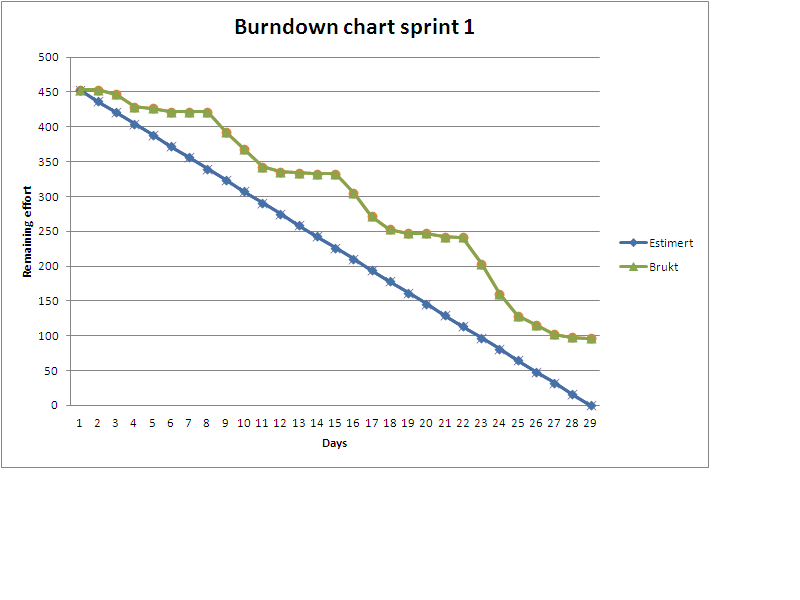
\includegraphics[width=\textwidth]{burndown1.png}
	\caption{Burndown chart sprint 1}
	\label{fig:burndown1}
\end{figure}

	\section{Customer feedback}

The customer was largely positive about our progress in Sprint 1. They were extremely pleased that we had managed to build a working prototype. They noted that we had gotten far in already being able to send and receive messages, and that boded well for our ability to implement some “interesting” components later in the process.
\newline
\newline
There was, however a number of points they felt needed work. They had a number of comments on the GUI; both the rudimentary version used in the demo and the mock up “paper” prototype that we had sent them earlier. They wanted lable (drill, exercise, etc) and the sent time/date included in the inbox display of emails, as well as security clearance. They also wanted security clearance visible in the top left corner whenever classified information was visible on the page. 
\newline
\newline
They also had a number of comments about our project planning and use of Scrum. Most importantly, we had fallen into the practice of using too general posts, leading ambiguities about what parts of that post was included in the current Sprint and what was to be implemented later. We agreed to avoid this in the future, and resolved to include this in our discussions of Sprint 2. There was also some minor comments on various sub-tasks and small ambiguities to clear up, but nothing major.

	\section{Conclusion}

Despite a number of setbacks, some late planning and technical problems, the first sprint was a success. We managed to create a working prototype, as well as a number of (as of yet) unconnected components. We hammered out a functional architecture, which should be more than robust enough to handle any changes forced on it in the next sprint. And we are well on schedule when it comes to the documentation; including a number of templates and designs for the type of files we produce a lot of (agendas and minutes especially). 

%\chapter{Sprint 2}

	\chapter{Sprint 2}

\section{Sprint 2 - Planning}
Finishing the first sprint left us with a working demo that could send and receive emails. After meeting with Thales and showing them the demo, we came to the conclusion that we needed to perform a thorough study regarding the security aspect of the application. The security issues that were most vital to the functionality of the application were local storage of program data and secure sending with \gls{ssl1} (fulfilling customer requirement 5.1). We also realized that we needed more concise documentation of the architecture, which was a bit vague at this point. This was something which we did intentionally, as we weren’t sure what we could implement and what would be left as a pre- and poststudy. 
\newline
\newline
We knew that the second sprint would be hectic. We did not have much room for extra workloads, as the regular documentation work takes a lot of time. Thales' request for a security prestudy did not make it easier, but we agreed to continue at a higher pace with both the frontend and backend part of the application. The \gls{gui} of the frontend was almost non existing, so it had to be developed from scratch within just one sprint. One of the biggest goals was to implement the ability to add attributes to outgoing messages, so that they could be prioritized on these attributes, as well as getting a \gls{gui} with a more complete look and feel.
\newline
\newline
Sprint two had a lot of time set aside for further documentation. This was crucial for being able to get better progress in the later sprints regarding programming. Most members of the project group were set to work on the documentation while two of the developers continued to work with the application. 

	\section{Sprint 2 - Concrete project work plan}

\textbf{Milestone:} Have a working demo to show the customer and advisor. In addition to the milestone of sprint 1, it should incorporate an inbox and outbox in a much more comprehensive way where all \gls{gui} functionality is complete. At completion of the sprint substantial documentation regarding architecture and security prestudy should also be completed.
\newline
\newline
See table \ref{tab:sprint2tasks} at page \pageref{tab:sprint2tasks}.
\newline
\newline
Explenations of the short names in the table:\\
KP-10: Meetings\\
KP-21: Browse previously sent messages\\
KP-76: Sending a message\\
KP-78: Browse inbox\\
KP-82: Read message\\
KP-89: Browse outbox\\
KP-90: Bottom menubar\\
KP-91: Security prestudy\\
KP-96: Architecture documentation\\

\begin{table}
\begin{tabularx}{\linewidth}{>{\setlength\hsize{.2\hsize}}X|>{\setlength\hsize{1.5\hsize}}X|>{\setlength\hsize{.1\hsize}}X}
\textbf{Main activity} &  \textbf{Sub-task} & \textbf{Estimate}\\ \hline \hline
KP-1 & Setup of Jira & 5h\\ \hline
KP-2 & Report work & 70h\\ \hline
KP-3 & Set up programming environment & 5h \\ \hline
KP-9 & Group administration & 25h\\ \hline
KP-10 & Meetings with Thales & 15h\\ \hline
KP-10 & Meetings with Mohnsen Anvaari & 6h\\ \hline
KP-10 & Internal meetings & 60h\\ \hline
KP-10 & Lectures & 8h\\ \hline
KP-21 & Show basic listing of all elements in list & 3h \\ \hline
KP-21 & Style elements of list & 8h \\ \hline
KP-60 & Meeting and document writing & 18h \\ \hline
KP-76 & Implement metadata structure and show it & 6h \\ \hline
KP-78 & Show basic listing of all elements in list & 3h \\ \hline
KP-78 & Style elements of list & 8h \\ \hline
KP-82 & Showing all metadata & 4h \\ \hline
KP-82 & Showing all message subject and text & 3h \\ \hline
KP-82 & Reply/Delete/Forward & 8h \\ \hline
KP-89 & Show basic listing of all elements of list & 3h \\ \hline
KP-89 & Style list for pretty viewing & 8h \\ \hline
KP-90 & Create bottom menu bar & 3h \\ \hline
KP-91 & Secure sending & 8h \\ \hline
KP-91 & Secure storage on phone & 10h \\ \hline
KP-91 & Signing and verification & 13h \\ \hline
KP-91 & Limitations and facilities of Android & 15h \\ \hline
KP-91 & Security requirements by CT & 13h \\ \hline
KP-96 & Fullfillment of requirements & 4h \\ \hline
KP-96 & Graphical view of architecture & 18h \\ \hline
KP-96 & Frontend & 5h \\ \hline
KP-96 & Backend & 5h \\ \hline
 &  & 360h
\end{tabularx}
\caption{Sprint 2 tasks} \label{tab:sprint2tasks}
\end{table}

	\section{Sprint 2 - Sprint duration}
The second sprint started with a planning session on September 18th and ended at October 7th. 

\section{Sprint 2 - Sprint goal}
The goal of the second sprint was to increase the depth of the documentation, especially the architecture documentation, and get further insight into the security issues that arise with several parts of the application. 
\newline
\newline
At the end of the sprint we were also going to show a demo to the Thales that would have the functionality of adding attributes to messages. 
\newline
\newline
In order to achieve this sprint’s goal, we needed one group member to document our architecture properly, two group members to continue the work with the application, while the rest of the group members looked into the security problems we were facing, and how we best could solve them.

	\section{Sprint 2 - Ordered sprint backlog}

\begin{itemize}
\item{}\textbf{Report work:} The report that is to be delivered at the end of the project needs a lot of work, and we have decided that we will use time on the report in every sprint.
\item{}\textbf{Group Administration:} To administrate on behalf of the entire group, to book group rooms and send emails to the customer, the advisor and the team to call in for meetings.
\item{}\textbf{Meetings:} Arranging meetings and the time we use on meetings.
\begin{itemize}
\item{}\textbf{Meetings with Thales:} We have weekly meetings with our customer so that we can get rapid feedback on what we do. To know if they agree with our decisions and that we haven't misunderstood the task thay have given us.
\item{}\textbf{Meetings with Mohnsen Anvaari:} We have regular meetings with our advisor so that he can give us feedback on how we are doing our work, and make sure that we do what are expected of us in the course.
\item{}\textbf{Internal meetings:} Every time we meet we first have a status meeting were we share what we have done and how far we have come with our tasks.
\item{}\textbf{Lectures:} There are some lectures during the semester, and we are adviced to paticipate in these. In this sprint there are 2 lectures and courses that we have decided to attend.
\end{itemize}

\newpage

\item{}\textbf{Browse previously sent messages:} make it possible to see all messages that have been previously sent, so that it is possible for the user to check that they actually were sent.
\begin{itemize}
\item{}\textbf{Show basic listing of all elements in list:} a basic listing of all elements should be implemented, and each data element in the list should have all necessary fields that are required.
\item{}\textbf{Style elements in list:} use design theory to make all the elements look presentable.
\end{itemize}
\item{}\textbf{Meeting and agenda document writing:} to write all the meetings agendas and minutes using the right template.
\item{}\textbf{Sending a message:} the user should be able to click the “New message” button, be brought to the new message page, create a message and send it pressing the “Send” button.
\begin{itemize}
\item{}\textbf{Implement metadata structure and show it:} implement all the fields that are required to send a message; from, to, classification, label, priority, and make them look presentable.
\end{itemize}
\item{}\textbf{Browse inbox:} the user should be able to show a list of all received messages, both read and unread.
\begin{itemize}
\item{}\textbf{Show basic listings of all messages received:} implement a basic list of all elements, and make sure that all necessary fields that are required are displayed.
\item{}\textbf{Style elements in list:} style each element of the list, so that it is pleasing to look at.
\end{itemize}
\item{}\textbf{Read message:} making the user able to read a message.
\begin{itemize}
\item{}\textbf{Showing all metadata:} implement all fields that are related to a message, and display them.
\item{}\textbf{Showing message subject and text:} show all fields that are related to a message; date received, from.
\item{}\textbf{Reply/Delete/Forward:} implement the buttons so that the user can reply to a message, delete a message and forward a message.
\end{itemize}
\item{}\textbf{Browse outbox:} the user should be able to show a list of all messages that are waiting to be sent, or haven’t been sent yet.
\begin{itemize}
\item{}\textbf{Show basic listing of all elements in list:} implement a basic listing of all elements, and that each data element in the list has all necessary fields that are required.
\item{}\textbf{Style list for pretty viewing:} make the list pleasing to look at.
\end{itemize}
\item{}\textbf{Bottom menu bar:} implement the bottom menu bar so that a user can switch between pages using the menu bar.
\begin{itemize}
\item{}\textbf{Create bottom menu bar:} implement the menu bar and make it presentable and useful by applying design theory.
\end{itemize}

\newpage

\item{}\textbf{Security Pre-study:} dig deeper into the security aspects of Android, in order to make well informed decisions.
\begin{itemize}
\item{}\textbf{Secure sending:} write security documentation on secure sending.
\item{}\textbf{Secure storage on phone:} write documentation regarding secure storage of data and password.
\item{}\textbf{Signing and verification:} finding out how secure signing works, and write documentation on it.
\item{}\textbf{Limitations and facilities of Android:} what are the limitations regarding Android security, and what does Android facilitate when it comes to encapsulation? Is data in memory secure? Find the answers to the questions and document it.
\item{}\textbf{Security requirements:} write a summary of the documentation linked to by Tellefsen.
\end{itemize}
\item{}\textbf{Architecture documentation:} make an architectural description document, so that we know that the code fulfills all the requirements.
\begin{itemize}
\item{}\textbf{Fulfillment of requirements:} describe how our architecture fulfills the security, usability and latency requirements.
\item{}\textbf{Graphical view of architecture:} create a graphical view of the architecture, both backend and frontend.
\item{}\textbf{Frontend:} document the frontend properly.
\item{}\textbf{Backend:} document the backend properly.
\end{itemize}
\end{itemize}


	\section{Sprint 2 - System design}
After the second sprint, the system worked in this way: A user opens the mail application on his phone. He is then brought directly to a tab called “Folders” which at first displays all the inbox messages of the application.
\newline
\newline
In the “Folders” tab, the user gets the opportunity to choose either “Inbox”, “Outbox” or “Sent” from a dropdown menu. “Inbox” shows a list of received messages, which the user can read one by one by clicking them. “Sent” takes the user to a list of sent messages which works in the same way as “Inbox”. “Outbox” is in this iteration not yet implemented. There is also a button that is called sort, which is also not implemented.The backend of this feature works in the same way as it did after the first sprint. 
\newline
\newline
If the user selects the “New Message” tab, he is taken to the message creation screen where he can add recipients and subject to the message. In this iteration we also included the functionality of adding attributes to the messages sent (Security Label, Message Priority and Message Type). The attributes are sent along with the message in the message header.
\newline
\newline
The changes to our application with respect to functionality in sprint one, is the addition of attributes to the messages and the menu bar at the top. It is all now packed into a better user experience where the number of errors a user can do is a lot fewer. 


	\section{Sprint effort}

See tabel \ref{tab:effortweekss2} at page \pageref{tab:effortweekss2}
\begin{table}
\begin{tabularx}{\linewidth}{>{\setlength\hsize{.625\hsize}}X|>{\setlength\hsize{0.3\hsize}}X|>{\setlength\hsize{0.5\hsize}}X|>{\setlength\hsize{0.5\hsize}}X|>{\setlength\hsize{0.5\hsize}}X|>{\setlength\hsize{.3\hsize}}X}
Group no: 15 Date: 17/0-07/10  \\ \hline
\textbf{Activity} & \textbf{Start} & \textbf{W5} 17/09-23/09 & \textbf{W6} 24/09-30/09 & \textbf{W7} 01/10-07/10 & \textbf{Activity sums} \\ \hline \hline
Management & \textbf{E:} A:0 & \textbf{E:/} A:5.5/5.5 & \textbf{E:/} A:2.5/8 & \textbf{E:/} A:1.5/9.5 & \textbf{E:35} A:9.5  \\ \hline
Lectures & \textbf{E:0} A:0 & \textbf{E:0/0} A:6/6 & \textbf{E:/} A:3.5/9.5 & \textbf{E:/} A:0/9.5 & \textbf{E:8 } A:9.5  \\ \hline
Planning & \textbf{E:0} A:0 & \textbf{E:0/0} A:38.5/38.5 & \textbf{E:} A:11.5/50 & \textbf{E:/} A:16.5/66.5 & \textbf{E:99 } A:66.5  \\ \hline
Pre study & \textbf{E:} A:0 & \textbf{E:0/0} A:10/10 & \textbf{E:0/0} A:10.5/20.5 & \textbf{E:/} A:8.5/29 & \textbf{E:59} A:29  \\ \hline
Requirement & \textbf{E:} A:0 & \textbf{E:/} A:/ & \textbf{E:/} A:/ & \textbf{E:/} A:/ & \textbf{E: } A:  \\ \hline
Design & \textbf{E:0} A:0 & \textbf{E:/} A:18.5/18.5 & \textbf{E:/} A:40/58.5 & \textbf{E:/} A:42/100.5 & \textbf{E:57} A:100.5  \\ \hline
Implementation & \textbf{E:0} A:0 & \textbf{E:0/0} A:0/0 & \textbf{E:/} A:/ & \textbf{E:/} A:/ & \textbf{E: } A:  \\ \hline
Documentation & \textbf{E:0} A:0 & \textbf{E:0/0} A:40/40 & \textbf{E:/} A:59.5/99.5 & \textbf{E:/} A:55.5/155 & \textbf{E:102 } A:155  \\ \hline
Evaluation & \textbf{E:0} A:0 & \textbf{E:0/0} A:0/0 & \textbf{E:0/0} A:0/0 & \textbf{E:0/0} A:0/0 & \textbf{E:0 } A:0  \\ \hline
Demonstration & \textbf{E:0} A:0 & \textbf{E:0/0} A:0/0 & \textbf{E:0/0} A:0/0 & \textbf{E:0/0} A:0/0 & \textbf{E:0 } A:0  \\ \hline
Period sums & E:0 \textbf{A:0} & E:0/0 \textbf{A:118.5/118.5} & E:/ \textbf{A:127.5/246} & E:/ \textbf{A:124/370} & E:360 \textbf{A:370}
\end{tabularx}

\textbf{Period coomments:}


\textbf{Activity comments:}

\caption{Table for effort registrations in sprint 2} \label{tab:effortweekss2}
\end{table}

	\begin{figure}
	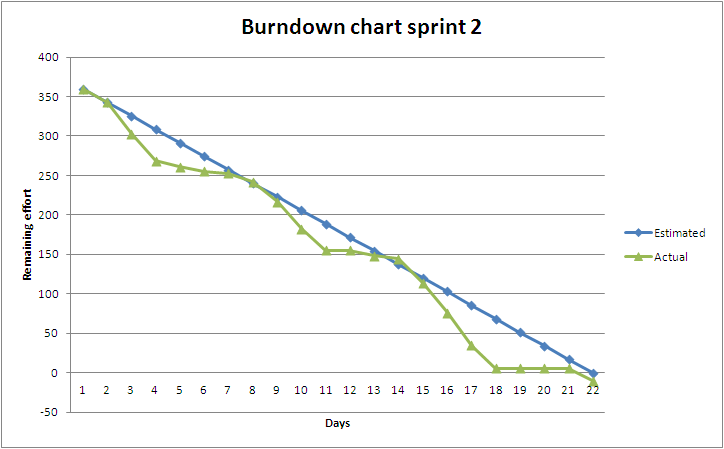
\includegraphics[width=\textwidth]{burndown2.png}
	\caption{Burndown chart sprint 2}
	\label{fig:burndown2}
\end{figure}

	\section{Customer feedback}

	\section{Sprint 2 - Conclusion}
The second sprint was well planned and with tasks that was doable in the given time-span we had available. We ended up with a lot more thorough documentation, especially on the parts regarding security and system architecture. We also ended up with a new demo with additional functionality of adding attributes to the messages. During this sprint there was also less time wasted on group bureaucracy since routines and group dynamics had become more integrated in the daily routines. We managed to complete all the goals we set for this sprint and can therefore conclude that the sprint was a success.     

\chapter{Sprint 3}

	\section{Sprint 3 - Concrete project work plan}

\textbf{Milestone:} Have a working demo to show the customer and adviser. In addition to the milestone of sprint 2, it should incorporate better and more responsive user interface, the possibility of sending messages with and without attachments through the XOmail SMTP-gateway and the possibility to sign and verify messages using S/MIME. In addition a data usage study should be be added to the documentation describing the applications data usage and ways to reduce these.

See table \ref{tab:sprint3tasks} at page \pageref{tab:sprint3tasks}.
\begin{table}
KP-10: Meetings\\
KP-19: Log in to App\\
KP-26: Iteration network service\\
KP-28: Sending message with attachments\\
KP-29: Answer and forward message\\
KP-32: Add signing to messages\\
KP-34: Settings menu\\
KP-79: Receiving message with attachment\\
KP-109: Wireshark study\\
KP-119: Instant message\\
KP-127: Delete message\\
KP-131: GUI-Issues\\

\begin{tabularx}{\linewidth}{>{\setlength\hsize{.2\hsize}}X|>{\setlength\hsize{1.5\hsize}}X|>{\setlength\hsize{.1\hsize}}X}
\textbf{Main activity} &  \textbf{Sub-task} & \textbf{Estimate}\\ \hline \hline
KP-2 & Report work & 68h\\ \hline
KP-9 & Group administration & 2h\\ \hline
KP-10 & Meetings with Thales & 18h\\ \hline
KP-10 & Meetings with Mohnsen Anvaari & 15h\\ \hline
KP-10 & Internal meetings & 60h\\ \hline
KP-10 & Lectures & 15h\\ \hline
KP-19	& Create basic GUI & 1h\\ \hline
KP-19	& Find solution for encrypting the login information & 1h\\ \hline
KP-19	& Persist and fetch login data & 5h\\ \hline
KP-26 & Implement threaded SMTP queue & 15h\\ \hline
KP-26 & Implement stripping of message based on network connection & 8h\\ \hline
KP-26	& Implement usage IMAP specific attributes & 6h\\ \hline
KP-26 & Save messages downloaded from server & 4h\\ \hline
KP-26 & Update message IMAP message status & 6h\\ \hline
KP-26 & Implement pull strategy & 6h\\ \hline
KP-26 & Implement push strategy & 10h\\ \hline
KP-26 & Implement handling for pre-send processing of messages & 8h\\ \hline
KP-26 & Implement handling for control-messages & 8h\\ \hline
KP-28	& Study & 2h\\ \hline
KP-28	& Find what attachments we should support & 1h\\ \hline
KP-28	& Documentation of choice for attachments & 1h\\ \hline
KP-28 & Implement & 6h\\ \hline
KP-28 & Implement GUI & 8h\\ \hline
KP-29	& Locking security label on reply and forward & 1h\\ \hline
KP-32	& Implement a keystore for saving and loading trusted keys & 8h\\ \hline
KP-32 & SPIKE: bouncycastle for android & 4h\\ \hline
KP-32 & Implement S/MIME signing of messages & 10h\\ \hline
KP-32 & Implement verification of signing messages & 10h\\ \hline
KP-34	& Set update interval for checking of mail to avoid pulling & 1h\\ \hline
KP-34	& Set security labels available & 1h\\ \hline
KP-34	& Standard receiver of instant message & 1h\\ \hline
KP-35	& Compression study & 6h\\ \hline
KP-79	& Study & 2h\\ \hline
KP-79	& Implement & 6h\\ \hline
KP-79	& Document & 2h\\ \hline
KP-109 & Learn Wireshark & 4h\\ \hline
KP-109 & Document Wireshark & 2h\\ \hline
KP-109 & Analyse traffic & 10h\\ \hline
KP-109 & Discussion & 3h\\ \hline
KP-119 & Find design solution & 1h\\ \hline
KP-119 & Incorporate instant message button into GUI & 1h\\ \hline
KP-119 & Create send instant message view & 2h\\ \hline
KP-127 & Delete from local strage & 2h\\ \hline
KP-127 & Delete from mail server & 4h\\ \hline
KP-127 & Update GUI & 2h\\ \hline
KP-131 & Menu & 1h\\ \hline
KP-131 & Header & 1h\\ \hline
KP-131 & Change security labels to upper case & 1h\\ \hline
 &  & 360h
\end{tabularx}
\caption{Sprint 3 tasks} \label{tab:sprint3tasks}
\end{table}

	

\section{Sprint 3 - Ordered sprint backlog}

\begin{itemize}
\item{}\textbf{Report work:} the report that is to be delivered at the end of the project needs a lot of work, and we have decided that we will use time on the report in every sprint.
\item{}\textbf{Group Administration:}to administrate on behalf of the entire group, to book group rooms and send emails to the customer, the advisor and the team to call in for meetings.
\item{}\textbf{Meetings:}arranging meetings and the time we use on meetings.
\begin{itemize}
\item{}\textbf{Meetings with Thales:} we have weekly meetings with our customer so that we can get rapid feedback on what we do. To know if they agree with our decisions and that we haven't misunderstood the task thay have given us.
\item{}\textbf{Meetings with Mohnsen Anvaari:} we have regular meetings with our advisor so that he can give us feedback on how we are doing our work, and make sure that we do what are expected of us in the course.
\item{}\textbf{Internal meetings:} we have almost daily meetings to learn what everybody has been doing lately, and how far we have come in our tasks; what is left and what is done.
\item{}\textbf{Lectures:} there are some lectures during the semester, and we are adviced to paticipate in these. In this sprint there are 2 lectures and courses that we have decided to attend.
\end{itemize}
\item{}\textbf{Log in to app:}as a user I should be able to log in via the login screen so that I after this process am an authorized user inside the program.
\begin{itemize}
\item{}\textbf{Create basic GUI:} create a basic GUI for login. This means a GUI that has a username and password field, and a "Log in" button
\item{}\textbf{Find solution for encrypting the login information:} figure out what solution we are going to use for save the login information. This means that we need to decide for an implementation based on Magnus' documentation. The best is if we can make a solution that is so good that we don’t need to revise it.
\item{}\textbf{Persist and fetch login data:} implement the saving and fetching of the login data, making the login functionality complete.
\end{itemize}
\item{}\textbf{Iteration network service:} as a programmer I should extend the communication implementation to support more features, so that we can have message priorities, message types, message classification, message status and notification of failed deliveries.
\begin{itemize}
\item{}\textbf{Implement threaded SMTP queue:} Implement all SMTP related method to run in a separate thread other then the gui-thread, in order to ensure responsive user interface.
\item{}\textbf{Implement stripping of message based on network connection:} Implement a pre-sending processing step for XOMessage which removes possible attachment based on the network connection at the current time. This should be done through the use of interfaces to ensure modifiability. 
\item{}\textbf{Implement usage IMAP specific attributes:} Implement the usage of IMAP states into NetworkService so that the phone and server is in a consistent state. E.g SEEN flag ect. 
\item{}\textbf{Save messages downloaded from server:} Persist a number of the latest received messages locally on the device. The number of messages that are to be persisted should be determined by an option in the settings menu.
\item{}\textbf{Update message IMAP message status:} Update flags on messages whenever the state changes, e.g. the messages is opened locally on the device and this change should be reflected on the server as well.
\item{}\textbf{Implement pull strategy:} Implement a pull strategy for periodically pulling the mail server for new messages.
\item{}\textbf{Implement push strategy:} Implement a push strategy using the IMAP-Idle command in order to get the server to push messages to the device. 
\item{}\textbf{Implement handling for pre-send processing of messages:} Implement a pre-send processing of messages that handles template codes. e.g. \#GPS : will fetch the gps data and inject them into the message before sending. 
\item{}\textbf{Implement handling for control-messages:} Implement a onReceive handler the stops control-messages of getting through to the user, and in addition responds to the control-message in the correct way.
\end{itemize}
\item{}\textbf{Sending message with attachments:} the user should be able to send a message containing different attachments.
\begin{itemize}
\item{}\textbf{Study:} figure out how to fetch images, i.e. from the phone, or another app on the phone. How does it work on android?
\item{}\textbf{Find what attachments we should support:} based on how difficult it is to get images, GPS coordinates etc, make a decision on what kind of attachments we should support. Maybe there are some things we should be careful about using, maybe it isn't. Find out!
\item{}\textbf{Documentation of choice for attachments:} make documentation about why we chose the attachments we chose.
\item{}\textbf{Implement:} Imlement sending attachments based on what found out in the study. What this tasks means, depends on which attachments we are to send. A picture will be sent differently than GPS coordinates. Maybe the coordinates should be implemented into the message body, whilst the image will be shown by a button. All this should be reveiled during the Study of this main task. 
\item{}\textbf{Implement GUI:} Implement the gui-side of sending messages with attachments based on the conclusion of the study. How to send gps vs binary data.
\end{itemize}
\item{}\textbf{Answer and forward a message:} as a user I want to be able to utilize the "Reply" and "Forward" buttons that is associated with each message so that I am brought to the correct screen for each of these operations.
\begin{itemize}
\item{}\textbf{Locking security label on reply and forward:} the user should not be able to set the security label of a message when he/she replies or forwards.
\end{itemize}
\item{}\textbf{Add signing to messages:} as a programmer I should be able to create or use an existing library for digital signing of messages, so that only signed messages are identified by the recipient as a valid message.
\begin{itemize}
\item{}\textbf{Implement a keystore for saving and loading trusted keys:} Implement a way of safely storing keys and key derivatives locally on the device. 
\item{}\textbf{SPIKE: bouncycastle for android :} Research the use of bouncycastle on an android device in order to find out if this is a possible solution for encryption, signing and verification of messages.
\item{}\textbf{Implement S/MIME signing of messages:} Bases on the bouncycastle spike, implement the signing of messages. 
\item{}\textbf{Implement verification of signing messages:} Based on the bouncycastle spike, implement the verification of signing messages.
\end{itemize}

\newpage

\item{}\textbf{Settings menu:} as a user, I should be able to utilize the settings menu to alter different settings of the app, so that the settings are set to what I prefer.
\begin{itemize}
\item{}\textbf{Set update interval for checking of messages to avoid pulling:} this is a setting making it possible for the user to choose to have push or pull solution for messages. If they chose to use push, the app always have a connection up to the server. If the user don’t have an Internet connection, the app will try to set up the connection all the time and use a lot of battery. If the user chose pull, the app uses a predefined interval for how often the app should check for messages. So one solution could be a radio button list: "Push", "Pull".
\item{}\textbf{Set security labels available:} the user should be able to choose which Security Labels he will find available in the dropdown when sending a new message.
\item{}\textbf{Standard receiver of instant message:} the user should be able to set a standard receiver to use when sending an instant message.
\end{itemize}
\item{}\textbf{Compression study:} as a programmer I want to be able to create or find a library that minimize data traffic that is needed to send a message, so that the messages are sent faster over low speed Internet connections.
\item{}\textbf{Receiving message with attachment:} as a user I should be able to receive a message with an attachment and to see the attachment.
\begin{itemize}
\item{}\textbf{Study:} how should we show the different attachments? Use some embedded features of android or use our own? Are the attachments shown immediately or do we click a button to show it? Do some studies so that you are able to answer all the questions above.
\item{}\textbf{Implement:} implement showing attachments based on what was found out in the study. What this task involves, depends on which attachments we receive. A picture will be shown differently than GPS coordinates. Maybe the coordinates should be implemented into the message body, while the image will be shown by a button, as figured in the above study task.
\item{}\textbf{Document:} document the different options that are found relevant for the solution of the task, but was excluded due to complexity or because it was a bad alternative.
\end{itemize}
\item{}\textbf{Wireshark study:} do a study on wireshark and network traffic of our app.
\begin{itemize}
\item{}\textbf{Learn Wireshark:} figure out how Wireshark works, and learn to use it.
\item{}\textbf{Document Wireshark:} an important part of the Wireshark study is to document how Wireshark works, the reason behind using Wireshark in this project and what results we get from it. Create statistics on the gathered results.
\item{}\textbf{Analyse traffic:} find out how the data from all the traffic from our app should be analyzed. How much is regular package data that always will flow when sending a message, how much of it is the content, and how much is data that we don’t need to send, e.g. what data is unnecessary polling, if any?
\item{}\textbf{Discussion:} do a discussion on the findings of the data gathering. We will not be able to do a conclusion yet, as we have not implemented sending of messages with pictures, videos etc. Document your thoughts.
\end{itemize}
\item{}\textbf{Instant message:} the user should be able to send an instant message using only three touches.
\begin{itemize}
\item{}\textbf{Find design solution:} find out how to implement the instant message feature. Where should the instant message button be placed? What is the fastest solution? How should the send instant message window look like?
\item{}\textbf{Incorporate instant message button into GUI:} get a working button in the GUI that takes the user to the instant message view.
\item{}\textbf{Create send instant message view:} create a view that is to be used for sending an instant message, based on what is found to be the best design solution.
\end{itemize}
\item{}\textbf{Delete message:} the user should be able to delete a message that is received.
\begin{itemize}
\item{}\textbf{Delete from local storage:} Implement the response of deleting a message locally whenever a user wants to delete the message.
\item{}\textbf{Delete from mail server:} Implement the response of deleting a message from the mail server whenever a user wants to delete the message.
\item{}\textbf{Update GUI:} Implement the response of removing a message from the gui whenever a delete operation is completed. 
\end{itemize}
\item{}\textbf{GUI-Issues:} revisions of the GUI based on input from Thales.
\begin{itemize}
\item{}\textbf{Menu:} the top menu bar must be made smaller by removing the text, and only use pictures.
\item{}\textbf{Header:} remove the header saying XO-mail. It is not necessary.
\item{}\textbf{Change security labels to upper case:} all the security labels should be of the format CAPS\_LOCK! Upper case and underscore for spaces.
\end{itemize}
\end{itemize}



	\section{Sprint 3 - Effort}

See table \ref{tab:effortweekss3} at page \pageref{tab:effortweekss3}

\newpage

\begin{table}[htb]
\begin{tabularx}{\linewidth}{>{\setlength\hsize{.625\hsize}}X|>{\setlength\hsize{0.3\hsize}}X|>{\setlength\hsize{0.5\hsize}}X|>{\setlength\hsize{0.5\hsize}}X|>{\setlength\hsize{0.5\hsize}}X|>{\setlength\hsize{.3\hsize}}X}
Group no: 15 Date: 8/10-28/10  \\ \hline
\textbf{Activity} & \textbf{Start} & \textbf{W8} 8/10-14/10 & \textbf{W9} 15/10-21/10 & \textbf{W10} 22/10-28/10 & \textbf{Activity sums} \\ \hline \hline
Management & \textbf{E:0} A:0 & \textbf{E:0/0} A:9.5/9.5 & \textbf{E:2/2} A:2/11.5 & \textbf{E:0/2} A:0/11.5 & \textbf{E:2} A:11.5  \\ \hline
Lectures & \textbf{E:0} A:0 & \textbf{E:0/0} A:0/0 & \textbf{E:0/0} A:0/0 & \textbf{E:15/15} A:6/6 & \textbf{E:15} A:6  \\ \hline
Planning & \textbf{E:34} A:0 & \textbf{E:34/34} A:31.5/31.5 & \textbf{E:34/68} A:10.5/42 & \textbf{E:25/93} A:16.5/58.5 & \textbf{E:93} A:58.5  \\ \hline
Pre study & \textbf{E:2} A:0 & \textbf{E:2/2} A:1.5/1.5 & \textbf{E:12/14} A:18/19.5 & \textbf{E:2/16} A:2/21.5 & \textbf{E:16} A:21.5  \\ \hline
Requirement & \textbf{E:0} A:0 & \textbf{E:0/0} A:0/0 & \textbf{E:0/0} A:0/0 & \textbf{E:0/0} A:0/0 & \textbf{E:0} A:0 \\ \hline
Design & \textbf{E:7} A:0 & \textbf{E:7/7} A:15.5/15.5 & \textbf{E:7/14} A:40.5/56 & \textbf{E:7/21} A:46/102 & \textbf{E:21} A:102  \\ \hline
Implementation & \textbf{E:37} A:0 & \textbf{E:37/37} A:23/23 & \textbf{E:57/94} A:36.5/59.5 & \textbf{E:33/127} A:30.5/90 & \textbf{E:127} A:90  \\ \hline
Documentation & \textbf{E:40} A:0 & \textbf{E:40/40} A:75/75 & \textbf{E:8/48} A:8/83 & \textbf{E:38/86} A:39.5/122.5 & \textbf{E:86} A:122.5  \\ \hline
Evaluation & \textbf{E:0} A:0 & \textbf{E:0/0} A:0/0 & \textbf{E:0/0} A:0/0 & \textbf{E:0/0} A:0/0 & \textbf{E:0 } A:0  \\ \hline
Demonstration & \textbf{E:0} A:0 & \textbf{E:0/0} A:0/0 & \textbf{E:0/0} A:0/0 & \textbf{E:0/0} A:0/0 & \textbf{E:0 } A:0  \\ \hline
Period sums & E:120 \textbf{A:0} & E:120/120 \textbf{A:156/156} & E:120/240 \textbf{A:115.5/271.5} & E:120/360 \textbf{A:140.5/412} & E:360 \textbf{A:412} \\ \hline
\end{tabularx}

\caption{Table for effort registrations in sprint 3} \label{tab:effortweekss3}
\end{table}

\textbf{Period comments:}
\begin{itemize}
\item{}\textbf{W8:}
\begin{itemize}
\item{}\textbf{Management:} We forgot to estimate some of the weekly work that had to be done, so therfore there were used some more effort then planned.
\item{}\textbf{Documentation:} Some of the group members had a lot to do in another class, so they postponed some of the documentation tasks for later.
\end{itemize}
\item{}\textbf{W9:}
\begin{itemize}
\item{}\textbf{Pre study:}Some of the topics that we were studying this week was a lot harder to learn than expected.
\end{itemize}
\item{}\textbf{W10:}
\begin{itemize}
\item{}\textbf{Lectures:}The lecture was a bit shorter than announced, and not all group members participated.
\end{itemize}
\end{itemize}

\newpage

\textbf{Activity comments:}
\begin{itemize}
\item{}\textbf{Planning:} The sprint planning did not take as much time as in the other sprints. This time we agreed on the tasks in shorter amout of time.
\item{}\textbf{Design:} It was some more design work than we thought, and a lot of the tasks that we thought was implementation turned out to be design instead.
\item{}\textbf{Implementation:} Some of the implementation tasked turned out to be design tasks instead.
\end{itemize}

\chapter{Sprint 4}

\chapter{Changelog}

\part{Conclusion \& Reflection}

\chapter{Reflection}

\glossary{name={Stanag 4406}, description={The NATO standard for Military Messaging based on X.400}}
\glossary{name={SMTP}, description={"Simple Mail Tranfer Protocol" defined by RFC 5321}}

\printglossary

\begin{thebibliography}{99}
\bibitem{bib:xomail} XOmail. Retrieved 2012-09-12 from <http://www.xomail.com>
\bibitem{bib:stanag} Stanag 4406. Retrieved 2012-09-12 from <http://www.isode.com/solutions/military-messaging.html>
\bibitem{bib:smtp} Simple Mail Transfer Protocol. Retrieved 2012-09-12 from <http://en.wikipedia.org/wiki/Smtp>
\bibitem{bib:imap} Internet Message Access Protocol. Retrieved 2012-09-12 from <http://en.wikipedia.org/wiki/Imap>
\bibitem{bib:thales} Thales Norway AS. Retrieved 2012-08-28 from <http://www.thales.no/pub/sites/index.php?siteID=4\&m=1>
\bibitem{bib:git} Git \& GitHub. Retrieved 2012-09-10 from <https://github.com/>
\bibitem{bib:android} http://developer.android.com/design/get-started/principles.html
\bibitem{bib:pandroid} http://developer.android.com/design/patterns/pure-android.html
\bibitem{bib:pke} Public Key Encryption. Retrieved 2012-09-18 from <http://en.wikipedia.org/wiki/Public\_key>
\bibitem{bib:ds} Digital signing. Retrieved 2012-09-18 from <http://en.wikipedia.org/wiki/Digital\_signature>
\bibitem{bib:smime} S/MIME. Retrieved 2012-09-18 from <http://en.wikipedia.org/wiki/S/MIME>
\bibitem{bib:gmail} Gmail and S/Mime. Retrieved 2012-09-23 from <http://www.scientificcomputing.com/is-your-e-mail-secure.aspx>
\bibitem{bib:r2mail2} R2Mail2. Retrieved 2012-09-23 from <https://play.google.com/store/apps/details?id=at.rundquadrat.android.r2mail2\&hl=no>
\bibitem{bib:waterfall} Waterfall Model. Retrieved 2012-09-23 from <en.wikipedia.org/wiki/Waterfall\_model>
\bibitem{bib:agile} Agile Development. Retrieved 2012-10-13 from <http://en.wikipedia.org/wiki/Agile\_development>
\bibitem{bib:kanban} Kanban. Retrieved 2012-10-13 from <http://en.wikipedia.org/wiki/Kanban\_(development)>
\bibitem{bib:asdas} Agile Software Development And Scrum. Retrieved 2012-09-10 from <http://www.mountaingoatsoftware.com/topics/scrum>
\bibitem{bib:scrum} Scrum (Development). Retrieved 2012-09-10 from <en.wikipedia.org/wiki/Scrum\_(development)>
\bibitem{bib:java} Java (Programming Language). Retrieved 2012-09-10 from
<http://en.wikipedia.org/wiki/Java\_programming\_language>
\bibitem{bib:andk} Android Native Development Kit (NDK). Retrieved 2012-09-10 from <http://developer.android.com/tools/sdk/ndk/index.html>
\bibitem{bib:slfa} Scripting Layer for Android (SL4A). Retrieved 2012-09-10 from <http://code.google.com/p/android-scripting/>
\bibitem{bib:php} PHP for Android (PFA). Retrieved 2012-09-10 from <http://phpforandroid.net/manual/en/index/faq>
\bibitem{bib:mbx} Monodroid by Xamarin. Retrieved 2012-09-10 from <http://xamarin.com/monoforandroid>
\bibitem{bib:xml} Extensible Markup Language (XML). Retrieved 2012-09-10 from <http://en.wikipedia.org/wiki/Xml>
\bibitem{bib:json} JavaScript Object Notation (JSON). Retrieved 2012-09-10 from <http://www.json.org/xml.html>
\bibitem{bib:xstream} Xstream. Retrieved 2012-10-27 from http://xstream.codehaus.org/
\bibitem{bib:ibm} Xstream. Retrieved 2012-10-27 from http://www.ibm.com/developerworks/java/library/x-xstream/index.html
\bibitem{bib:kolawa} Kolawa, Adam; Huizinga, Dorota (2007). Automated Defect Prevention: Best Practices in Software Management. Wiley-IEEE Computer Society Press. p. 426. ISBN 0-470-04212-5
\bibitem{bib:junit} Junit. Retrieved 2012-10-01 from http://en.wikipedia.org/wiki/JUnit
\bibitem{bib:mock} Mock objects. Retrieved 2012-10-01 from http://en.wikipedia.org/wiki/Mock\_object
\bibitem{bib:mockito} "Features and Motivations". Retrieved 2010-12-29
\bibitem{bib:mocks} Fowler, Martin (2007). "Mocks Aren't Stubs". Retrieved 2010-12-29.
\bibitem{bib:greenmail} Greenmail. Retrieved 2012-10-01 from http://www.icegreen.com/greenmail/
\bibitem{bib:latex} LaTeX. Retrieved 2012-09-25 from http://www.latex-project.org/intro.html
\bibitem{bib:atlassian} Jira overview. Retrieved 2012-09-25 from http://www.atlassian.com/software/jira/overview
\bibitem{bib:jira} Jira. Retrieved 2012-09-25 from http://en.wikipedia.org/wiki/JIRA
\bibitem{bib:green} Grennhopper. Retrieved 2012-09-25 from http://www.atlassian.com/software/greenhopper/overview
\bibitem{bib:netbeans} NetBeans. Retrieved 2012-09-25 from http://netbeans.org/features/index.html
\bibitem{bib:ide} NetBeans IDE. Retrieved 2012-09-25 from http://en.wikipedia.org/wiki/NetBeans\#NetBeans\_IDE
\bibitem{bib:service} Service. Retrieved 2012-09-08 from http://developer.android.com/reference/android/app/Service.html
\bibitem{bib:aidl} AIDL. Retrieved 2012-09-08 from http://developer.android.com/guide/components/aidl.html
\bibitem{bib:ibinder} IBinder. Retrieved 2012-09-08 from http://developer.android.com/reference/android/os/IBinder.html
\bibitem{bib:techtarget} Techtarget. Retrieved 2012-09-25 from http://searchsecurity.techtarget.com/definition/link-encryption
\bibitem{bib:ispec} IPSec. Retrieved 2012-09-25 from http://stackoverflow.com/questions/3960802/implementing-ipsec-protocol-in-java
\bibitem{bib:ssl} TLS. Retrieved 2012-09-25 from http://en.wikipedia.org/wiki/Secure\_Sockets\_Layer
\bibitem{bib:nli} NetBeans license. Retrieved 2012-10-08 from http://netbeans.org/about/legal/product-licences.html
\bibitem{bib:ali} Android license. Retrieved 2012-10-08 from http://developer.android.com/license.html
\bibitem{bib:amli} Andoid-maven-plugin. Retrieved 2012-10-08 from http://code.google.com/p/maven-android-plugin/
\bibitem{bib:mli} Maven license. Retrieved 2012-10-08 from http://maven.apache.org/license.html
\bibitem{bib:jli} Junit license. Retrieved 2012-10-08 from http://www.junit.org/license
\bibitem{bib:gli} GreenMail license. Retrieved 2012-10-08 from http://www.icegreen.com/greenmail/
\bibitem{bib:jmli} JavaMail-android. Retrieved 2012-10-08 from http://code.google.com/p/javamail-android/
\bibitem{bib:xli} Xstream license. Retrieved 2012-10-08 from http://xstream.codehaus.org/license.html
\bibitem{bib:bcli} BouncyCastle license. Retrieved 2012-10-08 from http://www.bouncycastle.org/licence.html
\bibitem{bib:lli} MiKTeX license. Retrieved 2012-10-08 from http://miktex.org/copying
\bibitem{bib:gili} Git license. Retrieved 2012-10-08 from http://git-scm.com/about/free-and-open-source
\bibitem{bib:cli} Cygwin license. Retrieved 2012-10-08 from http://cygwin.com/licensing.html
\bibitem{bib:apli} Apache 2.0 license. Retrieved 2012-10-08 from http://www.apache.org/licenses/LICENSE-2.0
\bibitem{bib:gpl1} GPL-1.0 license. Retrieved 2012-10-08 from http://www.gnu.org/licenses/gpl-1.0.html
\bibitem{gpl2} GPL-2.0 license. Retrieved 2012-10-08 from http://www.gnu.org/licenses/old-licenses/gpl-2.0.html
\bibitem{bib:gplw} GPL-2.0 w/Classpath Exception license. Retrieved 2012-10-08 from http://openjdk.java.net/legal/gplv2+ce.html
\bibitem{bib:mit} MIT X11 license. Retrieved 2012-10-08 from http://opensource.org/licenses/mit-license.php
\bibitem{bib:cddl} CDDL-1.0 license. Retrieved 2012-10-08 from http://opensource.org/licenses/cddl-1.0
\bibitem{bib:cpl} CPL-1.0 license. Retrieved 2012-10-08 from http://www.junit.org/license
\bibitem{bib:bsd} BSD license. Retrieved 2012-10-08 from http://en.wikipedia.org/wiki/BSD\_licenses
\bibitem{bib:ieee} IEEE829. Retrieved  2012-09-30 from http://gerrardconsulting.com/tkb/guidelines/ieee829/main.html
\bibitem{bib:vm} Kruchten, Philippe (1995, November). Architectural Blueprints — The “4+1” View Model of Software Architecture. IEEE Software 12 (6), pp. 42-50.
\bibitem{bib:crypto} Android crypto implementation. Retrieved 2012-10-07 from http://source.android.com/tech/encryption/android\_crypto\_implementation.html
\bibitem{bib:tech} Security. Retrieved 2012-10-07 from http://source.android.com/tech/security/index.html
\bibitem{bib:aas} Android activity states. Retrieved 2012-10-13 from http://developer.android.com/reference/android/app/Activity.html
\bibitem{bib:alc} Activity life cycle. Retrieved 2012-10-13 from http://developer.android.com/guide/components/activities.html
\bibitem{bib:aman} Android manifest. Retrieved 2012-10-13 from http://developer.android.com/guide/topics/manifest/manifest-intro.html
\bibitem{bib:imap} IMAP. Retrieved 2012-10-07 from http://www.isode.com/whitepapers/imap-idle.html
\end{thebibliography}

\part{Appendices}

	\appendix
	
	\chapter{Templates \& Standards}

\section{Agendas}

\subsection{Agenda for Advisor Meeting \#X}

\begin{tabular}{>{\bfseries}l l}	
Project name&Formal and secure messaging on a mobile platform\\
Calling by&Group 15\\
Time and date&2012-MM-DD HH:MI\\
Place&ITV-464\\
Attendees&Mohsen Anvaari from IDI\\
 & Aleksander, Ida, Kristin, Lars, Magnus og Nicklas from Group 15\\
Referent&Kristin from Group 15\\
\end{tabular}

\begin{enumerate}
\item{}\textbf{Approval of agenda}
\item{}\textbf{Approval of minutes of meeting from last advisor meeting}
\item{}\textbf{Comments to the minutes from last customer meeting}
\item{}\textbf{Approval of the status report}
\begin{enumerate}
\item{}\textbf{Summary}
\item{}\textbf{Work done in this period}
Status of the documents that are being created\\*
Meetings\\*
Other activities
\item{}\textbf{Problems}
What is interfering with the progress or taking resources? Problems are often risks that have taken effect.
\item{}\textbf{Planning of work for the next period}
Meetings\\*
Activities
\item{}\textbf{Other}
\end{enumerate}
\item{}\textbf{Review/approval of attached phase documents}
\item{}\textbf{Other issues}
\item{}\textbf{Next meeting}
\end{enumerate}

	
	\begin{figure}[htb]

\includepdf[pages=-]{YYYY-MM-DD-Agenda-Customer.pdf}

\end{figure}

	
	\begin{figure}[htb]

\includepdf[pages=-]{YYYY-MM-DD-Agenda-Internal.pdf}

\end{figure}

	
	\documentclass[a4paper,12pt]{article}
\usepackage{array}
\begin{document}
\title{Weekly Status Report \#X}
\maketitle
\begin{tabular}{>{\bfseries}l l}	
Project name&Formal and secure messaging on a mobile platform\\
Written by&Group 15\\
Week&Week WW\\
Dates&2012-MM-DD - 2012-MM-DD\\
Referent&Kristin from Group 15\\
\end{tabular}

\section{Activities done this week}
\section{Activities planned next week}
\section{Challenges ahead}
\section{Status summary}
\section{Milestones}
\begin{tabular}{l l l l}	
Name&Planned&Real&Result
\end{tabular}
\end{document}

	
	\documentclass[a4paper,12pt]{article}
\usepackage{array}
\begin{document}
\title{Minutes of meeting for advisor meeting \#X}
\maketitle
\begin{tabular}{>{\bfseries}l l}	
Project name&Formal and secure messaging on a mobile platform\\
Calling by&Group 15\\
Time and date&2012-MM-DD HH:MI\\
Place&ITV-464\\
Attendees&Mohsen Anvaari from IDI\\
 & Aleksander, Ida, Kristin, Lars, Magnus og Nicklas from Group 15\\
Referent&Kristin from Group 15\\
\end{tabular}
\section{Agenda approved}
\section{Minutes of meeting from last advisor meeting approved}
\section{Comments to the minutes from last customer meeting}
\section{Approval of the status report}
\subsection{Summary}
\subsection{Work done in this period}
Status of the documents that are being created\\*
Meetings\\*
Other activities\\*
\subsection{Problems}
What is interfering with the progress or taking resources? Problems are often risks that have taken effect.
\subsection{Planning of work for the next period}
Meetings\\*
Activities
\subsection{Other}
\section{Review/approval of attached phase documents}
\section{Other issues}
\section{Next meeting}
\end{document}

	
	\begin{figure}[htb]

\includepdf[pages=1]{YYYY-MM-DD-Minutes-Customer.pdf}

\end{figure}

\newpage

\begin{figure}[htb]

\includepdf[pages=2]{YYYY-MM-DD-Minutes-Customer.pdf}

\end{figure}

	
	
\title{Minutes of Meeting for Internal Meeting \#X}
\maketitle
\begin{tabular}{>{\bfseries}l l}	
Project name&Formal and secure messaging on a mobile platform\\
Calling by&Group 15\\
Time and date&2012-MM-DD HH:MI\\
Place&?\\
Attendees&Aleksander, Ida, Kristin, Lars, Magnus and Nicklas from Group 15\\
Referent&Kristin from Group 15\\
\end{tabular}

\section{Agenda approved}
\section{Minutes of meeting from last internal, customer and advisor meeting approved}
\section{Case name}
\subsection{Sub item}
\subsection{Sub item}
\section{Other issues}
\section{Next meeting}


	\chapter{Agendas}

\section{Advisor}
The following pages include all agendas for advisor meetings.
\newpage
\begin{figure}[htb]
\includepdf[pages=1]{2012-09-04-Agenda-Advisor.pdf}
\end{figure}

\newpage

\begin{figure}[htb]
\includepdf[pages=2]{2012-09-04-Agenda-Advisor.pdf}
\end{figure}

\newpage

\begin{figure}[htb]
\includepdf[pages=3]{2012-09-04-Agenda-Advisor.pdf}
\end{figure}

\newpage

\begin{figure}[htb]
\includepdf[pages=1]{2012-09-20-Agenda-Advisor.pdf}
\end{figure}

\newpage

\begin{figure}[htb]
\includepdf[pages=2]{2012-09-20-Agenda-Advisor.pdf}
\end{figure}

\newpage

\begin{figure}[htb]
\includepdf[pages=1]{2012-09-25-Agenda-Advisor.pdf}
\end{figure}

\newpage

\begin{figure}[htb]
\includepdf[pages=2]{2012-09-25-Agenda-Advisor.pdf}
\end{figure}

\newpage

\begin{figure}[htb]
\includepdf[pages=1]{2012-10-02-Agenda-Advisor.pdf}
\end{figure}

\newpage

\begin{figure}[htb]
\includepdf[pages=2]{2012-10-02-Agenda-Advisor.pdf}
\end{figure}

\newpage

\begin{figure}[htb]
\includepdf[pages=1]{2012-10-09-Agenda-Advisor.pdf}
\end{figure}

\newpage

\begin{figure}[htb]
\includepdf[pages=2]{2012-10-09-Agenda-Advisor.pdf}
\end{figure}

\newpage

\begin{figure}[htb]
\includepdf[pages=1]{2012-10-16-Agenda-Advisor.pdf}
\end{figure}

\newpage

\begin{figure}[htb]
\includepdf[pages=2]{2012-10-16-Agenda-Advisor.pdf}
\end{figure}

\newpage

\begin{figure}[htb]
\includepdf[pages=1]{2012-10-23-Agenda-Advisor.pdf}
\end{figure}

\newpage

\begin{figure}[htb]
\includepdf[pages=2]{2012-10-23-Agenda-Advisor.pdf}
\end{figure}

\newpage

\begin{figure}[htb]
\includepdf[pages=1]{2012-10-30-Agenda-Advisor.pdf}
\end{figure}

\newpage

\begin{figure}[htb]
\includepdf[pages=2]{2012-10-30-Agenda-Advisor.pdf}
\end{figure}

\newpage

\begin{figure}[htb]
\includepdf[pages=1]{2012-11-06-Agenda-Advisor.pdf}
\end{figure}

\newpage

\section{Customer}
The following pages include all agendas for customer meetings.
\newpage
\begin{figure}[htb]
\includepdf[pages=1]{2012-09-05-Agenda-Customer.pdf}
\end{figure}

\newpage

\begin{figure}[htb]
\includepdf[pages=1]{2012-09-19-Agenda-Customer.pdf}
\end{figure}

\newpage

\begin{figure}[htb]
\includepdf[pages=2]{2012-09-19-Agenda-Customer.pdf}
\end{figure}

\newpage

\begin{figure}[htb]
\includepdf[pages=1]{2012-10-10-Agenda-Customer.pdf}
\end{figure}

\newpage

\begin{figure}[htb]
\includepdf[pages=1]{2012-10-24-Agenda-Customer.pdf}
\end{figure}

\newpage

\begin{figure}[htb]
\includepdf[pages=1]{2012-10-31-Agenda-Customer.pdf}
\end{figure}

\newpage

\section{Internal}
The following pages include all agendas for internal meetings.
\newpage
\begin{figure}[htb]
\includepdf[pages=1]{2012-08-27-Agenda-Internal.pdf}
\end{figure}

\newpage

\begin{figure}[htb]
\includepdf[pages=2]{2012-08-27-Agenda-Internal.pdf}
\end{figure}

\newpage

\begin{figure}[htb]
\includepdf[pages=1]{2012-08-28-Agenda-Internal.pdf}
\end{figure}

\newpage

\begin{figure}[htb]
\includepdf[pages=2]{2012-08-28-Agenda-Internal.pdf}
\end{figure}

\newpage

\begin{figure}[htb]
\includepdf[pages=1]{2012-09-03-Agenda-Internal.pdf}
\end{figure}

\newpage

\begin{figure}[htb]
\includepdf[pages=2]{2012-09-03-Agenda-Internal.pdf}
\end{figure}

\newpage

\begin{figure}[htb]
\includepdf[pages=1]{2012-09-17-Agenda-Internal.pdf}
\end{figure}

\newpage

\begin{figure}[htb]
\includepdf[pages=2]{2012-09-17-Agenda-Internal.pdf}
\end{figure}

\newpage

\begin{figure}[htb]
\includepdf[pages=3]{2012-09-17-Agenda-Internal.pdf}
\end{figure}

\newpage

\begin{figure}[htb]
\includepdf[pages=1]{2012-10-01-Agenda-Internal.pdf}
\end{figure}

\newpage

\begin{figure}[htb]
\includepdf[pages=2]{2012-10-01-Agenda-Internal.pdf}
\end{figure}


	\chapter{Minutes}

\section{Internal}
The following pages include minutes from all the advisorl meetings.
\newpage
\begin{figure}[htb]
\includepdf[pages=1]{2012-08-22-Minutes-Advisor.pdf}
\end{figure}

\newpage

\begin{figure}[htb]
\includepdf[pages=2]{2012-08-22-Minutes-Advisor.pdf}
\end{figure}

\newpage

\begin{figure}[htb]
\includepdf[pages=1]{2012-09-04-Minutes-Advisor.pdf}
\end{figure}

\newpage

\begin{figure}[htb]
\includepdf[pages=2]{2012-09-04-Minutes-Advisor.pdf}
\end{figure}

\newpage

\begin{figure}[htb]
\includepdf[pages=1]{2012-09-25-Minutes-Advisor.pdf}
\end{figure}

\newpage

\begin{figure}[htb]
\includepdf[pages=2]{2012-09-25-Minutes-Advisor.pdf}
\end{figure}

\newpage

\begin{figure}[htb]
\includepdf[pages=1]{2012-10-02-Minutes-Advisor.pdf}
\end{figure}

\newpage

\begin{figure}[htb]
\includepdf[pages=2]{2012-10-02-Minutes-Advisor.pdf}
\end{figure}

\newpage

\begin{figure}[htb]
\includepdf[pages=1]{2012-10-09-Minutes-Advisor.pdf}
\end{figure}

\newpage

\begin{figure}[htb]
\includepdf[pages=2]{2012-10-09-Minutes-Advisor.pdf}
\end{figure}

\newpage

\begin{figure}[htb]
\includepdf[pages=3]{2012-10-09-Minutes-Advisor.pdf}
\end{figure}

\newpage

\section{Customer}
The following pages include minutes from all the customer meetings.
\newpage
\begin{figure}[htb]
\includepdf[pages=1]{2012-08-21-Minutes-Customer.pdf}
\end{figure}

\newpage

\begin{figure}[htb]
\includepdf[pages=2]{2012-08-21-Minutes-Customer.pdf}
\end{figure}

\newpage

\begin{figure}[htb]
\includepdf[pages=1]{2012-08-24-Minutes-Customer.pdf}
\end{figure}

\newpage

\begin{figure}[htb]
\includepdf[pages=2]{2012-08-24-Minutes-Customer.pdf}
\end{figure}

\newpage

\begin{figure}[htb]
\includepdf[pages=3]{2012-08-24-Minutes-Customer.pdf}
\end{figure}

\newpage

\begin{figure}[htb]
\includepdf[pages=1]{2012-09-05-Minutes-Customer.pdf}
\end{figure}

\newpage

\begin{figure}[htb]
\includepdf[pages=2]{2012-09-05-Minutes-Customer.pdf}
\end{figure}

\newpage

\begin{figure}[htb]
\includepdf[pages=3]{2012-09-05-Minutes-Customer.pdf}
\end{figure}

\newpage

\begin{figure}[htb]
\includepdf[pages=1]{2012-09-19-Minutes-Customer.pdf}
\end{figure}

\newpage

\begin{figure}[htb]
\includepdf[pages=2]{2012-09-19-Minutes-Customer.pdf}
\end{figure}

\newpage

\begin{figure}[htb]
\includepdf[pages=3]{2012-09-19-Minutes-Customer.pdf}
\end{figure}

\newpage

\begin{figure}[htb]
\includepdf[pages=4]{2012-09-19-Minutes-Customer.pdf}
\end{figure}

\newpage

\begin{figure}[htb]
\includepdf[pages=1]{2012-10-10-Minutes-Customer.pdf}
\end{figure}

\newpage

\begin{figure}[htb]
\includepdf[pages=2]{2012-10-10-Minutes-Customer.pdf}
\end{figure}

\newpage

\begin{figure}[htb]
\includepdf[pages=3]{2012-10-10-Minutes-Customer.pdf}
\end{figure}

\newpage

\begin{figure}[htb]
\includepdf[pages=4]{2012-10-10-Minutes-Customer.pdf}
\end{figure}

\newpage

\begin{figure}[htb]
\includepdf[pages=5]{2012-10-10-Minutes-Customer.pdf}
\end{figure}

\newpage

\section{Internal}
The following pages include minutes from all the internal meetings.
\newpage
\begin{figure}[htb]
\includepdf[pages=1]{2012-08-27-Minutes-Internal.pdf}
\end{figure}

\newpage

\begin{figure}[htb]
\includepdf[pages=2]{2012-08-27-Minutes-Internal.pdf}
\end{figure}

\newpage

\begin{figure}[htb]
\includepdf[pages=3]{2012-08-27-Minutes-Internal.pdf}
\end{figure}

\newpage

\begin{figure}[htb]
\includepdf[pages=1]{2012-09-03-Minutes-Internal.pdf}
\end{figure}

\newpage

\begin{figure}[htb]
\includepdf[pages=2]{2012-09-03-Minutes-Internal.pdf}
\end{figure}

\newpage

\begin{figure}[htb]
\includepdf[pages=3]{2012-09-03-Minutes-Internal.pdf}
\end{figure}

\newpage

\begin{figure}[htb]
\includepdf[pages=1]{2012-09-18-Minutes-Internal.pdf}
\end{figure}

\newpage

\begin{figure}[htb]
\includepdf[pages=2]{2012-09-18-Minutes-Internal.pdf}
\end{figure}

\newpage

\begin{figure}[htb]
\includepdf[pages=3]{2012-09-18-Minutes-Internal.pdf}
\end{figure}

\newpage

\begin{figure}[htb]
\includepdf[pages=1]{2012-10-01-Minutes-Internal.pdf}
\end{figure}

\newpage

\begin{figure}[htb]
\includepdf[pages=2]{2012-10-01-Minutes-Internal.pdf}
\end{figure}



\end{document}

	
	

